% lecture1_ro.tex -- GENERATED by build_L1.py from L1_numbers.json; do not edit by hand.
\documentclass[10pt,aspectratio=169,t]{beamer}
% =============================================================================
% emqa_preamble.tex -- shared Beamer preamble of Energy Markets Quantitative Analysis (EMQA)
% Used by every lecture: lectures/Lk/lecturek.tex does
%   \documentclass[10pt,aspectratio=169,t]{beamer}
%   % =============================================================================
% emqa_preamble.tex -- shared Beamer preamble of Energy Markets Quantitative Analysis (EMQA)
% Used by every lecture: lectures/Lk/lecturek.tex does
%   \documentclass[10pt,aspectratio=169,t]{beamer}
%   % =============================================================================
% emqa_preamble.tex -- shared Beamer preamble of Energy Markets Quantitative Analysis (EMQA)
% Used by every lecture: lectures/Lk/lecturek.tex does
%   \documentclass[10pt,aspectratio=169,t]{beamer}
%   \input{../common/emqa_preamble}
%   \emqalecture{k}{Lecture title}
% Logos live in lectures/common/logos/, charts in lectures/Lk/charts/.
% Do NOT add \hfuzz / \vfuzz / \hbadness here: overfull boxes must be fixed, not hidden.
% =============================================================================

\usetheme{default}
\setbeamersize{text margin left=7mm, text margin right=7mm}

% ---------------------------------------------------------------- packages
\usepackage[utf8]{inputenc}
\usepackage[T1]{fontenc}
\usepackage{lmodern}
\usepackage{amsmath, amssymb}
\usepackage{mathtools}
\usepackage{bm}
\usepackage{tikz}
\usetikzlibrary{arrows.meta, positioning, calc, shapes.misc}
\usepackage{booktabs}
\usepackage{array}
\usepackage{graphicx}
\usepackage{colortbl}
\usepackage{xcolor}
\usepackage{multicol}
\hypersetup{colorlinks=true, linkcolor=MainBlue, urlcolor=MainBlue, citecolor=MainBlue}
\graphicspath{{../common/logos/}}   % charts are included with their language folder: charts/en/, charts/ro/

% ---------------------------------------------------------------- colours
\definecolor{MainBlue}{RGB}{26, 58, 110}
\definecolor{IDAred}{RGB}{205, 0, 0}
\definecolor{DarkGray}{RGB}{51, 51, 51}
\definecolor{FooterGray}{RGB}{100, 100, 100}
\definecolor{BlockGray}{RGB}{236, 238, 242}
\definecolor{KeynoteGray}{RGB}{218, 218, 218}
\definecolor{Crimson}{RGB}{190, 40, 50}
\definecolor{Forest}{RGB}{30, 110, 50}
\definecolor{Bitter}{RGB}{214, 150, 20}
% chart palette (same hex values as lectures/common/emqa_plot.py)
\definecolor{SerRO}{HTML}{2A78D6}
\definecolor{SerDE}{HTML}{EB6834}
\definecolor{SerHU}{HTML}{1BAF7A}
\definecolor{SerBG}{HTML}{EDA100}

\setbeamertemplate{background}{%
  \begin{tikzpicture}[remember picture, overlay]
    \shade[shading=axis, shading angle=315, top color=white, bottom color=KeynoteGray]
      (current page.south west) rectangle (current page.north east);
  \end{tikzpicture}}
\setbeamercolor{background canvas}{bg=}
\setbeamercolor{structure}{fg=MainBlue}
\setbeamercolor{normal text}{fg=DarkGray}
\setbeamercolor{title}{fg=IDAred}
\setbeamercolor{frametitle}{fg=IDAred, bg=}
\setbeamercolor{block title}{bg=MainBlue, fg=white}
\setbeamercolor{block body}{bg=BlockGray, fg=DarkGray}
\setbeamercolor{block title alerted}{bg=Crimson, fg=white}
\setbeamercolor{block body alerted}{bg=Crimson!7, fg=DarkGray}
\setbeamercolor{block title example}{bg=Forest, fg=white}
\setbeamercolor{block body example}{bg=Forest!7, fg=DarkGray}
\setbeamercolor{item}{fg=MainBlue}
\setbeamerfont{frametitle}{size=\large, series=\bfseries}
\setbeamerfont{block title}{size=\small, series=\bfseries}
\setbeamertemplate{blocks}[rounded][shadow=false]
\setbeamertemplate{itemize item}{\color{MainBlue}$\boxdot$}
\setbeamertemplate{itemize subitem}{\color{MainBlue}\scriptsize$\blacktriangleright$}
% compact two-level lists: level 1 = main point, level 2 = details (no text outside bullets)
\setbeamerfont{itemize/enumerate subbody}{size=\footnotesize}
\setlength{\leftmargini}{1.1em}
\setlength{\leftmarginii}{1.1em}
\setbeamertemplate{itemize/enumerate body begin}{\setlength{\topsep}{0pt}\setlength{\partopsep}{0pt}\setlength{\parskip}{0pt}}
\setbeamertemplate{itemize/enumerate subbody begin}{\setlength{\topsep}{0pt}\setlength{\partopsep}{0pt}\setlength{\itemsep}{0pt}\vspace{-0.4ex}}

\setbeamertemplate{enumerate item}{\color{MainBlue}\insertenumlabel.}
\setlength{\leftmargini}{1.3em}
\setlength{\leftmarginii}{1.2em}
\setbeamertemplate{navigation symbols}{}
\setbeamertemplate{section in toc}{\color{MainBlue}$\blacktriangleright$~\inserttocsection}
\setbeamertemplate{caption}{\raggedright\insertcaption\par}
% frame subtitle = precise citation line under the claim title (Weron style)
\setbeamerfont{framesubtitle}{size=\footnotesize}
\setbeamercolor{framesubtitle}{fg=FooterGray}
% outline that reappears at every section with the current section highlighted
\setbeamertemplate{section in toc shaded}[default][35]
\setbeamertemplate{subsection in toc shaded}[default][35]
\setbeamertemplate{subsection in toc}{\leavevmode\leftskip=2.2em\color{DarkGray}\small\inserttocsubsection\par}
\AtBeginSection[]{{\begin{frame}{\txtoutline}\vspace{2mm}\small
  \tableofcontents[currentsection,hideothersubsections]\end{frame}}}

% ---------------------------------------------------------------- head and foot
\setbeamertemplate{headline}{%
  \vskip10pt%
  \hbox to \paperwidth{\hskip0.5cm%
    {\small\color{FooterGray}\renewcommand{\hyperlink}[2]{##2}\insertsectionhead}%
    \hfill\textcolor{FooterGray}{\small\insertframenumber}\hskip0.5cm}%
  \vskip4pt{\color{FooterGray}\hrule height 0.4pt}}
% footer as in the other courses (MFM, SFM): course name on the left, small sparkline on the right
\setbeamertemplate{footline}{%
  {\color{FooterGray}\hrule height 0.4pt}\vskip4pt%
  \hbox to \paperwidth{\hskip0.5cm%
    \textcolor{FooterGray}{\small\txtcourse}%
    \hfill\raisebox{-0.1em}{\begin{tikzpicture}[x=0.08em, y=0.08em, line width=0.4pt]
      \draw[FooterGray] (0,3) -- (1,4) -- (2,3.5) -- (3,5) -- (4,4) -- (5,6) -- (6,5.5) -- (7,4) -- (8,5) -- (9,7) -- (10,6) -- (11,5) -- (12,6.5) -- (13,8) -- (14,7) -- (15,6) -- (16,7.5) -- (17,9) -- (18,8) -- (19,7) -- (20,8.5) -- (21,10) -- (22,9) -- (23,8) -- (24,9.5);
    \end{tikzpicture}}\hskip0.5cm}%
  \vskip6pt}

% ---------------------------------------------------------------- title page
\defbeamertemplate*{title page}{emqa}[1][]{%
  \vspace{0.15cm}
  \begin{center}
    \href{https://www.ase.ro}{
\includegraphics[height=0.9cm]{ase_logo.png}}\hspace{0.3cm}%
    \href{https://ipe.ro/new}{
\includegraphics[height=0.9cm]{acad_logo.png}}\hspace{0.3cm}%
    \href{https://theida.net}{
\includegraphics[height=0.9cm]{ida_logo.png}}\hspace{0.3cm}%
    \href{https://blockchain-research-center.com}{
\includegraphics[height=0.9cm]{brc_logo.png}}\hspace{0.3cm}%
    \href{https://www.ai4efin.ase.ro}{
\includegraphics[height=0.9cm]{ai4efin_logo.png}}\hspace{0.3cm}%
    \href{https://www.digital-finance-msca.com}{
\includegraphics[height=0.9cm]{msca_logo.png}}%
  \end{center}
  \vspace{0.45cm}
  \begin{center}
    \begin{minipage}{0.1\textwidth}\centering
      \href{https://quantlet.com}{
\includegraphics[height=0.9cm]{ql_logo.png}}\end{minipage}%
    \begin{minipage}{0.78\textwidth}\centering
      {\Large\bfseries\usebeamercolor[fg]{title}\inserttitle}\par\vspace{0.25cm}
      {\large\usebeamercolor[fg]{title}\insertsubtitle}\end{minipage}%
    \begin{minipage}{0.1\textwidth}\centering
      \href{https://quantinar.com}{
\includegraphics[height=0.9cm]{qr_logo.png}}\end{minipage}
  \end{center}
  \vfill
  \hspace{0.4cm}{\bfseries\insertauthor}\par\vspace{0.12cm}
  \hspace{0.4cm}\begin{minipage}[t]{0.92\textwidth}\raggedright\footnotesize\insertinstitute\end{minipage}
  \par\vspace{0.4cm}}

% ---------------------------------------------------------------- lecture metadata
\newcommand{\emqashort}{}
\newcommand{\emqanb}{notebooks}
\newcommand{\emqarepo}{https://github.com/danpele/EMQA/tree/main}
% language-dependent labels (English default; \emqaromanian switches to Romanian, call it before \emqalecture)
\newcommand{\txtcourse}{Energy Markets Quantitative Analysis}
\newcommand{\txtlecture}{Lecture}
\newcommand{\txtoutline}{Outline}
\newcommand{\txtintuition}{In one sentence:}
\newcommand{\txtjob}{In practice:}
\newcommand{\txttry}{Experiment yourself:}
\newcommand{\txtwhere}{where}
\newcommand{\txtsim}{SIMULATED DATA (teaching illustration)}
\newcommand{\txtnbsuffix}{}
\newcommand{\txtinstitute}{Bucharest University of Economic Studies, Department of Statistics and Econometrics\\
    Romanian Academy, Institute for Economic Forecasting\\
    IDA Institute Digital Assets \textbullet\ AI4EFin \textbullet\ MSCA Digital Finance}
\newcommand{\emqaromanian}{%
  \renewcommand{\txtcourse}{Analiza cantitativă a piețelor de energie}%
  \renewcommand{\txtlecture}{Cursul}%
  \renewcommand{\txtoutline}{Cuprins}%
  \renewcommand{\txtintuition}{Pe scurt:}%
  \renewcommand{\txtjob}{În practică:}%
  \renewcommand{\txttry}{Exercițiu practic:}%
  \renewcommand{\txtwhere}{unde}%
  \renewcommand{\txtsim}{DATE SIMULATE (doar pentru ilustrare)}%
  \renewcommand{\txtnbsuffix}{\string_ro}%
  \renewcommand{\txtinstitute}{Academia de Studii Economice din București, Departamentul de Statistică și Econometrie\\
    Academia Română, Institutul de Prognoză Economică\\
    IDA Institute Digital Assets \textbullet\ AI4EFin \textbullet\ MSCA Digital Finance}}
\newcommand{\emqalecture}[2]{%
  \renewcommand{\emqashort}{\txtlecture\ #1}%
  \renewcommand{\emqanb}{notebooks/L#1\string_notebook\txtnbsuffix.ipynb}%
  \title[EMQA]{\txtcourse}%
  \subtitle{\txtlecture\ #1: #2}%
  \author{Prof.\ dr.\ Daniel Traian PELE}%
  \institute{\txtinstitute}%
  \date{}}

% ---------------------------------------------------------------- teaching blocks (MBA clarity rule)
% \intuition{one plain sentence}  ->  formula with every symbol defined  ->  real-data example  ->  \manager{one line}
\newcommand{\intuition}[1]{\begin{itemize}\item {\color{MainBlue}\textbf{\txtintuition}}~#1\end{itemize}\vspace{0.6mm}}
\newcommand{\manager}[1]{\colorbox{Forest!10}{\parbox{\dimexpr\linewidth-2\fboxsep\relax}{\footnotesize
  \begin{itemize}\setlength{\itemsep}{0pt}\item \textbf{\color{Forest}\txtjob}~#1\end{itemize}}}}
% Experiment yourself: pointer to the matching notebook section
\newcommand{\tryit}[1]{{\scriptsize\href{\emqarepo/\emqanb}{%
  \raisebox{-0.15em}{
\includegraphics[height=0.85em]{ql_logo.png}}\,\textbf{\txttry}~\color{MainBlue}#1}}}
% bottom row: manager line (left) + experiment pointer (right), pinned to the bottom of the frame
\newcommand{\bottomrow}[2]{\par\vfill\noindent\begin{minipage}[b]{0.72\linewidth}#1\end{minipage}\hfill
  \begin{minipage}[b]{0.26\linewidth}\raggedleft #2\end{minipage}\par\vspace{0.5mm}}
\newcommand{\where}[1]{{\footnotesize\textbf{\txtwhere}~#1\par}}

% ---------------------------------------------------------------- helpers
% chart source line under a figure: \chartsource{Source ...; period ...}
\newcommand{\chartsource}[1]{\par\vspace{1pt}{\scriptsize\color{FooterGray}#1\par}}
% link to code: \quantlet{label}{path inside the repo}
\newcommand{\quantlet}[2]{\par\vspace{1pt}\hfill\href{\emqarepo/#2}{%
  \raisebox{-0.15em}{
\includegraphics[height=0.75em]{ql_logo.png}}\textcolor{MainBlue}{\scriptsize\ #1}}}
\newcommand{\simlabel}{\colorbox{Crimson!12}{\scriptsize\bfseries\color{Crimson}\txtsim}}
\newcommand{\E}{\mathbb{E}}
\newcommand{\Var}{\operatorname{Var}}
\newcommand{\Cov}{\operatorname{Cov}}
\newcommand{\Corr}{\operatorname{Corr}}
\newcommand{\asinh}{\operatorname{asinh}}
\newcommand{\iid}{\overset{\text{i.i.d.}}{\sim}}
\newcommand{\EUR}{EUR}

%   \emqalecture{k}{Lecture title}
% Logos live in lectures/common/logos/, charts in lectures/Lk/charts/.
% Do NOT add \hfuzz / \vfuzz / \hbadness here: overfull boxes must be fixed, not hidden.
% =============================================================================

\usetheme{default}
\setbeamersize{text margin left=7mm, text margin right=7mm}

% ---------------------------------------------------------------- packages
\usepackage[utf8]{inputenc}
\usepackage[T1]{fontenc}
\usepackage{lmodern}
\usepackage{amsmath, amssymb}
\usepackage{mathtools}
\usepackage{bm}
\usepackage{tikz}
\usetikzlibrary{arrows.meta, positioning, calc, shapes.misc}
\usepackage{booktabs}
\usepackage{array}
\usepackage{graphicx}
\usepackage{colortbl}
\usepackage{xcolor}
\usepackage{multicol}
\hypersetup{colorlinks=true, linkcolor=MainBlue, urlcolor=MainBlue, citecolor=MainBlue}
\graphicspath{{../common/logos/}}   % charts are included with their language folder: charts/en/, charts/ro/

% ---------------------------------------------------------------- colours
\definecolor{MainBlue}{RGB}{26, 58, 110}
\definecolor{IDAred}{RGB}{205, 0, 0}
\definecolor{DarkGray}{RGB}{51, 51, 51}
\definecolor{FooterGray}{RGB}{100, 100, 100}
\definecolor{BlockGray}{RGB}{236, 238, 242}
\definecolor{KeynoteGray}{RGB}{218, 218, 218}
\definecolor{Crimson}{RGB}{190, 40, 50}
\definecolor{Forest}{RGB}{30, 110, 50}
\definecolor{Bitter}{RGB}{214, 150, 20}
% chart palette (same hex values as lectures/common/emqa_plot.py)
\definecolor{SerRO}{HTML}{2A78D6}
\definecolor{SerDE}{HTML}{EB6834}
\definecolor{SerHU}{HTML}{1BAF7A}
\definecolor{SerBG}{HTML}{EDA100}

\setbeamertemplate{background}{%
  \begin{tikzpicture}[remember picture, overlay]
    \shade[shading=axis, shading angle=315, top color=white, bottom color=KeynoteGray]
      (current page.south west) rectangle (current page.north east);
  \end{tikzpicture}}
\setbeamercolor{background canvas}{bg=}
\setbeamercolor{structure}{fg=MainBlue}
\setbeamercolor{normal text}{fg=DarkGray}
\setbeamercolor{title}{fg=IDAred}
\setbeamercolor{frametitle}{fg=IDAred, bg=}
\setbeamercolor{block title}{bg=MainBlue, fg=white}
\setbeamercolor{block body}{bg=BlockGray, fg=DarkGray}
\setbeamercolor{block title alerted}{bg=Crimson, fg=white}
\setbeamercolor{block body alerted}{bg=Crimson!7, fg=DarkGray}
\setbeamercolor{block title example}{bg=Forest, fg=white}
\setbeamercolor{block body example}{bg=Forest!7, fg=DarkGray}
\setbeamercolor{item}{fg=MainBlue}
\setbeamerfont{frametitle}{size=\large, series=\bfseries}
\setbeamerfont{block title}{size=\small, series=\bfseries}
\setbeamertemplate{blocks}[rounded][shadow=false]
\setbeamertemplate{itemize item}{\color{MainBlue}$\boxdot$}
\setbeamertemplate{itemize subitem}{\color{MainBlue}\scriptsize$\blacktriangleright$}
% compact two-level lists: level 1 = main point, level 2 = details (no text outside bullets)
\setbeamerfont{itemize/enumerate subbody}{size=\footnotesize}
\setlength{\leftmargini}{1.1em}
\setlength{\leftmarginii}{1.1em}
\setbeamertemplate{itemize/enumerate body begin}{\setlength{\topsep}{0pt}\setlength{\partopsep}{0pt}\setlength{\parskip}{0pt}}
\setbeamertemplate{itemize/enumerate subbody begin}{\setlength{\topsep}{0pt}\setlength{\partopsep}{0pt}\setlength{\itemsep}{0pt}\vspace{-0.4ex}}

\setbeamertemplate{enumerate item}{\color{MainBlue}\insertenumlabel.}
\setlength{\leftmargini}{1.3em}
\setlength{\leftmarginii}{1.2em}
\setbeamertemplate{navigation symbols}{}
\setbeamertemplate{section in toc}{\color{MainBlue}$\blacktriangleright$~\inserttocsection}
\setbeamertemplate{caption}{\raggedright\insertcaption\par}
% frame subtitle = precise citation line under the claim title (Weron style)
\setbeamerfont{framesubtitle}{size=\footnotesize}
\setbeamercolor{framesubtitle}{fg=FooterGray}
% outline that reappears at every section with the current section highlighted
\setbeamertemplate{section in toc shaded}[default][35]
\setbeamertemplate{subsection in toc shaded}[default][35]
\setbeamertemplate{subsection in toc}{\leavevmode\leftskip=2.2em\color{DarkGray}\small\inserttocsubsection\par}
\AtBeginSection[]{{\begin{frame}{\txtoutline}\vspace{2mm}\small
  \tableofcontents[currentsection,hideothersubsections]\end{frame}}}

% ---------------------------------------------------------------- head and foot
\setbeamertemplate{headline}{%
  \vskip10pt%
  \hbox to \paperwidth{\hskip0.5cm%
    {\small\color{FooterGray}\renewcommand{\hyperlink}[2]{##2}\insertsectionhead}%
    \hfill\textcolor{FooterGray}{\small\insertframenumber}\hskip0.5cm}%
  \vskip4pt{\color{FooterGray}\hrule height 0.4pt}}
% footer as in the other courses (MFM, SFM): course name on the left, small sparkline on the right
\setbeamertemplate{footline}{%
  {\color{FooterGray}\hrule height 0.4pt}\vskip4pt%
  \hbox to \paperwidth{\hskip0.5cm%
    \textcolor{FooterGray}{\small\txtcourse}%
    \hfill\raisebox{-0.1em}{\begin{tikzpicture}[x=0.08em, y=0.08em, line width=0.4pt]
      \draw[FooterGray] (0,3) -- (1,4) -- (2,3.5) -- (3,5) -- (4,4) -- (5,6) -- (6,5.5) -- (7,4) -- (8,5) -- (9,7) -- (10,6) -- (11,5) -- (12,6.5) -- (13,8) -- (14,7) -- (15,6) -- (16,7.5) -- (17,9) -- (18,8) -- (19,7) -- (20,8.5) -- (21,10) -- (22,9) -- (23,8) -- (24,9.5);
    \end{tikzpicture}}\hskip0.5cm}%
  \vskip6pt}

% ---------------------------------------------------------------- title page
\defbeamertemplate*{title page}{emqa}[1][]{%
  \vspace{0.15cm}
  \begin{center}
    \href{https://www.ase.ro}{
\includegraphics[height=0.9cm]{ase_logo.png}}\hspace{0.3cm}%
    \href{https://ipe.ro/new}{
\includegraphics[height=0.9cm]{acad_logo.png}}\hspace{0.3cm}%
    \href{https://theida.net}{
\includegraphics[height=0.9cm]{ida_logo.png}}\hspace{0.3cm}%
    \href{https://blockchain-research-center.com}{
\includegraphics[height=0.9cm]{brc_logo.png}}\hspace{0.3cm}%
    \href{https://www.ai4efin.ase.ro}{
\includegraphics[height=0.9cm]{ai4efin_logo.png}}\hspace{0.3cm}%
    \href{https://www.digital-finance-msca.com}{
\includegraphics[height=0.9cm]{msca_logo.png}}%
  \end{center}
  \vspace{0.45cm}
  \begin{center}
    \begin{minipage}{0.1\textwidth}\centering
      \href{https://quantlet.com}{
\includegraphics[height=0.9cm]{ql_logo.png}}\end{minipage}%
    \begin{minipage}{0.78\textwidth}\centering
      {\Large\bfseries\usebeamercolor[fg]{title}\inserttitle}\par\vspace{0.25cm}
      {\large\usebeamercolor[fg]{title}\insertsubtitle}\end{minipage}%
    \begin{minipage}{0.1\textwidth}\centering
      \href{https://quantinar.com}{
\includegraphics[height=0.9cm]{qr_logo.png}}\end{minipage}
  \end{center}
  \vfill
  \hspace{0.4cm}{\bfseries\insertauthor}\par\vspace{0.12cm}
  \hspace{0.4cm}\begin{minipage}[t]{0.92\textwidth}\raggedright\footnotesize\insertinstitute\end{minipage}
  \par\vspace{0.4cm}}

% ---------------------------------------------------------------- lecture metadata
\newcommand{\emqashort}{}
\newcommand{\emqanb}{notebooks}
\newcommand{\emqarepo}{https://github.com/danpele/EMQA/tree/main}
% language-dependent labels (English default; \emqaromanian switches to Romanian, call it before \emqalecture)
\newcommand{\txtcourse}{Energy Markets Quantitative Analysis}
\newcommand{\txtlecture}{Lecture}
\newcommand{\txtoutline}{Outline}
\newcommand{\txtintuition}{In one sentence:}
\newcommand{\txtjob}{In practice:}
\newcommand{\txttry}{Experiment yourself:}
\newcommand{\txtwhere}{where}
\newcommand{\txtsim}{SIMULATED DATA (teaching illustration)}
\newcommand{\txtnbsuffix}{}
\newcommand{\txtinstitute}{Bucharest University of Economic Studies, Department of Statistics and Econometrics\\
    Romanian Academy, Institute for Economic Forecasting\\
    IDA Institute Digital Assets \textbullet\ AI4EFin \textbullet\ MSCA Digital Finance}
\newcommand{\emqaromanian}{%
  \renewcommand{\txtcourse}{Analiza cantitativă a piețelor de energie}%
  \renewcommand{\txtlecture}{Cursul}%
  \renewcommand{\txtoutline}{Cuprins}%
  \renewcommand{\txtintuition}{Pe scurt:}%
  \renewcommand{\txtjob}{În practică:}%
  \renewcommand{\txttry}{Exercițiu practic:}%
  \renewcommand{\txtwhere}{unde}%
  \renewcommand{\txtsim}{DATE SIMULATE (doar pentru ilustrare)}%
  \renewcommand{\txtnbsuffix}{\string_ro}%
  \renewcommand{\txtinstitute}{Academia de Studii Economice din București, Departamentul de Statistică și Econometrie\\
    Academia Română, Institutul de Prognoză Economică\\
    IDA Institute Digital Assets \textbullet\ AI4EFin \textbullet\ MSCA Digital Finance}}
\newcommand{\emqalecture}[2]{%
  \renewcommand{\emqashort}{\txtlecture\ #1}%
  \renewcommand{\emqanb}{notebooks/L#1\string_notebook\txtnbsuffix.ipynb}%
  \title[EMQA]{\txtcourse}%
  \subtitle{\txtlecture\ #1: #2}%
  \author{Prof.\ dr.\ Daniel Traian PELE}%
  \institute{\txtinstitute}%
  \date{}}

% ---------------------------------------------------------------- teaching blocks (MBA clarity rule)
% \intuition{one plain sentence}  ->  formula with every symbol defined  ->  real-data example  ->  \manager{one line}
\newcommand{\intuition}[1]{\begin{itemize}\item {\color{MainBlue}\textbf{\txtintuition}}~#1\end{itemize}\vspace{0.6mm}}
\newcommand{\manager}[1]{\colorbox{Forest!10}{\parbox{\dimexpr\linewidth-2\fboxsep\relax}{\footnotesize
  \begin{itemize}\setlength{\itemsep}{0pt}\item \textbf{\color{Forest}\txtjob}~#1\end{itemize}}}}
% Experiment yourself: pointer to the matching notebook section
\newcommand{\tryit}[1]{{\scriptsize\href{\emqarepo/\emqanb}{%
  \raisebox{-0.15em}{
\includegraphics[height=0.85em]{ql_logo.png}}\,\textbf{\txttry}~\color{MainBlue}#1}}}
% bottom row: manager line (left) + experiment pointer (right), pinned to the bottom of the frame
\newcommand{\bottomrow}[2]{\par\vfill\noindent\begin{minipage}[b]{0.72\linewidth}#1\end{minipage}\hfill
  \begin{minipage}[b]{0.26\linewidth}\raggedleft #2\end{minipage}\par\vspace{0.5mm}}
\newcommand{\where}[1]{{\footnotesize\textbf{\txtwhere}~#1\par}}

% ---------------------------------------------------------------- helpers
% chart source line under a figure: \chartsource{Source ...; period ...}
\newcommand{\chartsource}[1]{\par\vspace{1pt}{\scriptsize\color{FooterGray}#1\par}}
% link to code: \quantlet{label}{path inside the repo}
\newcommand{\quantlet}[2]{\par\vspace{1pt}\hfill\href{\emqarepo/#2}{%
  \raisebox{-0.15em}{
\includegraphics[height=0.75em]{ql_logo.png}}\textcolor{MainBlue}{\scriptsize\ #1}}}
\newcommand{\simlabel}{\colorbox{Crimson!12}{\scriptsize\bfseries\color{Crimson}\txtsim}}
\newcommand{\E}{\mathbb{E}}
\newcommand{\Var}{\operatorname{Var}}
\newcommand{\Cov}{\operatorname{Cov}}
\newcommand{\Corr}{\operatorname{Corr}}
\newcommand{\asinh}{\operatorname{asinh}}
\newcommand{\iid}{\overset{\text{i.i.d.}}{\sim}}
\newcommand{\EUR}{EUR}

%   \emqalecture{k}{Lecture title}
% Logos live in lectures/common/logos/, charts in lectures/Lk/charts/.
% Do NOT add \hfuzz / \vfuzz / \hbadness here: overfull boxes must be fixed, not hidden.
% =============================================================================

\usetheme{default}
\setbeamersize{text margin left=7mm, text margin right=7mm}

% ---------------------------------------------------------------- packages
\usepackage[utf8]{inputenc}
\usepackage[T1]{fontenc}
\usepackage{lmodern}
\usepackage{amsmath, amssymb}
\usepackage{mathtools}
\usepackage{bm}
\usepackage{tikz}
\usetikzlibrary{arrows.meta, positioning, calc, shapes.misc}
\usepackage{booktabs}
\usepackage{array}
\usepackage{graphicx}
\usepackage{colortbl}
\usepackage{xcolor}
\usepackage{multicol}
\hypersetup{colorlinks=true, linkcolor=MainBlue, urlcolor=MainBlue, citecolor=MainBlue}
\graphicspath{{../common/logos/}}   % charts are included with their language folder: charts/en/, charts/ro/

% ---------------------------------------------------------------- colours
\definecolor{MainBlue}{RGB}{26, 58, 110}
\definecolor{IDAred}{RGB}{205, 0, 0}
\definecolor{DarkGray}{RGB}{51, 51, 51}
\definecolor{FooterGray}{RGB}{100, 100, 100}
\definecolor{BlockGray}{RGB}{236, 238, 242}
\definecolor{KeynoteGray}{RGB}{218, 218, 218}
\definecolor{Crimson}{RGB}{190, 40, 50}
\definecolor{Forest}{RGB}{30, 110, 50}
\definecolor{Bitter}{RGB}{214, 150, 20}
% chart palette (same hex values as lectures/common/emqa_plot.py)
\definecolor{SerRO}{HTML}{2A78D6}
\definecolor{SerDE}{HTML}{EB6834}
\definecolor{SerHU}{HTML}{1BAF7A}
\definecolor{SerBG}{HTML}{EDA100}

\setbeamertemplate{background}{%
  \begin{tikzpicture}[remember picture, overlay]
    \shade[shading=axis, shading angle=315, top color=white, bottom color=KeynoteGray]
      (current page.south west) rectangle (current page.north east);
  \end{tikzpicture}}
\setbeamercolor{background canvas}{bg=}
\setbeamercolor{structure}{fg=MainBlue}
\setbeamercolor{normal text}{fg=DarkGray}
\setbeamercolor{title}{fg=IDAred}
\setbeamercolor{frametitle}{fg=IDAred, bg=}
\setbeamercolor{block title}{bg=MainBlue, fg=white}
\setbeamercolor{block body}{bg=BlockGray, fg=DarkGray}
\setbeamercolor{block title alerted}{bg=Crimson, fg=white}
\setbeamercolor{block body alerted}{bg=Crimson!7, fg=DarkGray}
\setbeamercolor{block title example}{bg=Forest, fg=white}
\setbeamercolor{block body example}{bg=Forest!7, fg=DarkGray}
\setbeamercolor{item}{fg=MainBlue}
\setbeamerfont{frametitle}{size=\large, series=\bfseries}
\setbeamerfont{block title}{size=\small, series=\bfseries}
\setbeamertemplate{blocks}[rounded][shadow=false]
\setbeamertemplate{itemize item}{\color{MainBlue}$\boxdot$}
\setbeamertemplate{itemize subitem}{\color{MainBlue}\scriptsize$\blacktriangleright$}
% compact two-level lists: level 1 = main point, level 2 = details (no text outside bullets)
\setbeamerfont{itemize/enumerate subbody}{size=\footnotesize}
\setlength{\leftmargini}{1.1em}
\setlength{\leftmarginii}{1.1em}
\setbeamertemplate{itemize/enumerate body begin}{\setlength{\topsep}{0pt}\setlength{\partopsep}{0pt}\setlength{\parskip}{0pt}}
\setbeamertemplate{itemize/enumerate subbody begin}{\setlength{\topsep}{0pt}\setlength{\partopsep}{0pt}\setlength{\itemsep}{0pt}\vspace{-0.4ex}}

\setbeamertemplate{enumerate item}{\color{MainBlue}\insertenumlabel.}
\setlength{\leftmargini}{1.3em}
\setlength{\leftmarginii}{1.2em}
\setbeamertemplate{navigation symbols}{}
\setbeamertemplate{section in toc}{\color{MainBlue}$\blacktriangleright$~\inserttocsection}
\setbeamertemplate{caption}{\raggedright\insertcaption\par}
% frame subtitle = precise citation line under the claim title (Weron style)
\setbeamerfont{framesubtitle}{size=\footnotesize}
\setbeamercolor{framesubtitle}{fg=FooterGray}
% outline that reappears at every section with the current section highlighted
\setbeamertemplate{section in toc shaded}[default][35]
\setbeamertemplate{subsection in toc shaded}[default][35]
\setbeamertemplate{subsection in toc}{\leavevmode\leftskip=2.2em\color{DarkGray}\small\inserttocsubsection\par}
\AtBeginSection[]{{\begin{frame}{\txtoutline}\vspace{2mm}\small
  \tableofcontents[currentsection,hideothersubsections]\end{frame}}}

% ---------------------------------------------------------------- head and foot
\setbeamertemplate{headline}{%
  \vskip10pt%
  \hbox to \paperwidth{\hskip0.5cm%
    {\small\color{FooterGray}\renewcommand{\hyperlink}[2]{##2}\insertsectionhead}%
    \hfill\textcolor{FooterGray}{\small\insertframenumber}\hskip0.5cm}%
  \vskip4pt{\color{FooterGray}\hrule height 0.4pt}}
% footer as in the other courses (MFM, SFM): course name on the left, small sparkline on the right
\setbeamertemplate{footline}{%
  {\color{FooterGray}\hrule height 0.4pt}\vskip4pt%
  \hbox to \paperwidth{\hskip0.5cm%
    \textcolor{FooterGray}{\small\txtcourse}%
    \hfill\raisebox{-0.1em}{\begin{tikzpicture}[x=0.08em, y=0.08em, line width=0.4pt]
      \draw[FooterGray] (0,3) -- (1,4) -- (2,3.5) -- (3,5) -- (4,4) -- (5,6) -- (6,5.5) -- (7,4) -- (8,5) -- (9,7) -- (10,6) -- (11,5) -- (12,6.5) -- (13,8) -- (14,7) -- (15,6) -- (16,7.5) -- (17,9) -- (18,8) -- (19,7) -- (20,8.5) -- (21,10) -- (22,9) -- (23,8) -- (24,9.5);
    \end{tikzpicture}}\hskip0.5cm}%
  \vskip6pt}

% ---------------------------------------------------------------- title page
\defbeamertemplate*{title page}{emqa}[1][]{%
  \vspace{0.15cm}
  \begin{center}
    \href{https://www.ase.ro}{
\includegraphics[height=0.9cm]{ase_logo.png}}\hspace{0.3cm}%
    \href{https://ipe.ro/new}{
\includegraphics[height=0.9cm]{acad_logo.png}}\hspace{0.3cm}%
    \href{https://theida.net}{
\includegraphics[height=0.9cm]{ida_logo.png}}\hspace{0.3cm}%
    \href{https://blockchain-research-center.com}{
\includegraphics[height=0.9cm]{brc_logo.png}}\hspace{0.3cm}%
    \href{https://www.ai4efin.ase.ro}{
\includegraphics[height=0.9cm]{ai4efin_logo.png}}\hspace{0.3cm}%
    \href{https://www.digital-finance-msca.com}{
\includegraphics[height=0.9cm]{msca_logo.png}}%
  \end{center}
  \vspace{0.45cm}
  \begin{center}
    \begin{minipage}{0.1\textwidth}\centering
      \href{https://quantlet.com}{
\includegraphics[height=0.9cm]{ql_logo.png}}\end{minipage}%
    \begin{minipage}{0.78\textwidth}\centering
      {\Large\bfseries\usebeamercolor[fg]{title}\inserttitle}\par\vspace{0.25cm}
      {\large\usebeamercolor[fg]{title}\insertsubtitle}\end{minipage}%
    \begin{minipage}{0.1\textwidth}\centering
      \href{https://quantinar.com}{
\includegraphics[height=0.9cm]{qr_logo.png}}\end{minipage}
  \end{center}
  \vfill
  \hspace{0.4cm}{\bfseries\insertauthor}\par\vspace{0.12cm}
  \hspace{0.4cm}\begin{minipage}[t]{0.92\textwidth}\raggedright\footnotesize\insertinstitute\end{minipage}
  \par\vspace{0.4cm}}

% ---------------------------------------------------------------- lecture metadata
\newcommand{\emqashort}{}
\newcommand{\emqanb}{notebooks}
\newcommand{\emqarepo}{https://github.com/danpele/EMQA/tree/main}
% language-dependent labels (English default; \emqaromanian switches to Romanian, call it before \emqalecture)
\newcommand{\txtcourse}{Energy Markets Quantitative Analysis}
\newcommand{\txtlecture}{Lecture}
\newcommand{\txtoutline}{Outline}
\newcommand{\txtintuition}{In one sentence:}
\newcommand{\txtjob}{In practice:}
\newcommand{\txttry}{Experiment yourself:}
\newcommand{\txtwhere}{where}
\newcommand{\txtsim}{SIMULATED DATA (teaching illustration)}
\newcommand{\txtnbsuffix}{}
\newcommand{\txtinstitute}{Bucharest University of Economic Studies, Department of Statistics and Econometrics\\
    Romanian Academy, Institute for Economic Forecasting\\
    IDA Institute Digital Assets \textbullet\ AI4EFin \textbullet\ MSCA Digital Finance}
\newcommand{\emqaromanian}{%
  \renewcommand{\txtcourse}{Analiza cantitativă a piețelor de energie}%
  \renewcommand{\txtlecture}{Cursul}%
  \renewcommand{\txtoutline}{Cuprins}%
  \renewcommand{\txtintuition}{Pe scurt:}%
  \renewcommand{\txtjob}{În practică:}%
  \renewcommand{\txttry}{Exercițiu practic:}%
  \renewcommand{\txtwhere}{unde}%
  \renewcommand{\txtsim}{DATE SIMULATE (doar pentru ilustrare)}%
  \renewcommand{\txtnbsuffix}{\string_ro}%
  \renewcommand{\txtinstitute}{Academia de Studii Economice din București, Departamentul de Statistică și Econometrie\\
    Academia Română, Institutul de Prognoză Economică\\
    IDA Institute Digital Assets \textbullet\ AI4EFin \textbullet\ MSCA Digital Finance}}
\newcommand{\emqalecture}[2]{%
  \renewcommand{\emqashort}{\txtlecture\ #1}%
  \renewcommand{\emqanb}{notebooks/L#1\string_notebook\txtnbsuffix.ipynb}%
  \title[EMQA]{\txtcourse}%
  \subtitle{\txtlecture\ #1: #2}%
  \author{Prof.\ dr.\ Daniel Traian PELE}%
  \institute{\txtinstitute}%
  \date{}}

% ---------------------------------------------------------------- teaching blocks (MBA clarity rule)
% \intuition{one plain sentence}  ->  formula with every symbol defined  ->  real-data example  ->  \manager{one line}
\newcommand{\intuition}[1]{\begin{itemize}\item {\color{MainBlue}\textbf{\txtintuition}}~#1\end{itemize}\vspace{0.6mm}}
\newcommand{\manager}[1]{\colorbox{Forest!10}{\parbox{\dimexpr\linewidth-2\fboxsep\relax}{\footnotesize
  \begin{itemize}\setlength{\itemsep}{0pt}\item \textbf{\color{Forest}\txtjob}~#1\end{itemize}}}}
% Experiment yourself: pointer to the matching notebook section
\newcommand{\tryit}[1]{{\scriptsize\href{\emqarepo/\emqanb}{%
  \raisebox{-0.15em}{
\includegraphics[height=0.85em]{ql_logo.png}}\,\textbf{\txttry}~\color{MainBlue}#1}}}
% bottom row: manager line (left) + experiment pointer (right), pinned to the bottom of the frame
\newcommand{\bottomrow}[2]{\par\vfill\noindent\begin{minipage}[b]{0.72\linewidth}#1\end{minipage}\hfill
  \begin{minipage}[b]{0.26\linewidth}\raggedleft #2\end{minipage}\par\vspace{0.5mm}}
\newcommand{\where}[1]{{\footnotesize\textbf{\txtwhere}~#1\par}}

% ---------------------------------------------------------------- helpers
% chart source line under a figure: \chartsource{Source ...; period ...}
\newcommand{\chartsource}[1]{\par\vspace{1pt}{\scriptsize\color{FooterGray}#1\par}}
% link to code: \quantlet{label}{path inside the repo}
\newcommand{\quantlet}[2]{\par\vspace{1pt}\hfill\href{\emqarepo/#2}{%
  \raisebox{-0.15em}{
\includegraphics[height=0.75em]{ql_logo.png}}\textcolor{MainBlue}{\scriptsize\ #1}}}
\newcommand{\simlabel}{\colorbox{Crimson!12}{\scriptsize\bfseries\color{Crimson}\txtsim}}
\newcommand{\E}{\mathbb{E}}
\newcommand{\Var}{\operatorname{Var}}
\newcommand{\Cov}{\operatorname{Cov}}
\newcommand{\Corr}{\operatorname{Corr}}
\newcommand{\asinh}{\operatorname{asinh}}
\newcommand{\iid}{\overset{\text{i.i.d.}}{\sim}}
\newcommand{\EUR}{EUR}

\usepackage[romanian]{babel}
\emqaromanian
\emqalecture{1}{Piețele de energie și datele lor}
\begin{document}
{\setbeamertemplate{headline}{}\setbeamertemplate{footline}{}
\begin{frame}\titlepage\end{frame}}
% END-FRONT-MATTER

\begin{frame}{Obiectivele cursului}
\small
\begin{itemize}\setlength{\itemsep}{1pt}
  \item Să explicați cum stabilește licitația pentru ziua următoare un preț pentru fiecare oră (acum, pentru fiecare sfert de oră) și cum leagă cuplarea europeană a piețelor România de vecinii săi.
  \item Să calculați și să interpretați mixul de producție al României pe baza datelor măsurate, precizînd gradul lor de acoperire.
  \item Să recunoașteți, pe date reale, faptele stilizate ale prețurilor energiei electrice și să alegeți o transformare potrivită atunci cînd prețurile sînt nule sau negative.
  \item Să utilizați instrumentele de bază ale analizei seriilor de timp și prognoza naivă, reperul pe care orice model trebuie să-l depășească.
  \item Să analizați cantitativ șase episoade recente, de la seceta din 2025 pînă la noile baterii din Bulgaria, în 2026.
\end{itemize}
\end{frame}

% BEGIN-ABBR

\begin{frame}{Abrevieri (1/2)}
\small
\vspace{-1mm}\begin{columns}[T,onlytextwidth]
\begin{column}{0.49\textwidth}{\scriptsize\renewcommand{\arraystretch}{0.96}\begin{tabular}{@{}>{\bfseries}l@{\ \ }p{0.76\linewidth}@{}}ACER & Agenția Uniunii Europene pentru Cooperarea Autorităților de Reglementare din Domeniul Energiei\\
ACF & funcția de autocorelație\\
ADF & testul Dickey--Fuller augmentat\\
AIC & criteriul informațional Akaike\\
ANRE & Autoritatea Națională de Reglementare în Domeniul Energiei\\
AR & model autoregresiv\\
ARX & model autoregresiv cu variabile exogene\\
bbl & baril (159 de litri)\\
BG & Bulgaria (zonă de ofertare)\\
CEST & ora de vară a Europei Centrale\\
CET & ora Europei Centrale\\
CNCAN & Comisia Națională pentru Controlul Activităților Nucleare\\
DE-LU & zona de ofertare Germania--Luxemburg\\
DST & ora de vară\\
ECB & Banca Centrală Europeană\\
EET & ora Europei de Est (România)\\\end{tabular}}\end{column}
\begin{column}{0.49\textwidth}{\scriptsize\renewcommand{\arraystretch}{0.96}\begin{tabular}{@{}>{\bfseries}l@{\ \ }p{0.76\linewidth}@{}}ENTSO-E & Rețeaua europeană a operatorilor de transport și sistem pentru energie electrică\\
EPEX & bursa de energie EPEX SPOT\\
EUPHEMIA & algoritmul hibrid paneuropean de integrare a piețelor de energie electrică\\
EUR & euro\\
EWMA & medie mobilă ponderată exponențial\\
GW & gigawatt\\
HAC & robust la heteroscedasticitate și autocorelație\\
HU & Ungaria (zonă de ofertare)\\
HUPX & bursa de energie din Ungaria\\
IBEX & bursa independentă de energie din Bulgaria\\
IDA & licitație intrazilnică\\
IQR & abatere intercuartilică\\
ISE & Institutul Fraunhofer pentru Sisteme de Energie Solară\\
JAO & Joint Allocation Office (alocarea capacității pe termen lung)\\
JB & testul Jarque--Bera\\\end{tabular}}\end{column}
\end{columns}
\end{frame}

\begin{frame}{Abrevieri (2/2)}
\small
\vspace{-1mm}\begin{columns}[T,onlytextwidth]
\begin{column}{0.49\textwidth}{\scriptsize\renewcommand{\arraystretch}{0.96}\begin{tabular}{@{}>{\bfseries}l@{\ \ }p{0.76\linewidth}@{}}KPSS & testul Kwiatkowski--Phillips--Schmidt--Shin\\
MA & medie mobilă\\
MAD & abaterea absolută mediană\\
MAE & eroarea absolută medie\\
MMBtu & milion de unități termice britanice\\
MTU & interval de tranzacționare\\
MW & megawatt\\
MWh & megawatt-oră\\
NEMO & operator desemnat al pieței de energie electrică\\
OLS & metoda celor mai mici pătrate\\
OPCOM & operatorul pieței de energie electrică și gaze naturale din România\\
OTC & tranzacții bilaterale negociate direct\\
PACF & funcția de autocorelație parțială\\
PPA & contract de achiziție de energie pe termen lung\\
PZU & piața pentru ziua următoare\\
REMIT & Regulamentul UE 1227/2011 privind integritatea și transparența pieței angro de energie\\\end{tabular}}\end{column}
\begin{column}{0.49\textwidth}{\scriptsize\renewcommand{\arraystretch}{0.96}\begin{tabular}{@{}>{\bfseries}l@{\ \ }p{0.76\linewidth}@{}}RO & România (zonă de ofertare)\\
RON & leu românesc\\
RoR & hidrocentrale pe firul apei\\
SDAC & cuplarea unică a piețelor pentru ziua următoare\\
SES & netezire exponențială simplă\\
SIDC & cuplarea unică a piețelor intrazilnice\\
SMA & medie mobilă simplă\\
STL & descompunere sezonieră și de trend prin regresie locală (Loess)\\
TSO & operator de transport și de sistem\\
TTF & Title Transfer Facility (hub olandez de gaze)\\
TWh & terawatt-oră\\
UE & Uniunea Europeană\\
USD & dolar american\\
UTC & timpul universal coordonat\\
YTD & de la începutul anului\\\end{tabular}}\end{column}
\end{columns}
\end{frame}

% END-ABBR

\begin{frame}{Numai date reale: surse și perioadă acoperită}
\small

\par\vspace{0.5mm}{\scriptsize \begin{itemize}\setlength{\itemsep}{0pt}
  \item Burse: operatorul pieței de energie electrică și gaze naturale din România (OPCOM), bursa independentă de energie din Bulgaria (IBEX), bursa de energie din Ungaria (HUPX), European Power Exchange (EPEX SPOT); Rețeaua europeană a operatorilor de transport și de sistem pentru energie electrică (ENTSO-E).
\end{itemize}}\vspace{-1mm}
{\scriptsize\renewcommand{\arraystretch}{1.0}\setlength{\tabcolsep}{4pt}
\begin{tabular}{@{}p{0.31\textwidth}p{0.11\textwidth}p{0.36\textwidth}p{0.13\textwidth}@{}}\toprule
Serie & Frecvență & Sursă & Început \\ \midrule
Prețurile pentru ziua următoare: România (RO), Bulgaria (BG), Ungaria (HU), Germania--Luxemburg (DE-LU) & 15/60 min & energy-charts.info (Fraunhofer ISE); prețurile burselor de mai sus & 2015-01-01 \\
Producția pe surse și consumul, România și Bulgaria & orară & energy-charts.info, ENTSO-E (producția efectivă) & 2015-01 \\
Fluxurile fizice transfrontaliere ale României & orară & energy-charts.info, ENTSO-E & 2015-01-01 \\
Țiței Brent, contractul futures cel mai apropiat & zilnică & Yahoo Finance (BZ=F) & 2015-01-02 \\
Gaze naturale, hubul Title Transfer Facility (TTF) & lunară & Banca Mondială; cursurile de schimb ale Băncii Centrale Europene (ECB) & 2015-01 \\
\bottomrule\end{tabular}}
\vspace{0.5mm}
\begin{itemize}\setlength{\itemsep}{1pt}
  \item \textbf{Date pînă la 31 octombrie 2026} (ultima lună completă), descărcate la 4 noiembrie 2026
    \begin{itemize}\setlength{\itemsep}{0pt}
      \item „2026, de la începutul anului (YTD)” înseamnă întotdeauna ian.--oct. 2026.
    \end{itemize}
  \item Valorile lipsă nu se interpolează și nu devin zero, iar gradul de acoperire se raportează mereu.
\end{itemize}
\par\vfill\noindent{\scriptsize\color{FooterGray}}\hfill\tryit{notebook-ul Jupyter \S1}\par\vspace{0.5mm}
\end{frame}


\section{Piețele de energie electrică din România și Europa}

\subsection{Cum funcționează licitația pentru ziua următoare}

\begin{frame}{Prețul de închidere a pieței: intersecția cererii cu oferta}
\footnotesize
\intuition{Vînzătorii și cumpărătorii depun oferte de preț și cantitate; bursa determină prețul la care cantitatea oferită egalează cantitatea cerută, iar toate tranzacțiile acceptate se decontează la acest preț unic.}
\begin{columns}[T,onlytextwidth]
\begin{column}{0.45\textwidth}
\[ p_t^{*}=\min\big\{p:\ \underbrace{S_t(p)}_{\text{curba ofertei}}\ \ge\ \underbrace{D_t(p)}_{\text{curba cererii}}\big\} \]{\footnotesize\begin{itemize}\setlength{\itemsep}{0pt}
  \item \textbf{\txtwhere}
    \begin{itemize}\setlength{\itemsep}{0pt}
      \item $t$ = sfertul de oră de livrare (ora, pînă în oct. 2025)
      \item $S_t(p)$ = oferta la prețuri $\le p$, cu centralele ordonate după cost (\emph{ordinea de merit}: regenerabile și nuclear la bază, gaze spre vîrf)
      \item $D_t(p)$ = cererea la prețuri $\ge p$
      \item $p_t^{*}$ = prețul de închidere a pieței, în euro pe megawatt-oră (EUR/MWh).
    \end{itemize}
\end{itemize}\par}
\end{column}
\begin{column}{0.52\textwidth}
\begin{itemize}\setlength{\itemsep}{1pt}
  \item \textbf{Conform datelor}: prețul mediu pe piața pentru ziua următoare (PZU), administrată de operatorul pieței (OPCOM), a fost de 137{,}45 EUR/MWh în ian.--oct. 2026.
  \item Hidrocentralele cu lac de acumulare ofertează la „valoarea apei” (cost de oportunitate) și fixează adesea prețul în România.
  \item \textbf{Două extreme}
    \begin{itemize}\setlength{\itemsep}{0pt}
      \item Cererea ajunge pe porțiunea abruptă: \textbf{salturi de preț (spikes)}
      \item Producția inflexibilă și cea solară depășesc cererea: \textbf{prețuri negative}
    \end{itemize}
\end{itemize}
\end{column}
\end{columns}
\par\vfill\manager{pe PZU, un furnizor plătește prețul fixat de centrala marginală, nu costul mediu al sistemului.}\par\vspace{0.5mm}
\par\vfill\noindent{\scriptsize\color{FooterGray}(Weron, 2014, IJF; Maciejowska, Uniejewski \& Weron, 2023, Oxford Res.\ Enc.)}\par\vspace{0.5mm}
\end{frame}

\begin{frame}{Mecanismul ordinii de merit: cum se formează prețul}
\footnotesize
\begin{itemize}\setlength{\itemsep}{1pt}
  \item \textbf{Oferta}: ofertele de vînzare sînt ordonate de la cea mai ieftină la cea mai scumpă
    \begin{itemize}\setlength{\itemsep}{0pt}
      \item Fiecare producător ofertează în jurul costului marginal, adică al costului unui MWh în plus
      \item Ordinea obișnuită: eolian, solar și nuclear (cost marginal aproape zero), hidro pe firul apei, lignit, gaze
      \item Hidrocentralele cu lac ofertează la valoarea apei, adică prețul pe care îl așteaptă mai tîrziu pentru aceeași apă
    \end{itemize}
  \item \textbf{Cererea}: ofertele de cumpărare sînt ordonate de la prețul cel mai mare la cel mai mic
    \begin{itemize}\setlength{\itemsep}{0pt}
      \item Cea mai mare parte a consumului se cumpără la orice preț, de aceea curba cererii este aproape verticală
    \end{itemize}
  \item \textbf{Prețul}: îl stabilește ultima ofertă acceptată, cea marginală
    \begin{itemize}\setlength{\itemsep}{0pt}
      \item Toți vînzătorii acceptați primesc acest preț, inclusiv cei cu costuri mai mici
      \item Diferența dintre preț și costul lor le acoperă investiția (renta inframarginală)
    \end{itemize}
  \item \textbf{De ce variază prețul}
    \begin{itemize}\setlength{\itemsep}{0pt}
      \item Soarele și vîntul deplasează oferta spre dreapta: prețul scade
      \item Cererea de seară sau oprirea unui reactor mută intersecția pe porțiunea abruptă, a centralelor pe gaze: prețul crește
    \end{itemize}
\end{itemize}
\par\vfill\manager{prețul unui sfert de oră este dat de cea mai scumpă ofertă acceptată, nu de costul mediu al sistemului.}\par\vspace{0.5mm}
\par\vfill\noindent{\scriptsize\color{FooterGray}(Weron, 2014, IJF; Maciejowska, Uniejewski \& Weron, 2023, Oxford Res.\ Enc.)}\par\vspace{0.5mm}
\end{frame}

\begin{frame}{Ordinea de merit pe curbele reale OPCOM, 21 octombrie 2026}
\small
\begin{center}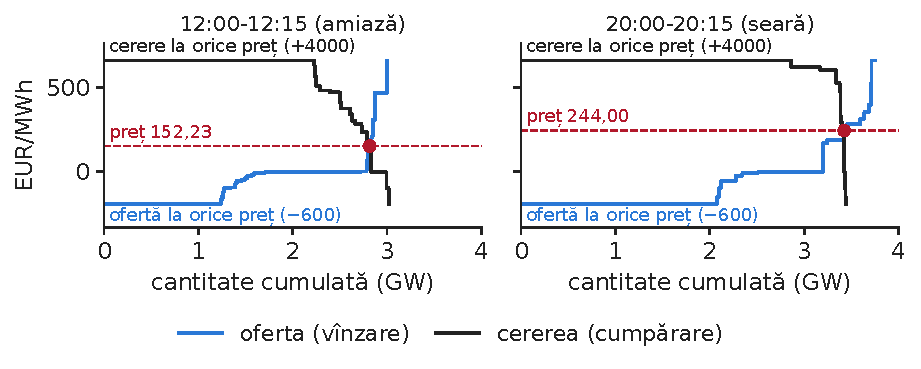
\includegraphics[width=\textwidth,height=0.515\textheight,keepaspectratio]{charts/ro/merit_opcom.pdf}\end{center}\vspace{-3mm}
\chartsource{Sursa: OPCOM, curbele agregate PZU. Date: 2026-10-21, ora României; cantitățile includ blocurile, ordinele orare și fluxurile nete.}
\vspace{0.5mm}
\begin{itemize}\setlength{\itemsep}{0pt}
  \item Aceeași zi, două prețuri: oferta se schimbă cu soarele
    \begin{itemize}\setlength{\itemsep}{0pt}
      \item La amiază: 2\,333 MW oferiți la preț zero sau negativ, preț 152{,}23 EUR/MWh
      \item Seara: fără soare, 1\,054 MW import net în ofertă, preț 244{,}00 EUR/MWh
    \end{itemize}
\end{itemize}
\par\vfill\manager{un consumator care își mută consumul de seara la amiază plătește prețul de închidere mai mic.}\par\vspace{0.5mm}
\par\vfill\noindent{\scriptsize\color{FooterGray}(OPCOM, curbele agregate PZU)}\hfill\qlink{EMQA\_L1\_merit\_opcom}{Quantlets/L1/EMQA_L1_merit_opcom}\par\vspace{0.5mm}
\end{frame}

\begin{frame}{Etapele tranzacționării pentru o zi de livrare}
\footnotesize

\begin{center}
\begin{tikzpicture}[x=1cm,y=1cm,
  box/.style={draw=MainBlue,fill=BlockGray,rounded corners=2pt,align=center,text width=3.05cm,minimum height=1.3cm,font=\scriptsize}]
\draw[-{Latex},thick,MainBlue] (0,0) -- (14.5,0);
\node[box] at (1.7,1.05) {\textbf{1. Contracte la termen}\\ piețele centralizate OPCOM și contracte bilaterale negociate direct (OTC), cu săptămîni sau ani înainte};
\node[box] at (5.3,1.05) {\textbf{2. Oferta pe PZU}\\ termen-limită: 12:00, ora Europei Centrale (CET), în ziua $d-1$ (13:00 la București); rezultatele apar la începutul după-amiezii};
\node[box] at (8.9,1.05) {\textbf{3. Ajustări intrazilnice}\\ licitații intrazilnice (IDA) și tranzacționare continuă pînă aproape de livrare};
\node[box] at (12.5,1.05) {\textbf{4. Echilibrare}\\ Transelectrica, operatorul de transport și de sistem (TSO), echilibrează sistemul; dezechilibrele se decontează la 15 min};
\foreach \x/\l in {1.7/{săptămîni--ani}, 5.3/{ziua $d-1$}, 8.9/{$d-1$ și $d$}, 12.5/{ziua $d$, în timp real}}
  \node[font=\scriptsize,below] at (\x,-0.05) {\l};
\end{tikzpicture}
\end{center}
\vspace{1mm}
\begin{itemize}\setlength{\itemsep}{1pt}
  \item \textbf{Ora și moneda}: România folosește ora Europei de Est (EET), cu o oră înaintea CET
    \begin{itemize}\setlength{\itemsep}{0pt}
      \item În cuplarea unică a piețelor pentru ziua următoare (SDAC), prețurile se exprimă în EUR, iar OPCOM le publică și în lei (RON).
    \end{itemize}
  \item \textbf{De ce contează ordinea}: fiecare etapă o corectează pe cea anterioară
    \begin{itemize}\setlength{\itemsep}{0pt}
      \item Ce nu s-a contractat la termen se cumpără pe PZU, iar ce rămîne neacoperit după piața intrazilnică se decontează ca dezechilibru.
    \end{itemize}
\end{itemize}
\par\vfill\manager{traderul își acoperă riscul la termen, licitează pe PZU pînă la ora 13:00 (ora Bucureștiului), corectează erorile pe piața intrazilnică și decontează dezechilibrul rămas.}\par\vspace{0.5mm}
\par\vfill\noindent{\scriptsize\color{FooterGray}(Maciejowska, Uniejewski \& Weron, 2023, Oxford Res.\ Enc.; OPCOM; Transelectrica)}\par\vspace{0.5mm}
\end{frame}

\begin{frame}{Cine stabilește regulile: operatori, reglementatori, limite de preț, transparență}
\footnotesize
\begin{itemize}\setlength{\itemsep}{1pt}
  \item \textbf{Cine ce face}
    \begin{itemize}\setlength{\itemsep}{0pt}
      \item OPCOM: operatorul desemnat al pieței de energie electrică (NEMO); administrează PZU și piața intrazilnică
      \item Transelectrica (TSO): conduce sistemul în timp real și decontează dezechilibrele
      \item Autoritatea Națională de Reglementare în Domeniul Energiei (ANRE): stabilește regulile și licențiază participanții
    \end{itemize}
  \item \textbf{Transparență}
    \begin{itemize}\setlength{\itemsep}{0pt}
      \item Regulamentul Uniunii Europene (UE) privind integritatea și transparența pieței angro de energie (REMIT): informațiile privilegiate se publică fără întîrziere
      \item De exemplu, opririle neplanificate ale centralelor mari; asemenea informații influențează prețul PZU
      \item Agenția UE pentru Cooperarea Autorităților de Reglementare din Domeniul Energiei (ACER) supraveghează piața pentru a depista abuzurile
    \end{itemize}
  \item \textbf{Limite de preț}
    \begin{itemize}\setlength{\itemsep}{0pt}
      \item Prețul minim armonizat în SDAC: $-500$ EUR/MWh; $-600$ pentru livrările începînd cu 29 mai 2026 (OPCOM)
      \item O serie care atinge pragul este cenzurată: prețul de echilibru ar fi fost și mai mic
    \end{itemize}
\end{itemize}
\par\vfill\manager{citiți mesajele REMIT înainte de a licita
    \begin{itemize}\setlength{\itemsep}{0pt}
      \item O oprire neplanificată anunțată la timp schimbă prețul PZU.
    \end{itemize}}\par\vspace{0.5mm}
\par\vfill\noindent{\scriptsize\color{FooterGray}(OPCOM; ANRE; ACER; Regulamentul (UE) 1227/2011)}\par\vspace{0.5mm}
\end{frame}

\subsection{Cuplarea piețelor și intervalul de 15 minute}

\begin{frame}{Cuplarea piețelor: exporturi spre zonele cu prețuri mari, pînă la limita rețelei}
\footnotesize
\intuition{Europa organizează o singură licitație comună pentru ziua următoare; zonele cu prețuri mici exportă către cele cu prețuri mari pînă la atingerea unei limite de rețea și abia atunci prețurile se separă.}
\begin{columns}[T,onlytextwidth]
\begin{column}{0.45\textwidth}
\[ \max\sum_{z}\Big[\underbrace{\textstyle\int_0^{d_z}\!D_z^{-1}}_{\text{valoare}}-\underbrace{\textstyle\int_0^{s_z}\!S_z^{-1}}_{\text{cost}}\Big]\ \text{a.î. }\underbrace{\mathbf{flows}\in\mathcal F}_{\text{limitele rețelei}} \]{\footnotesize\begin{itemize}\setlength{\itemsep}{0pt}
  \item \textbf{\txtwhere}
    \begin{itemize}\setlength{\itemsep}{0pt}
      \item $z$ = zona de ofertare
      \item $d_z, s_z$ = energia cumpărată, respectiv vîndută în $z$
      \item $\mathcal F$ = schimburile fezabile
      \item Dacă nicio limită nu este atinsă, $p_z=p_{z'}$, altfel prețurile se separă.
    \end{itemize}
\end{itemize}\par}
\end{column}
\begin{column}{0.52\textwidth}
\begin{itemize}\setlength{\itemsep}{1pt}
  \item \emph{Imagine simplificată}: o capacitate pe fiecare graniță
    \begin{itemize}\setlength{\itemsep}{0pt}
      \item Din 8 iunie 2022, la granița România--Ungaria se aplică alocarea \emph{bazată pe fluxuri} din regiunea Core
      \item La granița România--Bulgaria se păstrează alocarea capacității pe graniță.
    \end{itemize}
  \item Prețurile egale nu dovedesc absența congestiilor pe interconexiune
    \begin{itemize}\setlength{\itemsep}{0pt}
      \item O diferență de preț nu arată ce linie și-a atins limita.
    \end{itemize}
  \item Schimburile programate diferă de fluxurile fizice
    \begin{itemize}\setlength{\itemsep}{0pt}
      \item Drepturile pe termen lung se alocă prin Joint Allocation Office (JAO).
    \end{itemize}
\end{itemize}
\end{column}
\end{columns}
\par\vfill\manager{pe RO--HU, un trader cîștigă din diferența de preț doar cînd interconexiunea este saturată.}\par\vspace{0.5mm}
\par\vfill\noindent{\scriptsize\color{FooterGray}(Weron, 2014, IJF; JAO; cuplarea bazată pe fluxuri Core)}\par\vspace{0.5mm}
\end{frame}

\begin{frame}{Zece ani de cuplare: de la patru țări la o licitație europeană}
\small
\vspace{0.5mm}\begin{center}\begin{tikzpicture}[x=1cm,y=1cm]
\draw[-{Latex},thick,MainBlue] (0,0) -- (14.1,0);
\fill[MainBlue] (1.10,0) circle (2.2pt);\draw[MainBlue] (1.10,0) -- (1.10,0.63);
\node[align=center,text width=2.25cm,font=\scriptsize] at (1.10,1.15) {\textbf{2014}\\ România se cuplează cu Cehia, Slovacia și Ungaria (4M Market Coupling)};
\fill[MainBlue] (3.10,0) circle (2.2pt);\draw[MainBlue] (3.10,0) -- (3.10,-0.63);
\node[align=center,text width=2.25cm,font=\scriptsize] at (3.10,-1.15) {\textbf{19 nov. 2019}\\ aderarea la cuplarea unică a piețelor intrazilnice (SIDC)};
\fill[MainBlue] (5.10,0) circle (2.2pt);\draw[MainBlue] (5.10,0) -- (5.10,0.63);
\node[align=center,text width=2.25cm,font=\scriptsize] at (5.10,1.15) {\textbf{17 iun. 2021}\\ aderarea la SDAC, prin cuplarea interimară 4M};
\fill[MainBlue] (7.10,0) circle (2.2pt);\draw[MainBlue] (7.10,0) -- (7.10,-0.63);
\node[align=center,text width=2.25cm,font=\scriptsize] at (7.10,-1.15) {\textbf{27 oct. 2021}\\ cuplarea graniței Bulgaria--România în SDAC};
\fill[MainBlue] (9.10,0) circle (2.2pt);\draw[MainBlue] (9.10,0) -- (9.10,0.63);
\node[align=center,text width=2.25cm,font=\scriptsize] at (9.10,1.15) {\textbf{8 iun. 2022}\\ alocarea bazată pe fluxuri în regiunea Core (România--Ungaria)};
\fill[MainBlue] (11.10,0) circle (2.2pt);\draw[MainBlue] (11.10,0) -- (11.10,-0.63);
\node[align=center,text width=2.25cm,font=\scriptsize] at (11.10,-1.15) {\textbf{mar. 2025}\\ granițele României intră în licitațiile intrazilnice};
\fill[MainBlue] (13.10,0) circle (2.2pt);\draw[MainBlue] (13.10,0) -- (13.10,0.63);
\node[align=center,text width=2.25cm,font=\scriptsize] at (13.10,1.15) {\textbf{1 oct. 2025}\\ intervalul de 15 minute în SDAC};
\end{tikzpicture}\end{center}
\vspace{0.5mm}
\begin{itemize}\setlength{\itemsep}{1pt}
  \item Prețurile se calculează cu algoritmul hibrid paneuropean de integrare a piețelor de energie electrică (EUPHEMIA).
  \item Fiecare etapă a schimbat datele: vecini noi, produse noi, o rezoluție mai fină
    \begin{itemize}\setlength{\itemsep}{0pt}
      \item Verificați data înainte de a compara perioade.
    \end{itemize}
\end{itemize}
\par\vfill\noindent{\scriptsize\color{FooterGray}(comunicate OPCOM 2019--2025; IBEX/OPCOM, 27 oct. 2021; JAO)}\par\vspace{0.5mm}
\end{frame}

\begin{frame}{Din 1 octombrie 2025, o zi are 96 de prețuri, nu 24}
\footnotesize
\intuition{Intervalul de tranzacționare (MTU) s-a redus de la o oră la 15 minute, așa că numărul intervalelor trebuie convertit în ore echivalente.}
\begin{columns}[T,onlytextwidth]
\begin{column}{0.53\textwidth}
\[ \bar p_d=\frac{1}{M_d}\sum_{m=1}^{M_d}p_{d,m},\qquad H_y=\sum_{t\in y}\underbrace{\mathbb 1\{p_t<0\}}_{\text{1 dacă } p_t<0}\cdot\underbrace{\Delta_t/60}_{\text{durata în ore}} \]{\footnotesize\begin{itemize}\setlength{\itemsep}{0pt}
  \item \textbf{\txtwhere}
    \begin{itemize}\setlength{\itemsep}{0pt}
      \item $p_{d,m}$ = prețul intervalului $m$ din ziua $d$
      \item $M_d$ = numărul de intervale din zi: 96 din oct. 2025, 24 înainte ($\pm$1 oră la schimbarea orei de vară (DST))
      \item $\bar p_d$ = \emph{prețul mediu zilnic al energiei în bandă}
      \item $\Delta_t\in\{60,15\}$ = durata intervalului, în minute
      \item $H_y$ = numărul de ore echivalente din anul $y$.
    \end{itemize}
\end{itemize}\par}
\end{column}
\begin{column}{0.44\textwidth}
\begin{itemize}\setlength{\itemsep}{1pt}
  \item \textbf{Conform datelor}
    \begin{itemize}\setlength{\itemsep}{0pt}
      \item 94\,222 de intervale orare pînă în sep. 2025 și 38\,020 de sferturi de oră de atunci
      \item Ian.--oct. 2026: 687 de sferturi de oră cu preț negativ în România, adică 171{,}75 h
      \item Numărate ca ore, durata ar fi supraevaluată de 4 ori
    \end{itemize}
\end{itemize}
\end{column}
\end{columns}
\par\vfill\manager{întrebați mereu „ore sau sferturi de oră?” înainte de a compara anii între ei.}\par\vspace{0.5mm}
\par\vfill\noindent{\scriptsize\color{FooterGray}(OPCOM, 1 oct. 2025)}\hfill\tryit{notebook-ul Jupyter \S1}\par\vspace{0.5mm}
\end{frame}

\subsection{Ce produce România}

\begin{frame}{Producția României: hidro, nuclear, gaze, cărbune și tot mai mult solar}
\small
\begin{center}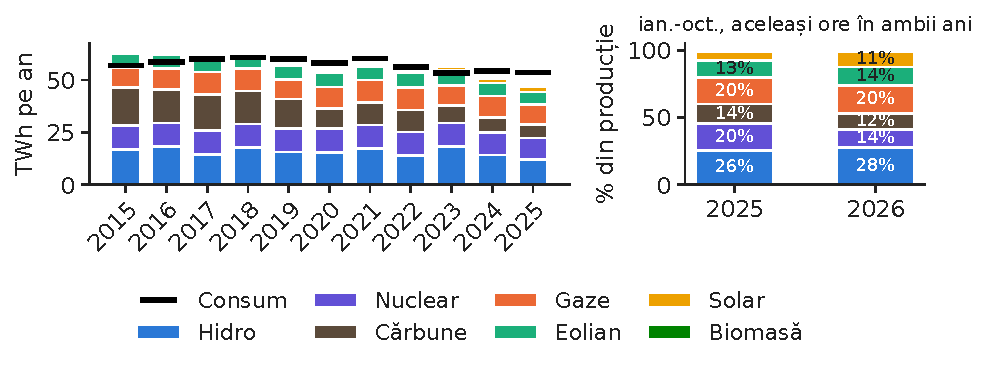
\includegraphics[width=\textwidth,height=0.525\textheight,keepaspectratio]{charts/ro/mix_ro_annual.pdf}\end{center}\vspace{-3mm}
\chartsource{Sursa: energy-charts.info (Fraunhofer ISE); ENTSO-E (date Transelectrica pentru România). Date: 2015-2025 ani compleți (stînga); ian.-oct. 2025 și 2026, ore raportate în ambii ani (dreapta); date pînă la 2026-10-31.}
\vspace{0.5mm}
\begin{itemize}\setlength{\itemsep}{0pt}
  \item Hidro = centrale pe firul apei (RoR) + centrale cu lac de acumulare, cărbune = lignit + huilă
    \begin{itemize}\setlength{\itemsep}{0pt}
      \item Bara neagră reprezintă consumul, iar deasupra coloanei de producție indică import net
      \item Energia este însumată pe orele raportate (acoperire $\ge$ 98{,}1\% în anii compleți)
      \item Datele solare măsurate pot exclude producția panourilor de pe acoperișuri.
    \end{itemize}
\end{itemize}
\par\vfill\noindent{\scriptsize\color{FooterGray}(energy-charts.info; sursa datelor: ENTSO-E)}\hfill\qlink{EMQA\_L1\_mix\_ro\_annual}{Quantlets/L1/EMQA_L1_mix_ro_annual}\par\vspace{0.5mm}
\end{frame}

\begin{frame}{România: cărbunele scade, solarul crește, iar nuclearul se reduce în 2026}
\small
\begin{center}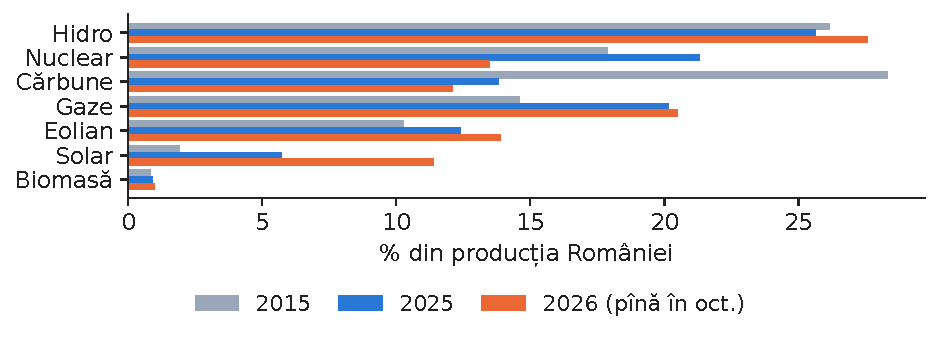
\includegraphics[width=\textwidth,height=0.436\textheight,keepaspectratio]{charts/ro/mix_shares.pdf}\end{center}\vspace{-3mm}
\chartsource{Sursa: energy-charts.info (Fraunhofer ISE); ENTSO-E (date Transelectrica pentru România). Date: 2015, 2025 ani compleți; ian.-oct. 2026, ore raportate și în 2025, și în 2026.}
\vspace{0.5mm}
\begin{itemize}\setlength{\itemsep}{0pt}
  \item Producția pe cărbune: \ensuremath{-}63{,}9\% între 2015 și 2025
    \begin{itemize}\setlength{\itemsep}{0pt}
      \item În aceeași perioadă, solarul măsurat a crescut de 2{,}2 ori.
    \end{itemize}
  \item Nuclear, ian.--oct. 2026 față de 2025: \ensuremath{-}31{,}3\% pe orele raportate în ambii ani
    \begin{itemize}\setlength{\itemsep}{0pt}
      \item Limită inferioară: cele 29 de zile neraportate din septembrie sînt excluse.
    \end{itemize}
\end{itemize}
\par\vfill\manager{cînd lipsește apa sau un reactor, prețul este stabilit de o altă centrală.}\par\vspace{0.5mm}
\par\vfill\noindent{\scriptsize\color{FooterGray}(România; energy-charts.info; sursa datelor: ENTSO-E)}\hfill\qlink{EMQA\_L1\_mix\_shares}{Quantlets/L1/EMQA_L1_mix_shares}\par\vspace{0.5mm}
\end{frame}

\begin{frame}{Structura cursului: șapte prelegeri și o hartă a modelelor}
\footnotesize
\begin{columns}[T,onlytextwidth]
\begin{column}{0.56\textwidth}
\begin{block}{Planul cursului}
\begin{enumerate}\setlength{\itemsep}{0pt}\footnotesize
\item \textbf{Piețele de energie și datele lor} (astăzi)
\item Prognoza: modele clasice și modele autoregresive cu variabile exogene (ARX)
\item Volatilitatea
\item Riscul în companiile de energie: preț--volum, flux de numerar la risc, dezechilibre, risc de bază
\item Derivate și acoperirea riscului, inclusiv contractele de achiziție de energie (PPA)
\item Regenerabile, stocare, flexibilitate: canibalizare, prețuri negative, baterii
\item Învățare automată și modele fundaționale pentru prognoză
\end{enumerate}
\end{block}
\end{column}
\begin{column}{0.41\textwidth}
\begin{itemize}\setlength{\itemsep}{1pt}
  \item \textbf{Familii de modele}
    \begin{itemize}\setlength{\itemsep}{0pt}
      \item Fundamentale: curba ofertei, costul combustibilului și al CO$_2$
      \item De formă redusă (revenire la medie, salturi) și statistice
      \item Învățare automată și modele hibride
    \end{itemize}
  \item \textbf{Două perspective asupra acelorași date}
    \begin{itemize}\setlength{\itemsep}{0pt}
      \item Univariată: o singură serie lungă de prețuri
      \item Multivariată: 24 (acum 96) de serii zilnice, cîte una pe interval
    \end{itemize}
  \item Orice model trebuie să depășească \textbf{prognoza naivă} din secțiunea 3.
\end{itemize}
\end{column}
\end{columns}
\par\vfill\manager{întrebați furnizorul de prognoze din ce familie face parte modelul și cu cît depășește prognoza naivă.}\par\vspace{0.5mm}
\par\vfill\noindent{\scriptsize\color{FooterGray}(Weron, 2014, IJF; Ziel \& Weron, 2018, ENEECO)}\par\vspace{0.5mm}
\end{frame}


\section{Date din energie și fapte stilizate}

\subsection{Unități de măsură, fusuri orare și date curate}

\begin{frame}{Putere și energie: MW nu înseamnă MWh}
\footnotesize
\intuition{Un megawatt (MW) măsoară puterea, adică ritmul producției sau al consumului; un megawatt-oră (MWh) măsoară cantitatea de energie, de exemplu 1 MW timp de o oră.}
\begin{columns}[T,onlytextwidth]
\begin{column}{0.45\textwidth}
\[ E=\frac{1}{10^6}\sum_{t\ \text{raportat}}\underbrace{P_t\,\Delta_t}_{\text{MWh}}\ [\text{TWh}] \]\[ \text{acoperire}=\frac{\text{ore raportate}}{\text{ore din perioadă}} \]{\footnotesize\begin{itemize}\setlength{\itemsep}{0pt}
  \item \textbf{\txtwhere}
    \begin{itemize}\setlength{\itemsep}{0pt}
      \item $P_t$ = puterea medie în intervalul $t$ (MW)
      \item $\Delta_t$ = durata intervalului (h)
      \item $E$ = energia, în terawați-oră (TWh), $1\ \text{TWh}=10^6\ \text{MWh}$.
    \end{itemize}
\end{itemize}\par}
\end{column}
\begin{column}{0.52\textwidth}
\begin{itemize}\setlength{\itemsep}{0pt}
  \item \textbf{Conform datelor}: România a consumat 53{,}56 TWh în 2025, adică o putere medie de 6{,}1 gigawați (GW).
  \item Orele lipsă nu se completează, iar fiecare total are alături gradul de acoperire.
  \item \textbf{Prețuri de referință}
    \begin{itemize}\setlength{\itemsep}{0pt}
      \item În bandă (base): media prețurilor zilei de livrare
      \item De vîrf (peak): prețul mediu 08:00--20:00, luni--vineri
    \end{itemize}
  \item Gazele și țițeiul se cotează în dolari americani (USD) pe milion de unități termice britanice (MMBtu), respectiv pe baril (bbl)
    \begin{itemize}\setlength{\itemsep}{0pt}
      \item Conversia în EUR/MWh: Anexa G.
    \end{itemize}
\end{itemize}
\end{column}
\end{columns}
\par\vfill\manager{un contract de 10 MW în bandă înseamnă 240 MWh livrați pe zi.}\par\vspace{0.5mm}
\par\vfill\noindent{\scriptsize\color{FooterGray}(energy-charts.info; Banca Mondială)}\hfill\tryit{notebook-ul Jupyter \S1}\par\vspace{0.5mm}
\end{frame}

\begin{frame}{O zi de consum în România: puterea în MW, energia în MWh}
\small
\begin{center}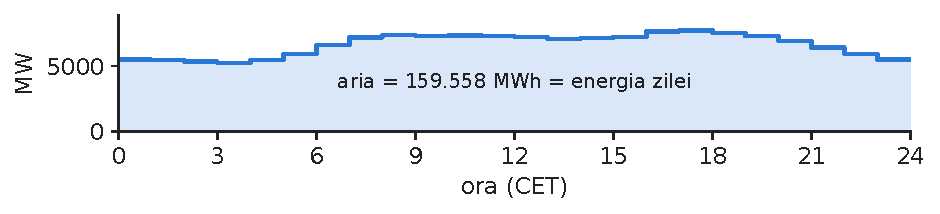
\includegraphics[width=\textwidth,height=0.427\textheight,keepaspectratio]{charts/ro/day_load.pdf}\end{center}\vspace{-3mm}
\chartsource{Sursa: energy-charts.info (Fraunhofer ISE); ENTSO-E (date Transelectrica pentru România). Date: România, consumul din 2026-10-28 (zi CET, 24 de valori orare).}
\vspace{0.5mm}
\begin{itemize}\setlength{\itemsep}{0pt}
  \item \textbf{Curba} arată puterea: cît consumă țara în fiecare oră (MW)
    \begin{itemize}\setlength{\itemsep}{0pt}
      \item Minimum 5\,253 MW la ora 3:00, maximum 7\,719 MW la ora 17:00 (CET)
    \end{itemize}
  \item \textbf{Aria colorată} este energia: 159\,558 MWh pe 28 octombrie 2026
    \begin{itemize}\setlength{\itemsep}{0pt}
      \item 24 de ore $\times$ o putere medie de 6\,648 MW
    \end{itemize}
\end{itemize}
\par\vfill\manager{un furnizor cumpără energie (MWh), iar rețeaua trebuie să acopere puterea de vîrf (MW).}\par\vspace{0.5mm}
\par\vfill\noindent{\scriptsize\color{FooterGray}(România; energy-charts.info; sursa datelor: ENTSO-E)}\hfill\qlink{EMQA\_L1\_day\_load}{Quantlets/L1/EMQA_L1_day_load}\par\vspace{0.5mm}
\end{frame}

\begin{frame}{Pregătirea datelor (1): ziua de livrare, schimbarea orei și a zonei}
\footnotesize
\begin{itemize}\setlength{\itemsep}{1pt}
  \item \textbf{Fusuri orare}: marcajele temporale din datele brute sînt în timpul universal coordonat (UTC)
    \begin{itemize}\setlength{\itemsep}{0pt}
      \item Statisticile zilnice folosesc ziua de livrare din SDAC, în ora Europei Centrale (CET) sau, vara, în ora de vară a Europei Centrale (CEST)
      \item O zi UTC ar muta una sau două ore în ziua greșită.
    \end{itemize}
  \item \textbf{Schimbarea orei}: ultima duminică din martie are 23 de ore, ultima duminică din octombrie are 25
    \begin{itemize}\setlength{\itemsep}{0pt}
      \item Mediile zilnice folosesc intervalele care există efectiv.
    \end{itemize}
  \item \textbf{Schimbarea zonei}: Germania--Austria--Luxemburg a fost o singură zonă de ofertare pînă la 30 sep. 2018
    \begin{itemize}\setlength{\itemsep}{0pt}
      \item Seria noastră le îmbină la acea dată.
    \end{itemize}
  \item Fiecare grafic și fiecare cifră pot fi reproduse în notebook-ul Jupyter al cursului
    \begin{itemize}\setlength{\itemsep}{0pt}
      \item Un singur grafic, marcat ca atare, folosește date simulate (zgomot alb, mers aleator).
    \end{itemize}
\end{itemize}
\par\vfill\noindent{\scriptsize\color{FooterGray}(Lago, Marcjasz, De Schutter \& Weron, 2021, APEN)}\hfill\tryit{notebook-ul Jupyter \S1}\par\vspace{0.5mm}
\end{frame}

\begin{frame}{Pregătirea datelor (2): zile lipsă și rupturi de serie}
\footnotesize
\begin{itemize}\setlength{\itemsep}{1pt}
  \item \textbf{Zile lipsă}: sursa (energy-charts.info, care republică prețurile OPCOM și ale bursei independente de energie din Bulgaria (IBEX) raportate la ENTSO-E) nu are preț pentru unele zile și nu indică motivul
    \begin{itemize}\setlength{\itemsep}{0pt}
      \item România: 5 zile (21 septembrie 2015, 20 decembrie 2015, 21 decembrie 2015, 31 decembrie 2017, 17 august 2018)
      \item Bulgaria: seria începe la 31 octombrie 2016, deși bursa IBEX organizează piața pentru ziua următoare din 19 ianuarie 2016, și mai lipsesc 15 zile pînă la 31 decembrie 2016
      \item Aceste zile nu se completează, iar variația zilnică nu se calculează peste un gol.
    \end{itemize}
  \item \textbf{Schimbarea contractului futures}: seria Brent poate prezenta un salt la trecerea la contractul următor
    \begin{itemize}\setlength{\itemsep}{0pt}
      \item Aceste zile sînt excluse din statisticile randamentelor.
    \end{itemize}
\end{itemize}
\par\vfill\manager{la un furnizor, cele mai multe erori de prognoză apar la prelucrarea datelor (fus orar greșit, goluri completate), nu în model.}\par\vspace{0.5mm}
\par\vfill\noindent{\scriptsize\color{FooterGray}(Lago, Marcjasz, De Schutter \& Weron, 2021, APEN)}\hfill\tryit{notebook-ul Jupyter \S1}\par\vspace{0.5mm}
\end{frame}

\subsection{Nivelul prețurilor și sezonalitatea}

\begin{frame}{Prețurile au explodat în 2021--2022 și nu au mai revenit la vechiul nivel}
\small
\begin{center}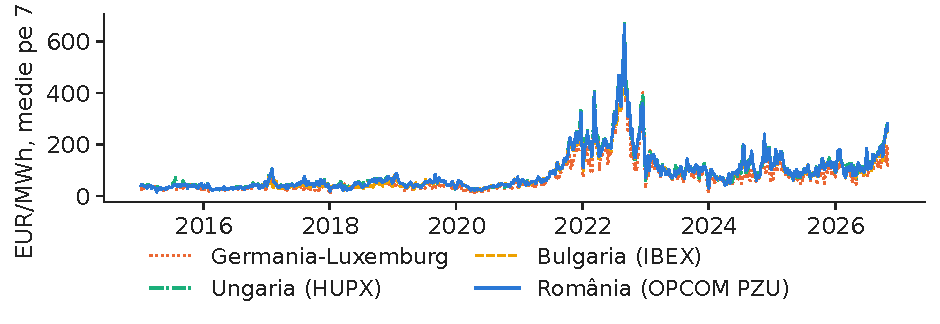
\includegraphics[width=\textwidth,height=0.486\textheight,keepaspectratio]{charts/ro/prices_daily_4zones.pdf}\end{center}\vspace{-3mm}
\chartsource{Sursa: energy-charts.info (Fraunhofer ISE); prețurile burselor OPCOM, IBEX, HUPX, EPEX SPOT, prin ENTSO-E. Date: 2015-01-01 - 2026-10-31 (BG din 2016-10-31).}
\vspace{0.5mm}
\begin{itemize}\setlength{\itemsep}{0pt}
  \item Maximul zilnic din România: 738{,}28 EUR/MWh, la 30 august 2022
    \begin{itemize}\setlength{\itemsep}{0pt}
      \item RO, BG și HU evoluează împreună (piețe cuplate), iar Germania este mai ieftină din 2023.
    \end{itemize}
\end{itemize}
\par\vfill\manager{un consumator industrial care își face bugetul cu prețurile de dinainte de 2021 le subestimează de două-trei ori.}\par\vspace{0.5mm}
\par\vfill\noindent{\scriptsize\color{FooterGray}(energy-charts.info; prețuri: OPCOM, IBEX, HUPX, EPEX SPOT)}\hfill\qlink{EMQA\_L1\_prices\_daily\_4zones}{Quantlets/L1/EMQA_L1_prices_daily_4zones}\par\vspace{0.5mm}
\end{frame}

\begin{frame}{Volatilitatea crește odată cu nivelul prețului}
\small
{\footnotesize\renewcommand{\arraystretch}{1.05}\setlength{\tabcolsep}{4pt}
\begin{tabular}{@{}lrrrrrrrrr@{}}\toprule
Media, EUR/MWh & 2018 & 2019 & 2020 & 2021 & 2022 & 2023 & 2024 & 2025 & 2026 YTD \\ \midrule
RO & \cellcolor{Forest!52}46{,}4 & \cellcolor{Forest!50}50{,}4 & \cellcolor{Forest!55}39{,}5 & \cellcolor{Forest!20}111{,}4 & \cellcolor{Crimson!55}265{,}3 & \cellcolor{Forest!24}103{,}7 & \cellcolor{Forest!24}103{,}5 & \cellcolor{Forest!22}108{,}2 & \cellcolor{Forest!7}137{,}4 \\
BG & \cellcolor{Forest!55}39{,}9 & \cellcolor{Forest!51}47{,}5 & \cellcolor{Forest!55}39{,}3 & \cellcolor{Forest!19}108{,}7 & \cellcolor{Crimson!55}252{,}8 & \cellcolor{Forest!22}103{,}8 & \cellcolor{Forest!22}102{,}5 & \cellcolor{Forest!20}106{,}9 & \cellcolor{Forest!8}129{,}9 \\
HU & \cellcolor{Forest!49}51{,}0 & \cellcolor{Forest!50}50{,}4 & \cellcolor{Forest!55}39{,}0 & \cellcolor{Forest!20}113{,}8 & \cellcolor{Crimson!55}271{,}7 & \cellcolor{Forest!23}106{,}8 & \cellcolor{Forest!26}100{,}8 & \cellcolor{Forest!22}108{,}5 & \cellcolor{Forest!7}141{,}0 \\
DE-LU & \cellcolor{Forest!47}44{,}5 & \cellcolor{Forest!51}37{,}7 & \cellcolor{Forest!55}30{,}5 & \cellcolor{Forest!19}96{,}8 & \cellcolor{Crimson!55}235{,}5 & \cellcolor{Forest!20}95{,}2 & \cellcolor{Forest!29}78{,}5 & \cellcolor{Forest!23}89{,}3 & \cellcolor{Forest!10}114{,}0 \\
\multicolumn{10}{@{}l}{\textit{Volatilitate: abaterea standard a variațiilor zilnice ale prețului}} \\
RO & \cellcolor{Forest!50}10{,}9 & \cellcolor{Forest!49}11{,}5 & \cellcolor{Forest!55}8{,}6 & \cellcolor{Forest!19}25{,}2 & \cellcolor{Crimson!55}58{,}9 & \cellcolor{Forest!16}26{,}3 & \cellcolor{Forest!3}32{,}4 & \cellcolor{Forest!20}24{,}4 & \cellcolor{Forest!5}31{,}6 \\
BG & \cellcolor{Forest!46}13{,}6 & \cellcolor{Forest!48}12{,}8 & \cellcolor{Forest!55}9{,}8 & \cellcolor{Forest!23}23{,}6 & \cellcolor{Crimson!55}56{,}6 & \cellcolor{Forest!16}26{,}2 & \cellcolor{Forest!4}31{,}5 & \cellcolor{Forest!22}23{,}9 & \cellcolor{Forest!12}28{,}2 \\
HU & \cellcolor{Forest!53}9{,}2 & \cellcolor{Forest!53}9{,}2 & \cellcolor{Forest!55}8{,}5 & \cellcolor{Forest!18}24{,}8 & \cellcolor{Crimson!55}56{,}6 & \cellcolor{Forest!17}25{,}0 & \cellcolor{Crimson!5}34{,}7 & \cellcolor{Forest!17}25{,}3 & 32{,}6 \\
DE-LU & \cellcolor{Forest!55}11{,}5 & \cellcolor{Forest!54}11{,}9 & \cellcolor{Forest!55}11{,}5 & \cellcolor{Forest!8}34{,}4 & \cellcolor{Crimson!55}65{,}3 & \cellcolor{Forest!17}30{,}3 & \cellcolor{Forest!14}31{,}4 & \cellcolor{Forest!21}28{,}3 & \cellcolor{Forest!5}36{,}0 \\
\bottomrule\end{tabular}}
\par\vspace{0.5mm}{\scriptsize \begin{itemize}\setlength{\itemsep}{0pt}
  \item Culoarea, pe fiecare rînd: verde = valoarea minimă, roșu = valoarea maximă (2026 YTD = ian.--oct. 2026).
\end{itemize}}
\vspace{1mm}
\begin{itemize}\setlength{\itemsep}{1pt}
  \item 2026 YTD: România 137{,}45 EUR/MWh, față de 105{,}88 EUR/MWh în ian.--oct. 2025 (\ensuremath{+}29{,}8\%).
\end{itemize}
\par\vfill\manager{garanțiile pentru PZU cresc odată cu prețul: la 200 EUR/MWh piața fluctuează mult mai mult decît la 50.}\par\vspace{0.5mm}
\par\vfill\noindent{\scriptsize\color{FooterGray}(energy-charts.info; calcule proprii)}\par\vspace{0.5mm}
\end{frame}

\begin{frame}{Producția solară a mutat minimul zilnic al prețului la amiază}
\small
\begin{center}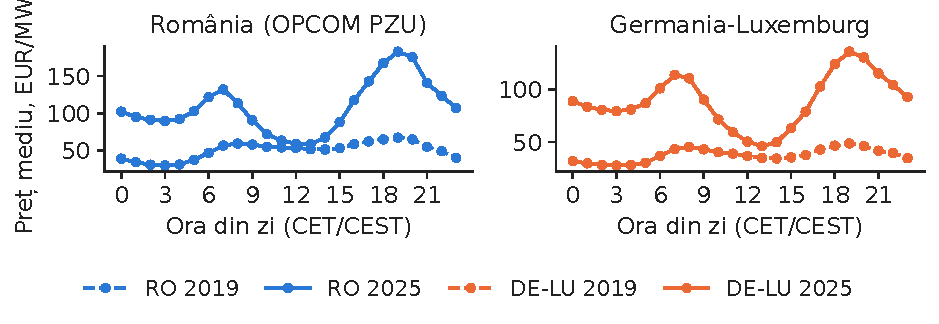
\includegraphics[width=\textwidth,height=0.438\textheight,keepaspectratio]{charts/ro/profile_intraday.pdf}\end{center}\vspace{-3mm}
\chartsource{Sursa: energy-charts.info (Fraunhofer ISE); prețurile burselor OPCOM, IBEX, HUPX, EPEX SPOT, prin ENTSO-E. Date: anii 2019 și 2025, date orare.}
\vspace{0.5mm}
\begin{itemize}\setlength{\itemsep}{0pt}
  \item Între 2019 și 2025, ora cu prețul minim s-a deplasat din timpul nopții către amiază
    \begin{itemize}\setlength{\itemsep}{0pt}
      \item 2025: minimul la ora 13:00 (58{,}8 EUR/MWh în România), vîrful de seară la 182{,}5
      \item Raportul seară/amiază a urcat de la 1{,}30 la 3{,}11: „curba în formă de rață” (duck curve).
    \end{itemize}
\end{itemize}
\par\vfill\manager{venitul unei baterii provine din această diferență dintre amiază și seară, valorificată o dată sau de două ori pe zi.}\par\vspace{0.5mm}
\par\vfill\noindent{\scriptsize\color{FooterGray}(energy-charts.info; prețuri orare PZU)}\hfill\qlink{EMQA\_L1\_profile\_intraday}{Quantlets/L1/EMQA_L1_profile_intraday}\par\vspace{0.5mm}
\end{frame}

\begin{frame}{La sfîrșit de săptămînă, energia este mai ieftină}
\footnotesize
\intuition{În weekend, fabricile și birourile consumă mai puțin, sînt necesare mai puține centrale și prețul scade.}
\begin{columns}[T,onlytextwidth]
\begin{column}{0.50\textwidth}
\[ \hat s_j=\frac1W\sum_{w=1}^{W}\Big(\underbrace{p_{w,j}}_{\text{ziua }j\text{ din săptămîna }w}-\underbrace{\tfrac17\textstyle\sum_{i=1}^{7}p_{w,i}}_{\text{media săptămînii }w}\Big) \]{\footnotesize\begin{itemize}\setlength{\itemsep}{0pt}
  \item \textbf{\txtwhere}
    \begin{itemize}\setlength{\itemsep}{0pt}
      \item $j$ = ziua săptămînii
      \item $W$ = numărul de săptămîni complete
      \item $\hat s_j$ = abaterea medie a zilei $j$ față de media săptămînii din care face parte (EUR/MWh)
      \item Scăderea mediei săptămînale elimină salturile de nivel, ca în 2022.
    \end{itemize}
\end{itemize}\par}
\end{column}
\begin{column}{0.47\textwidth}
\begin{itemize}\setlength{\itemsep}{1pt}
  \item \textbf{Conform datelor}: 199 de săptămîni, 2 ianuarie 2023 -- 25 octombrie 2026.
\end{itemize}\vspace{0.5mm}{\scriptsize\renewcommand{\arraystretch}{1.05}\setlength{\tabcolsep}{4pt}
\begin{tabular}{@{}lrrrrrrr@{}}\toprule
 & Lu & Ma & Mi & Jo & Vi & Sî & Du \\ \midrule
RO & \cellcolor{Crimson!46}9{,}1 & \cellcolor{Crimson!55}12{,}7 & \cellcolor{Crimson!55}12{,}6 & \cellcolor{Crimson!49}10{,}4 & \cellcolor{Crimson!31}3{,}4 & \cellcolor{Forest!22}\ensuremath{-}17{,}5 & \cellcolor{Forest!55}\ensuremath{-}30{,}7 \\
DE-LU & \cellcolor{Crimson!41}7{,}0 & \cellcolor{Crimson!53}11{,}0 & \cellcolor{Crimson!55}11{,}6 & \cellcolor{Crimson!44}7{,}9 & \cellcolor{Crimson!30}3{,}3 & \cellcolor{Forest!27}\ensuremath{-}15{,}8 & \cellcolor{Forest!55}\ensuremath{-}25{,}1 \\
\bottomrule\end{tabular}}\par\vspace{1mm}\begin{itemize}\setlength{\itemsep}{1pt}
  \item Duminica, în România: $\hat s_{\text{Du}}=$ \ensuremath{-}30{,}7 EUR/MWh față de media săptămînii.
\end{itemize}
\end{column}
\end{columns}
\par\vfill\manager{un consumator industrial își poate muta consumul flexibil (mentenanță, pompare, încărcare) duminica, reducîndu-și astfel costurile cu energia.}\par\vspace{0.5mm}
\par\vfill\noindent{\scriptsize\color{FooterGray}}\hfill\tryit{notebook-ul Jupyter \S3}\par\vspace{0.5mm}
\end{frame}

\begin{frame}{Primăvara, energia este ieftină: multă apă, mult soare, cerere moderată}
\small
\begin{center}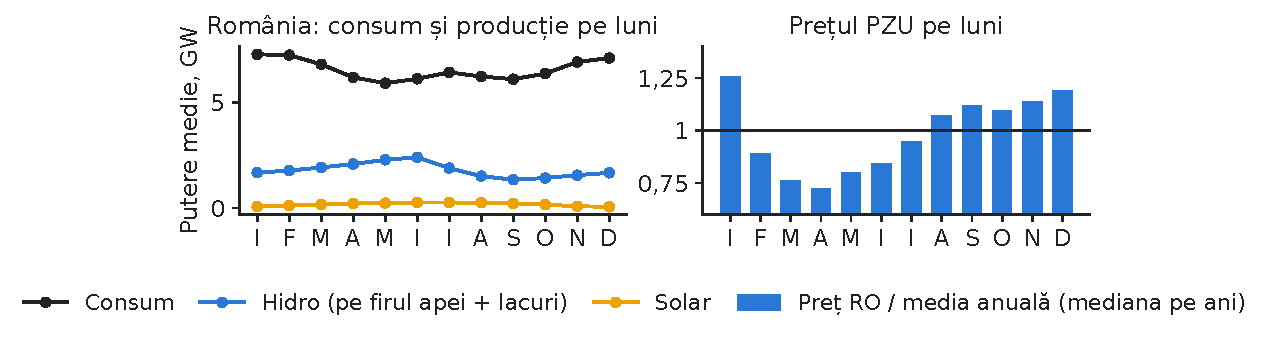
\includegraphics[width=\textwidth,height=0.437\textheight,keepaspectratio]{charts/ro/profile_annual.pdf}\end{center}\vspace{-3mm}
\chartsource{Sursa: energy-charts.info (Fraunhofer ISE); prețurile burselor OPCOM, IBEX, HUPX, EPEX SPOT, prin ENTSO-E. Date: medii lunare 2016-2025.}
\vspace{0.5mm}
\begin{itemize}\setlength{\itemsep}{0pt}
  \item Prețul raportat la media anuală: maxim în ianuarie (1{,}26), minim în aprilie (0{,}72)
    \begin{itemize}\setlength{\itemsep}{0pt}
      \item Consumul este maxim în ianuarie--februarie și minim în mai
      \item Producția hidro atinge maximul în iunie (topirea zăpezii).
    \end{itemize}
\end{itemize}
\par\vfill\manager{un producător hidro economisește apa din lacuri primăvara, cînd energia este ieftină, pentru a o turbina iarna și la sfîrșitul verii.}\par\vspace{0.5mm}
\par\vfill\noindent{\scriptsize\color{FooterGray}(energy-charts.info; medii lunare 2016--2025)}\hfill\qlink{EMQA\_L1\_profile\_annual}{Quantlets/L1/EMQA_L1_profile_annual}\par\vspace{0.5mm}
\end{frame}

\subsection{Salturi de preț și prețuri negative}

\begin{frame}{Salturile de preț: puține ore, prețuri extreme}
\footnotesize
\intuition{Un salt de preț (spike) apare într-un interval în care prețul depășește cu mult nivelul obișnuit al anului respectiv.}
\begin{columns}[T,onlytextwidth]
\begin{column}{0.55\textwidth}
\[ p_t>\underbrace{Q_{3,y}}_{\text{percentila 75}}+3\cdot\underbrace{(Q_{3,y}-Q_{1,y})}_{\text{abaterea intercuartilică (IQR)}} \]{\footnotesize\begin{itemize}\setlength{\itemsep}{0pt}
  \item \textbf{\txtwhere}
    \begin{itemize}\setlength{\itemsep}{0pt}
      \item $Q_{1,y},Q_{3,y}$ = percentilele 25 și 75 ale prețurilor din anul $y$, ponderate cu durata intervalului (un interval de 15 min are un sfert din ponderea unui interval orar)
      \item Percentilele sînt robuste, deci salturile abia mișcă pragul.
    \end{itemize}
\end{itemize}\par}
\end{column}
\begin{column}{0.42\textwidth}
{\scriptsize\renewcommand{\arraystretch}{1.0}\setlength{\tabcolsep}{4pt}
\begin{tabular}{@{}lrrr@{}}\toprule
Anul & Prag RO & RO h & DE-LU h \\ \midrule
2020 & 109 & \cellcolor{MainBlue!12}54{,}00 & \cellcolor{MainBlue!6}30{,}00 \\
2021 & 394 & \cellcolor{MainBlue!15}69{,}00 & \cellcolor{MainBlue!60}\textcolor{white}{280{,}00} \\
2022 & 873 & \cellcolor{MainBlue!1}4{,}00 & \cellcolor{MainBlue!1}4{,}00 \\
2023 & 292 & \cellcolor{MainBlue!8}38{,}00 & \cellcolor{MainBlue!3}13{,}00 \\
2024 & 274 & \cellcolor{MainBlue!59}\textcolor{white}{276{,}00} & \cellcolor{MainBlue!15}72{,}00 \\
2025 & 285 & \cellcolor{MainBlue!26}120{,}00 & \cellcolor{MainBlue!19}88{,}75 \\
2026 & 427 & \cellcolor{MainBlue!8}39{,}25 & \cellcolor{MainBlue!7}32{,}25 \\
\bottomrule\end{tabular}}\par\vspace{1mm}\begin{itemize}\setlength{\itemsep}{1pt}
  \item Cel mai mare preț din România în datele noastre: 1021{,}61 EUR/MWh, la 3 septembrie 2024, ora 19:00 CEST.
\end{itemize}
\end{column}
\end{columns}
\par\vfill\manager{un furnizor cu contracte la preț fix își poate pierde cea mai mare parte a marjei anuale în cîteva zeci de ore cu salturi de preț, motiv pentru care își acoperă riscul.}\par\vspace{0.5mm}
\par\vfill\noindent{\scriptsize\color{FooterGray}(Janczura, Trück, Weron \& Wolff, 2013, ENEECO)}\hfill\tryit{notebook-ul Jupyter \S4}\par\vspace{0.5mm}
\end{frame}

\begin{frame}{Prețurile negative au apărut în România în 2023 și au devenit frecvente}
\small
\begin{center}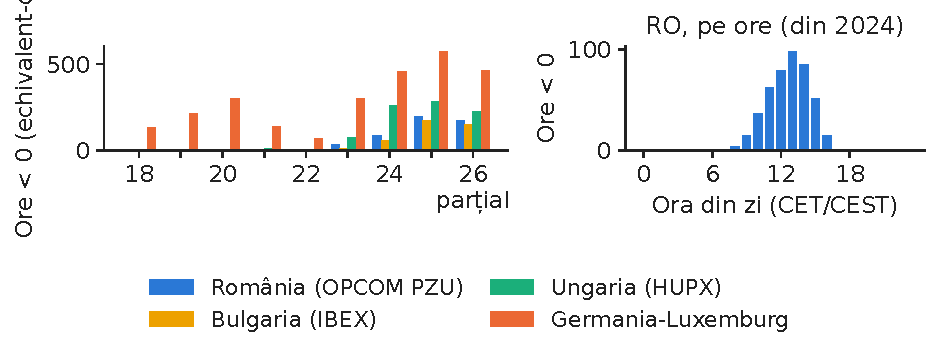
\includegraphics[width=\textwidth,height=0.442\textheight,keepaspectratio]{charts/ro/negative_prices.pdf}\end{center}\vspace{-3mm}
\chartsource{Sursa: energy-charts.info (Fraunhofer ISE); prețurile burselor OPCOM, IBEX, HUPX, EPEX SPOT, prin ENTSO-E. Date: 2018 - 2026-10-31; un interval de 15 min = 0,25 h.}
\vspace{0.5mm}
\begin{itemize}\setlength{\itemsep}{0pt}
  \item Primul preț negativ în România: 21 mai 2023
    \begin{itemize}\setlength{\itemsep}{0pt}
      \item Din 2024, 91{,}1\% din orele cu preț negativ cad între 10:00 și 16:00, iar 83{,}9\% în weekend
      \item Barele sînt în ore echivalente.
    \end{itemize}
\end{itemize}
\par\vfill\manager{un parc solar fără stocare își vinde o mare parte din producție în cele mai ieftine ore ale anului (cursul 6).}\par\vspace{0.5mm}
\par\vfill\noindent{\scriptsize\color{FooterGray}(energy-charts.info; numărare proprie, 15 min = 0,25 h)}\hfill\qlink{EMQA\_L1\_negative\_prices}{Quantlets/L1/EMQA_L1_negative_prices}\par\vspace{0.5mm}
\end{frame}

\begin{frame}{Prețurile negative, numărate corect: ore echivalente}
\small
{\footnotesize\renewcommand{\arraystretch}{1.1}\setlength{\tabcolsep}{4pt}
\begin{tabular}{@{}lrrrrrrr@{}}\toprule
Zona & 2022 & 2023 & 2024 & 2025 & 2026 YTD & ian.--oct. 2025 & 2026: intervale 15 min \\ \midrule
RO & 0 & \cellcolor{MainBlue!3}32 & \cellcolor{MainBlue!9}85 & \cellcolor{MainBlue!20}196 & \cellcolor{MainBlue!18}171{,}75 & 196 & 687 \\
BG & 0 & \cellcolor{MainBlue!1}11 & \cellcolor{MainBlue!6}55 & \cellcolor{MainBlue!18}170 & \cellcolor{MainBlue!16}152{,}25 & 170 & 609 \\
HU & 0 & \cellcolor{MainBlue!8}74 & \cellcolor{MainBlue!27}262 & \cellcolor{MainBlue!29}281 & \cellcolor{MainBlue!23}223{,}50 & 281 & 894 \\
DE-LU & \cellcolor{MainBlue!7}69 & \cellcolor{MainBlue!31}301 & \cellcolor{MainBlue!48}\textcolor{white}{457} & \cellcolor{MainBlue!60}\textcolor{white}{574{,}75} & \cellcolor{MainBlue!49}\textcolor{white}{465} & 574{,}75 & 1\,860 \\
\bottomrule\end{tabular}}
\par\vspace{0.5mm}{\scriptsize \begin{itemize}\setlength{\itemsep}{0pt}
  \item Ore cu preț PZU negativ; nuanța mai închisă = mai multe ore; ultima coloană: sferturi de oră cu preț negativ (= 4 $\times$ orele echivalente).
\end{itemize}}
\vspace{1.5mm}
\begin{itemize}\setlength{\itemsep}{0pt}
  \item România nu a avut niciunul înainte de 2023
    \begin{itemize}\setlength{\itemsep}{0pt}
      \item Germania a avut în fiecare an (centrale inflexibile și vînt).
    \end{itemize}
  \item RO, BG și HU evoluează împreună (cuplare), dar din 2023 Ungaria are mai multe ore cu preț negativ.
  \item ian.--oct. 2026: România 171{,}75 h, față de 196{,}00 h cu un an înainte
    \begin{itemize}\setlength{\itemsep}{0pt}
      \item Creșterea nu este automată (studiul de caz d).
    \end{itemize}
\end{itemize}
\par\vfill\manager{în rapoartele către conducere scrieți „687 de sferturi de oră (171{,}75 h)”, nu un număr fără unitate.}\par\vspace{0.5mm}
\par\vfill\noindent{\scriptsize\color{FooterGray}(energy-charts.info; calcule proprii)}\hfill\tryit{notebook-ul Jupyter \S4}\par\vspace{0.5mm}
\end{frame}

\subsection{Distribuția prețurilor și volatilitatea}

\begin{frame}{Prețul poate fi nul sau negativ: folosiți diferențe sau asinh}
\small
\intuition{Variațiile procentuale presupun un preț pozitiv, dar asinh este definită pentru orice semn.}
\vspace{-1mm}\[ y_t=\operatorname{asinh}(x_t)=\ln\big(x_t+\sqrt{x_t^2+1}\big),\quad x_t=\frac{p_t-\tilde p}{\widehat{\mathrm{MAD}}},\quad \operatorname{asinh}(x)\approx\operatorname{sign}(x)\ln(2|x|)\ \text{pentru } |x| \]\vspace{-2mm}
\begin{center}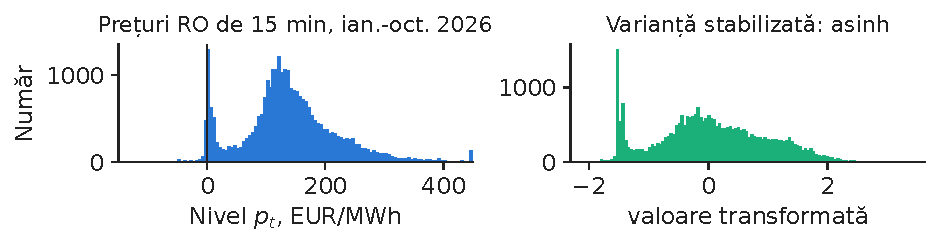
\includegraphics[width=\textwidth,height=0.386\textheight,keepaspectratio]{charts/ro/asinh_ro.pdf}\end{center}\vspace{-3mm}
\chartsource{Sursa: energy-charts.info (Fraunhofer ISE); prețurile burselor OPCOM, IBEX, HUPX, EPEX SPOT, prin ENTSO-E. Date: toate intervalele de 15 min, 2026-01-01 - 2026-10-31.}
\vspace{0.5mm}
\begin{itemize}\setlength{\itemsep}{0pt}
  \item $\tilde p$ = mediana, $\widehat{\mathrm{MAD}}$ = abaterea absolută mediană (MAD) $\times1{,}4826$.
  \item ian.--oct. 2026: 1\,189 din 29\,184 de sferturi de oră cu preț $\le 0$ (502 exact 0)
    \begin{itemize}\setlength{\itemsep}{0pt}
      \item Asimetria 1{,}19 $\to$ 0{,}13, excesul de aplatizare (kurtosis) 6{,}73 $\to$ \ensuremath{-}0{,}55.
    \end{itemize}
\end{itemize}
\par\vfill\noindent{\scriptsize\color{FooterGray}(Uniejewski, Weron \& Ziel, 2018, IEEE TPWRS)}\hfill\qlink{EMQA\_L1\_asinh\_ro}{Quantlets/L1/EMQA_L1_asinh_ro}\par\vspace{0.5mm}
\end{frame}

\begin{frame}{Cozi groase: variațiile extreme ale țițeiului sînt mult mai frecvente}
\small
\intuition{„Cozi groase”: zilele cu variații foarte mari apar mult mai des decît permite clopotul lui Gauss.}
\begin{center}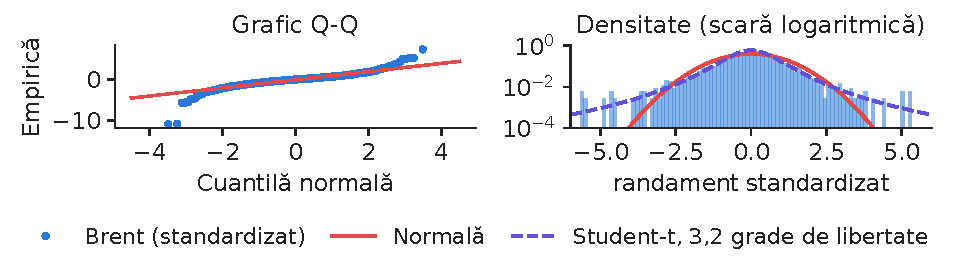
\includegraphics[width=\textwidth,height=0.398\textheight,keepaspectratio]{charts/ro/tails_brent.pdf}\end{center}\vspace{-3mm}
\chartsource{Sursa: Yahoo Finance (BZ=F). Date: 2015-01-05 - 2026-10-30.}
\vspace{0.5mm}
\begin{itemize}\setlength{\itemsep}{0pt}
  \item Randamente logaritmice zilnice Brent, fără cele 141 de zile de schimbare a contractului
    \begin{itemize}\setlength{\itemsep}{0pt}
      \item Peste 4 abateri standard: 16 observate, 0{,}18 așteptate sub normalitate, exces de aplatizare (kurtosis) 13{,}98 (testul Jarque--Bera (JB): Anexa F).
    \end{itemize}
\end{itemize}
\par\vfill\manager{un buget de combustibil bazat pe legea normală subestimează zilele de criză (cursul 4).}\par\vspace{0.5mm}
\par\vfill\noindent{\scriptsize\color{FooterGray}(Jarque \& Bera, 1980, Econ.\ Letters; Yahoo Finance BZ=F)}\hfill\qlink{EMQA\_L1\_tails\_brent}{Quantlets/L1/EMQA_L1_tails_brent}\par\vspace{0.5mm}
\end{frame}

\begin{frame}{Perioadele calme și cele agitate apar grupat}
\small
\intuition{O variație mare azi face probabilă o altă variație mare, indiferent de sens.}
\vspace{-1mm}\[ Q(m)=T(T+2)\sum_{k=1}^{m}\frac{\hat\rho_k^2}{T-k}\ \sim\ \chi^2_m\quad\text{(Ljung--Box)} \]\vspace{-2mm}
\begin{center}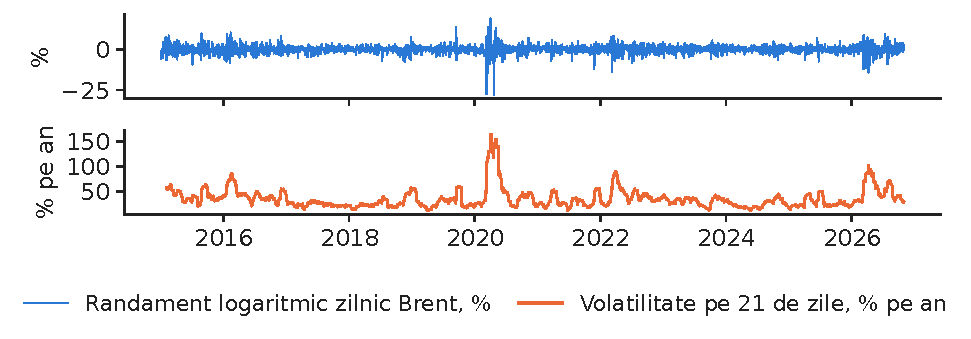
\includegraphics[width=\textwidth,height=0.358\textheight,keepaspectratio]{charts/ro/volclust_brent.pdf}\end{center}\vspace{-3mm}
\chartsource{Sursa: Yahoo Finance (BZ=F). Date: 2015-01-05 - 2026-10-30.}
\vspace{0.5mm}
\begin{itemize}\setlength{\itemsep}{0pt}
  \item Brent: $Q_{10}(r)=$ 28{,}1, dar $Q_{10}(r^2)=$ 506{,}9 (valoarea critică la 5\%: 18{,}31)
    \begin{itemize}\setlength{\itemsep}{0pt}
      \item Memorie slabă pentru sensul variațiilor, puternică pentru mărimea lor.
    \end{itemize}
\end{itemize}
\par\vfill\manager{după un șoc, limitele de risc rămîn mai largi săptămîni, nu zile (cursul 3).}\par\vspace{0.5mm}
\par\vfill\noindent{\scriptsize\color{FooterGray}(Ljung \& Box, 1978, Biometrika)}\hfill\qlink{EMQA\_L1\_volclust\_brent}{Quantlets/L1/EMQA_L1_volclust_brent}\par\vspace{0.5mm}
\end{frame}


\section{Instrumente de analiză a seriilor de timp}

\subsection{Staționaritate și autocorelație}

\begin{frame}{Staționaritate: regulile jocului nu se schimbă în timp}
\small
\intuition{Slab staționară: media, dispersia și memoria la fiecare decalaj $k$ sînt aceleași în orice perioadă.}
\vspace{-1mm}\[ \E X_t=\mu,\quad \Var X_t=\gamma_0,\quad \Cov(X_t,X_{t-k})=\gamma_k\quad \text{pentru orice } t \]\vspace{-2mm}
\begin{center}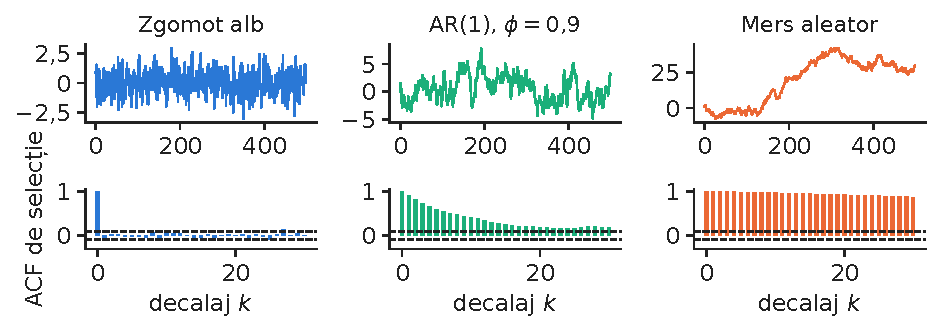
\includegraphics[width=\textwidth,height=0.397\textheight,keepaspectratio]{charts/ro/sim_wn_ar_rw.pdf}\end{center}\vspace{-3mm}
\chartsource{\simlabel\ Sursa: simulare, numpy, seed = 20261104. Date: T = 500, șocuri N(0,1).}
\vspace{0.5mm}
\begin{itemize}\setlength{\itemsep}{0pt}
  \item Zgomot alb, un model autoregresiv (AR) de ordinul 1, AR(1), cu $\phi=0{,}9$, un mers aleator
    \begin{itemize}\setlength{\itemsep}{0pt}
      \item AR(1) revine la medie; șocurile mersului aleator sînt permanente: autocorelația 0{,}96 la decalajul 10
    \end{itemize}
\end{itemize}
\par\vfill\manager{un preț mediu istoric este o prognoză numai dacă seria este staționară.}\par\vspace{0.5mm}
\par\vfill\noindent{\scriptsize\color{FooterGray}(Hyndman \& Athanasopoulos, 2021, OTexts)}\hfill\qlink{EMQA\_L1\_sim\_wn\_ar\_rw}{Quantlets/L1/EMQA_L1_sim_wn_ar_rw}\par\vspace{0.5mm}
\end{frame}

\begin{frame}{Autocorelația: cît din trecut se regăsește în prețul de azi}
\footnotesize
\intuition{Autocorelația de ordinul $k$ este corelația dintre serie și aceeași serie decalată cu $k$ perioade.}
\begin{columns}[T,onlytextwidth]
\begin{column}{0.52\textwidth}
\[ \hat\rho_k=\frac{\sum_{t=k+1}^{T}(x_t-\bar x)(x_{t-k}-\bar x)}{\sum_{t=1}^{T}(x_t-\bar x)^2} \]\begin{itemize}\setlength{\itemsep}{1pt}
  \item Banda de încredere pentru zgomot alb: $\pm1{,}96/\sqrt T$.
  \item Banda Bartlett la decalajul $k$: $\pm1{,}96\sqrt{(1+2\sum_{j<k}\hat\rho_j^2)/T}$, valabilă dacă autocorelația teoretică este nulă după decalajul $k-1$.
  \item Funcția de autocorelație parțială (PACF): memoria la decalajul $k$, după eliminarea efectului decalajelor mai mici.
\end{itemize}
\end{column}
\begin{column}{0.45\textwidth}
\begin{itemize}\setlength{\itemsep}{1pt}
  \item \textbf{Patru reguli de interpretare}
    \begin{itemize}\setlength{\itemsep}{0pt}
      \item Scădere lentă de la valori apropiate de 1: persistență sau rădăcină unitară; testați
      \item Scădere geometrică, PACF se anulează după $p$ decalaje: un model AR($p$)
      \item Vîrfuri la decalajele 7, 14 (zile) sau 24, 168 (ore): sezonalitate
      \item Toate valorile în bandă: nicio memorie liniară (verificați și $x_t^2$)
    \end{itemize}
\end{itemize}
\end{column}
\end{columns}
\par\vfill\manager{prognoza unui furnizor pentru ziua de mîine pornește de la „aceeași zi din săptămîna trecută”: $\hat\rho_7=$ 0{,}672 în România, din 2023.}\par\vspace{0.5mm}
\par\vfill\noindent{\scriptsize\color{FooterGray}(Hyndman \& Athanasopoulos, 2021; Ljung \& Box, 1978)}\hfill\tryit{notebook-ul Jupyter \S6}\par\vspace{0.5mm}
\end{frame}

\begin{frame}{Prețul ține minte ziua de ieri, săptămîna trecută și aceeași oră}
\small
\begin{center}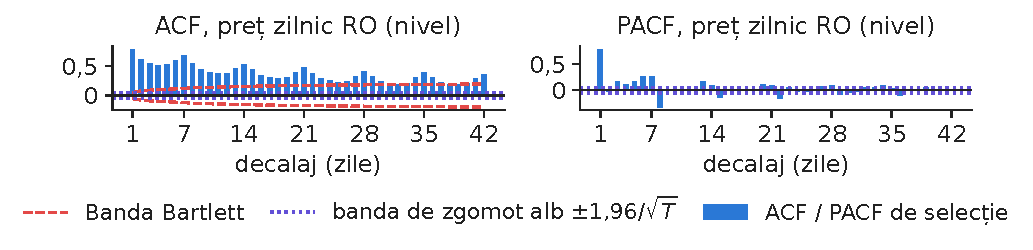
\includegraphics[width=\textwidth,height=0.371\textheight,keepaspectratio]{charts/ro/acf_pacf_ro_daily.pdf}\end{center}\vspace{-3mm}

\begin{center}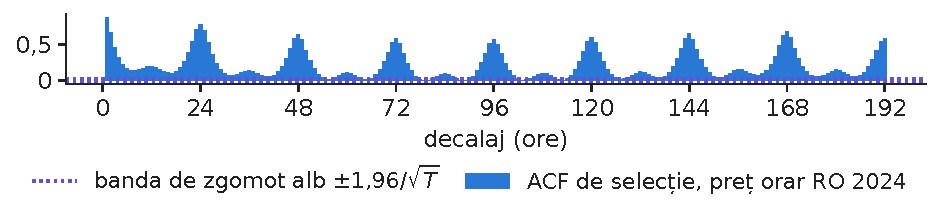
\includegraphics[width=\textwidth,height=0.251\textheight,keepaspectratio]{charts/ro/acf_ro_hourly.pdf}\end{center}\vspace{-3mm}
\chartsource{Sursa: energy-charts.info (Fraunhofer ISE); prețurile burselor OPCOM, IBEX, HUPX, EPEX SPOT, prin ENTSO-E. Date: sus: 2023-01-01 - 2026-10-31, T = 1400; jos: 2024, date orare, T = 8784.}
\begin{itemize}\setlength{\itemsep}{1pt}
  \item Date zilnice, 1 ianuarie 2023 -- 31 octombrie 2026: $\hat\rho_1=$ 0{,}789, $\hat\rho_7=$ 0{,}672, PACF $\hat\alpha_7=$ 0{,}257
    \begin{itemize}\setlength{\itemsep}{0pt}
      \item Date orare, 2024: $\hat\rho_{24}=$ 0{,}776, $\hat\rho_{168}=$ 0{,}681.
    \end{itemize}
\end{itemize}
\par\vfill\noindent{\scriptsize\color{FooterGray}(Ziel \& Weron, 2018, ENEECO)}\hfill\qlink{EMQA\_L1\_acf\_pacf\_ro\_daily}{Quantlets/L1/EMQA_L1_acf_pacf_ro_daily}\hspace{0.8em}\qlink{EMQA\_L1\_acf\_ro\_hourly}{Quantlets/L1/EMQA_L1_acf_ro_hourly}\par\vspace{0.5mm}
\end{frame}

\begin{frame}{Prognoza naivă: reperul pe care orice model trebuie să-l depășească}
\small
\intuition{Mîine, fiecare oră costă cît a costat azi (după weekend: ca săptămîna trecută).}
\vspace{-1mm}\[ \hat p_{d,h}=\begin{cases} p_{d-1,h} & d=\text{Ma--Vi}\\ p_{d-7,h} & d=\text{Lu, Sî, Du}\end{cases},\qquad \mathrm{MAE}=\frac{1}{n}\sum_{d,h}|p_{d,h}-\hat p_{d,h}| \]\vspace{-2mm}
\begin{center}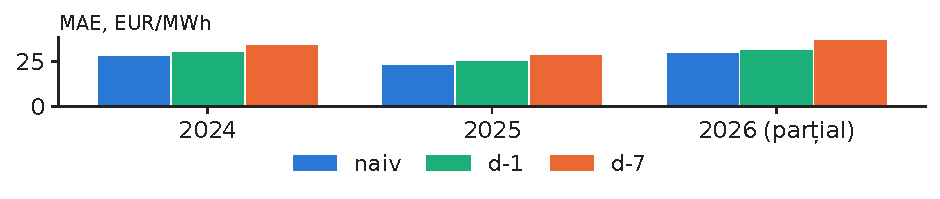
\includegraphics[width=\textwidth,height=0.302\textheight,keepaspectratio]{charts/ro/naive_bar.pdf}\end{center}\vspace{-3mm}
\chartsource{Sursa: energy-charts.info (Fraunhofer ISE); prețurile burselor OPCOM, IBEX, HUPX, EPEX SPOT, prin ENTSO-E. Date: prețuri PZU orare, 2024-01 - 2026-10.}
\vspace{0.5mm}
\begin{itemize}\setlength{\itemsep}{0pt}
  \item Eroarea absolută medie (MAE), România, 2025: 22{,}9 EUR/MWh, la un preț mediu de 108{,}2
    \begin{itemize}\setlength{\itemsep}{0pt}
      \item Regula zi lucrătoare/weekend bate ambele decalaje simple în 7 din 8 ani (Anexa E).
    \end{itemize}
\end{itemize}
\par\vfill\manager{înainte de a plăti un serviciu de prognoză, cereți-i MAE alături de acest reper.}\par\vspace{0.5mm}
\par\vfill\noindent{\scriptsize\color{FooterGray}(Nogales et al., 2002, IEEE TPWRS; Weron, 2014, IJF; Lago et al., 2021, APEN)}\hfill\qlink{EMQA\_L1\_naive\_bar}{Quantlets/L1/EMQA_L1_naive_bar}\par\vspace{0.5mm}
\end{frame}

\subsection{Teste de rădăcină unitară, descompunere și netezire}

\begin{frame}{Persistența șocurilor: două teste cu ipoteze opuse}
\footnotesize
\intuition{Un test pornește de la ipoteza „șocurile sînt permanente” și caută o revenire la medie; celălalt pornește de la „seria este stabilă” și caută o derivă lentă.}
\begin{columns}[T,onlytextwidth]
\begin{column}{0.55\textwidth}
\[ \Delta x_t=\alpha+\underbrace{\gamma\,x_{t-1}}_{\text{revenirea la medie}}+\underbrace{\textstyle\sum_{j}\delta_j\Delta x_{t-j}}_{\text{decalaje}}+u_t \]{\footnotesize\begin{itemize}\setlength{\itemsep}{0pt}
  \item \textbf{\txtwhere}
    \begin{itemize}\setlength{\itemsep}{0pt}
      \item Testul Dickey--Fuller augmentat (ADF): $H_0:\gamma=0$ (rădăcină unitară), $\hat\gamma/\mathrm{se}$ comparat cu valorile critice Dickey--Fuller (circa $-2{,}86$ la 5\%), decalajele $p$ alese după criteriul informațional Akaike (AIC)
      \item Testul Kwiatkowski--Phillips--Schmidt--Shin (KPSS): $H_0$ = serie staționară, respinsă la valori mari (0{,}463 la 5\%)
      \item Formulele complete: Anexa A.
    \end{itemize}
\end{itemize}\par}
\end{column}
\begin{column}{0.42\textwidth}
{\scriptsize\renewcommand{\arraystretch}{1.05}\setlength{\tabcolsep}{4pt}
\begin{tabular}{@{}lll@{}}\toprule
$H_0$: & KPSS nerespinsă & KPSS respinsă \\ \midrule
ADF respinsă & \cellcolor{Forest!25}staționar & \cellcolor{Bitter!30}conflict \\
ADF nerespinsă & neconcludent & \cellcolor{Crimson!25}răd.\ unitară$^{*}$ \\
\bottomrule\end{tabular}}\par\vspace{1mm}\begin{itemize}\setlength{\itemsep}{1pt}
  \item $^{*}$Compatibil cu o rădăcină unitară, dar nu este o dovadă: testul ADF are putere redusă în cazul revenirii lente la medie, iar rupturile de nivel (2022) favorizează nerespingerea rădăcinii unitare.
\end{itemize}
\end{column}
\end{columns}
\par\vfill\manager{dacă șocurile pot fi permanente, un furnizor nu își poate baza bugetul pe „revenirea la normal”.}\par\vspace{0.5mm}
\par\vfill\noindent{\scriptsize\color{FooterGray}(Dickey \& Fuller, 1979, JASA; Kwiatkowski et al., 1992, J.\ Econometrics)}\hfill\tryit{notebook-ul Jupyter \S7}\par\vspace{0.5mm}
\end{frame}

\begin{frame}{Un verdict pe serie: nivelurile persistă, variațiile sînt staționare}
\small
{\footnotesize\renewcommand{\arraystretch}{1.0}\setlength{\tabcolsep}{4pt}
\begin{tabular}{@{}llrrrrrl@{}}\toprule
Seria & Perioada & $T$ & ADF & $p$ & KPSS & $p$ & Verdict \\ \midrule
Preț RO, nivel & 2015--2026 & 4\,317 & \ensuremath{-}2{,}71 & 0{,}073 & 3{,}645 & $<$0{,}01 & \cellcolor{Crimson!25}rădăcină unitară$^{*}$ \\
Preț RO, variație zilnică & 2015--2026 & 4\,312 & \ensuremath{-}14{,}81 & $<$0{,}001 & 0{,}045 & $>$0{,}10 & \cellcolor{Forest!25}staționar \\
Preț DE-LU, nivel & 2015--2026 & 4\,322 & \ensuremath{-}3{,}54 & 0{,}007 & 3{,}441 & $<$0{,}01 & \cellcolor{Bitter!30}conflict \\
Brent, logaritmul prețului & 2015--2026 & 2\,976 & \ensuremath{-}2{,}19 & 0{,}212 & 3{,}820 & $<$0{,}01 & \cellcolor{Crimson!25}rădăcină unitară$^{*}$ \\
Brent, randament logaritmic & 2015--2026 & 2\,975 & \ensuremath{-}10{,}79 & $<$0{,}001 & 0{,}049 & $>$0{,}10 & \cellcolor{Forest!25}staționar \\
Hidro RO, desezonalizat & 2015--2025 & 132 & \ensuremath{-}4{,}19 & $<$0{,}001 & 0{,}354 & 0{,}097 & \cellcolor{Forest!25}staționar \\
\bottomrule\end{tabular}}
\par\vspace{0.5mm}{\scriptsize \begin{itemize}\setlength{\itemsep}{0pt}
  \item $^{*}$Compatibil cu o rădăcină unitară (ipoteză nerespinsă); nu este o dovadă.
\end{itemize}}
\vspace{1mm}
\begin{itemize}\setlength{\itemsep}{1pt}
  \item \textbf{Nivelurile} RO și Brent sînt compatibile cu o rădăcină unitară, \textbf{variațiile} sînt staționare.
  \item Germania: ambele teste își resping ipoteza nulă (conflict): revenire la medie și saltul de nivel din 2021--2022.
  \item Seria hidro este testată după scăderea mediilor lunare (serie sezonieră)
    \begin{itemize}\setlength{\itemsep}{0pt}
      \item Prețul din România numai din 2023: ADF $p=$ 0{,}361, KPSS 1{,}039.
    \end{itemize}
\end{itemize}
\par\vfill\manager{modelați \emph{variațiile} prețului (sau prețul transformat) și includeți explicit sezonalitatea.}\par\vspace{0.5mm}
\par\vfill\noindent{\scriptsize\color{FooterGray}(calcule proprii; numai constantă; decalaje ADF după AIC; prag de 5\%)}\hfill\tryit{notebook-ul Jupyter \S7}\par\vspace{0.5mm}
\end{frame}

\begin{frame}{Descompunerea: trend, sezonalitate și componenta reziduală}
\small
\intuition{Descompunerea sezonieră și de trend prin regresie locală (STL) lasă sezonul să evolueze.}
\vspace{-1mm}\[ x_t=T_t+S_t+R_t\qquad(\text{trend + sezon + rest}) \]\vspace{-2mm}
\begin{center}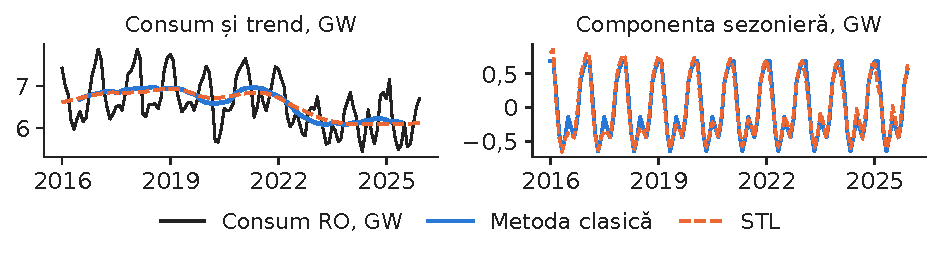
\includegraphics[width=\textwidth,height=0.363\textheight,keepaspectratio]{charts/ro/decomp_load.pdf}\end{center}\vspace{-3mm}
\chartsource{Sursa: energy-charts.info (Fraunhofer ISE); ENTSO-E (date Transelectrica pentru România). Date: 2016-01 - 2025-12, consum mediu lunar.}
\vspace{0.5mm}
\begin{itemize}\setlength{\itemsep}{0pt}
  \item Consumul României față de trend: ian. \ensuremath{+}0{,}69, feb. \ensuremath{+}0{,}69, mai \ensuremath{-}0{,}65 GW
    \begin{itemize}\setlength{\itemsep}{0pt}
      \item Amplitudinea STL: 1{,}52 $\to$ 1{,}27 GW, ponderile mediei mobile (MA): Anexa B.
    \end{itemize}
\end{itemize}
\par\vfill\manager{Transelectrica și furnizorii planifică lunar capacitățile cu indici sezonieri.}\par\vspace{0.5mm}
\par\vfill\noindent{\scriptsize\color{FooterGray}(Cleveland et al., 1990, JOS; Hyndman \& Athanasopoulos, 2021)}\hfill\qlink{EMQA\_L1\_decomp\_load}{Quantlets/L1/EMQA_L1_decomp_load}\par\vspace{0.5mm}
\end{frame}

\begin{frame}{Netezirea exponențială: datele recente cîntăresc mai mult}
\small
\intuition{Nivelul netezit: medie ponderată a valorilor trecute, cu ponderi care scad geometric.}
\vspace{-1mm}\[ \ell_t=\underbrace{\alpha x_t}_{\text{informația nouă}}+\underbrace{(1-\alpha)\ell_{t-1}}_{\text{memoria}},\qquad \alpha=1-2^{-1/h} \]\vspace{-2mm}
\begin{center}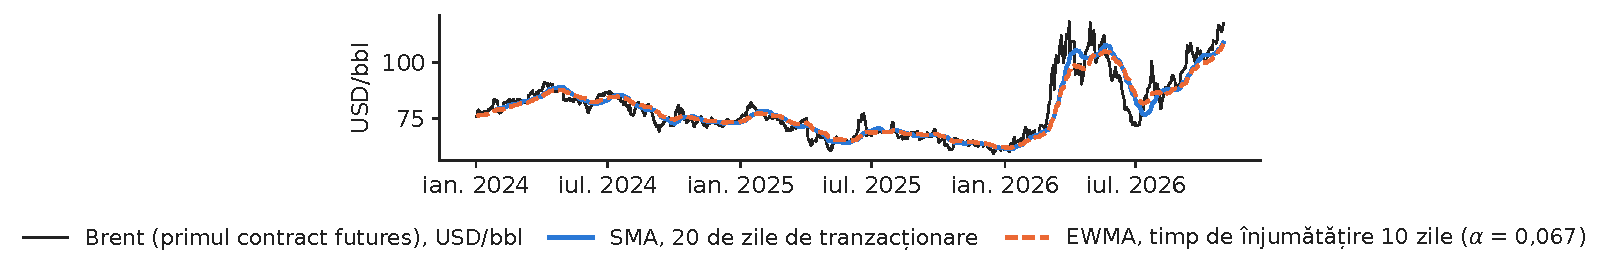
\includegraphics[width=\textwidth,height=0.378\textheight,keepaspectratio]{charts/ro/smooth_brent.pdf}\end{center}\vspace{-3mm}
\chartsource{Sursa: Yahoo Finance (BZ=F). Date: 2024-01-02 - 2026-10-30.}
\vspace{0.5mm}
\begin{itemize}\setlength{\itemsep}{0pt}
  \item $h$ = timpul de înjumătățire (zile), deci media mobilă ponderată exponențial (EWMA) are $\alpha=$ 0{,}067
    \begin{itemize}\setlength{\itemsep}{0pt}
      \item Ponderea optimă a netezirii exponențiale simple (SES): 0{,}948, practic ultimul preț.
    \end{itemize}
\end{itemize}
\par\vfill\manager{EWMA este un bun preț de referință în contracte, dar o prognoză slabă.}\par\vspace{0.5mm}
\par\vfill\noindent{\scriptsize\color{FooterGray}(Hyndman \& Athanasopoulos, 2021, OTexts, ch.\ 8)}\hfill\qlink{EMQA\_L1\_smooth\_brent}{Quantlets/L1/EMQA_L1_smooth_brent}\par\vspace{0.5mm}
\end{frame}


\section{Studii de caz pe date recente}

\subsection{(a) 2023, an ploios; 2025, an secetos}

\begin{frame}{Studiul de caz (a): producția hidro în 2025, cu o treime sub 2023}
\small
\begin{center}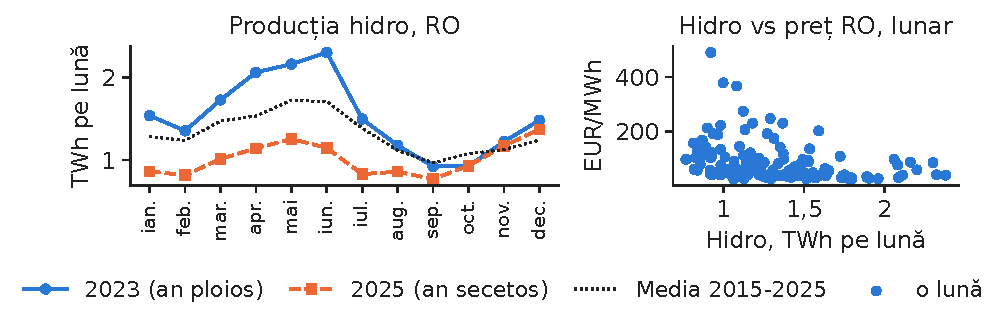
\includegraphics[width=\textwidth,height=0.471\textheight,keepaspectratio]{charts/ro/hydro_case.pdf}\end{center}\vspace{-3mm}
\chartsource{Sursa: energy-charts.info (Fraunhofer ISE); ENTSO-E (date Transelectrica pentru România). Date: lunar, 2015-01 - 2025-12.}
\vspace{0.5mm}
\begin{itemize}\setlength{\itemsep}{0pt}
  \item Hidro: 18{,}34 TWh în 2023 (maximul din 2015) și 12{,}15 TWh în 2025 (minimul), \textbf{\ensuremath{-}33{,}8\%}
    \begin{itemize}\setlength{\itemsep}{0pt}
      \item 2025 față de media 2015--2025 (15{,}85 TWh): \ensuremath{-}23{,}3\%.
    \end{itemize}
  \item România a trecut de la export net (\ensuremath{-}3{,}06 TWh) la import net (\ensuremath{+}3{,}76 TWh)
    \begin{itemize}\setlength{\itemsep}{0pt}
      \item Compatibil cu lipsa apei, dar s-au schimbat și nuclearul, cererea și prețurile vecinilor.
    \end{itemize}
\end{itemize}
\par\vfill\manager{producția unei companii hidro și factura unui importator net depind de ploaie.}\par\vspace{0.5mm}
\par\vfill\noindent{\scriptsize\color{FooterGray}(energy-charts.info; sursa datelor: ENTSO-E)}\hfill\qlink{EMQA\_L1\_hydro\_case}{Quantlets/L1/EMQA_L1_hydro_case}\par\vspace{0.5mm}
\end{frame}

\begin{frame}{Studiul de caz (a): mai multă apă, prețuri mai mici}
\footnotesize
\intuition{Cu gazele la preț fix, lunile cu mai multă apă au avut prețuri mai mici: o asociere, nu un efect cauzal.}
\begin{columns}[T,onlytextwidth]
\begin{column}{0.50\textwidth}
\[ p_m=\beta_0+\underbrace{\beta_1\,\mathrm{Hydro}_m}_{\text{apa}}+\underbrace{\beta_2\,\mathrm{TTF}_m}_{\text{costul gazelor}}+u_m \]{\footnotesize\begin{itemize}\setlength{\itemsep}{0pt}
  \item \textbf{\txtwhere}
    \begin{itemize}\setlength{\itemsep}{0pt}
      \item $p_m$ = prețul mediu PZU în luna $m$ (EUR/MWh)
      \item $\mathrm{Hydro}_m$ = producția hidro (TWh)
      \item $\mathrm{TTF}_m$ = prețul gazelor pe hubul olandez (EUR/MWh)
      \item Estimare prin metoda celor mai mici pătrate (OLS), cu erori standard robuste la heteroscedasticitate și autocorelație (HAC), 6 decalaje.
    \end{itemize}
\end{itemize}\par}
\end{column}
\begin{column}{0.47\textwidth}
{\footnotesize\renewcommand{\arraystretch}{1.05}\setlength{\tabcolsep}{4pt}
\begin{tabular}{@{}lrrr@{}}\toprule
2015--2025 & $\hat\beta$ & e.s. & $t$ \\ \midrule
Constantă & 44{,}80 & 10{,}21 & 4{,}39 \\
Hydro & \ensuremath{-}19{,}55 & 7{,}02 & \ensuremath{-}2{,}78 \\
TTF & 1{,}89 & 0{,}06 & 34{,}16 \\
\bottomrule\end{tabular}}\par\vspace{1mm}\begin{itemize}\setlength{\itemsep}{1pt}
  \item Un TWh hidro în plus într-o lună: în medie, \ensuremath{-}19{,}55 EUR/MWh, la același preț al gazelor.
  \item Atenție: prețurile energiei și ale gazelor au trend (secțiunea 3), deci fără cointegrare regresia poate fi spurioasă
    \begin{itemize}\setlength{\itemsep}{0pt}
      \item $R^2=$ 0{,}941 nu este o dovadă
      \item Cointegrarea se testează în cursul 2.
    \end{itemize}
\end{itemize}
\end{column}
\end{columns}
\par\vfill\manager{producătorii hidro și traderii urmăresc nivelul lacurilor ca indicator anticipativ al prețului PZU.}\par\vspace{0.5mm}
\par\vfill\noindent{\scriptsize\color{FooterGray}(estimare proprie; erori standard Newey--West)}\hfill\tryit{notebook-ul Jupyter \S10a}\par\vspace{0.5mm}
\end{frame}

\subsection{(b) Șocul petrolier din iunie 2025}

\begin{frame}{Studiul de caz (b): Brent, +7\% într-o zi, apoi sub nivelul inițial}
\small
\begin{center}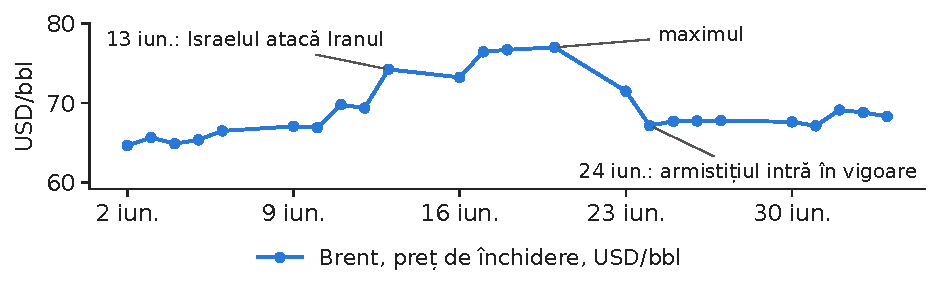
\includegraphics[width=\textwidth,height=0.416\textheight,keepaspectratio]{charts/ro/iran_brent.pdf}\end{center}\vspace{-3mm}
\chartsource{Sursa: Yahoo Finance (BZ=F). Date: 2025-06-02 - 2025-07-04, zile de tranzacționare.}
\vspace{0.5mm}
\begin{itemize}\setlength{\itemsep}{0pt}
  \item Prețul de închidere: 12 iunie 2025 69{,}36 $\to$ 13 iunie (Israelul atacă Iranul) 74{,}23, adică \textbf{\ensuremath{+}7{,}0\%} (4{,}3 abateri standard ale randamentelor zilnice din 2024)
    \begin{itemize}\setlength{\itemsep}{0pt}
      \item Maximul: 77{,}01, la 20 iunie 2025
      \item 24 iunie, cu armistițiul în vigoare: 67{,}14, adică \textbf{\ensuremath{-}12{,}8\%} față de maxim și \ensuremath{-}3{,}2\% față de 12 iunie.
    \end{itemize}
\end{itemize}
\par\vfill\manager{un cumpărător de combustibil și-a acoperit riscul la maximul din 20 iunie
    \begin{itemize}\setlength{\itemsep}{0pt}
      \item Patru zile mai tîrziu, piața era mult sub prețul fixat.
    \end{itemize}}\par\vspace{0.5mm}
\par\vfill\noindent{\scriptsize\color{FooterGray}(Yahoo Finance, Brent BZ=F)}\hfill\qlink{EMQA\_L1\_iran\_brent}{Quantlets/L1/EMQA_L1_iran_brent}\par\vspace{0.5mm}
\end{frame}

\subsection{(c) Separarea regională a prețurilor în vara lui 2024}

\begin{frame}{Studiul de caz (c): în iulie 2024, România a plătit dublul prețului din Germania}
\small
\begin{center}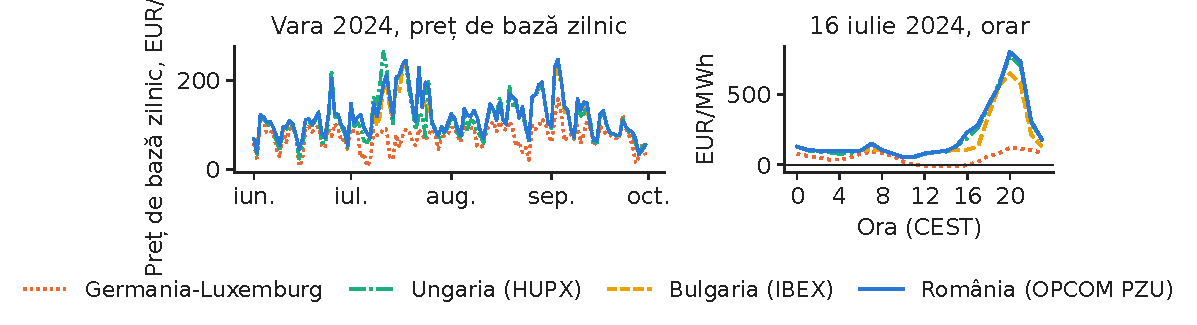
\includegraphics[width=\textwidth,height=0.439\textheight,keepaspectratio]{charts/ro/separation_2024.pdf}\end{center}\vspace{-3mm}
\chartsource{Sursa: energy-charts.info (Fraunhofer ISE); prețurile burselor OPCOM, IBEX, HUPX, EPEX SPOT, prin ENTSO-E. Date: 2024-06-01 - 2024-09-30 zilnic (stînga); 2024-07-16 orar (dreapta).}
\vspace{0.5mm}
\begin{itemize}\setlength{\itemsep}{0pt}
  \item Mediile din iulie 2024: RO 145{,}14, BG 136{,}47, HU 135{,}54, DE-LU 67{,}70 EUR/MWh
    \begin{itemize}\setlength{\itemsep}{0pt}
      \item 16 iulie: diferența RO--DE-LU, 162{,}87
      \item Vîrful orar din România, 801{,}62 la ora 20:00, în timp ce DE-LU avea \ensuremath{-}11{,}48 la ora 14:00.
    \end{itemize}
\end{itemize}
\par\vfill\manager{pentru cumpărătorii din sud-estul Europei, serile verilor caniculare și secetoase reprezintă principalul risc de preț.}\par\vspace{0.5mm}
\par\vfill\noindent{\scriptsize\color{FooterGray}(energy-charts.info; prețuri PZU zilnice și orare)}\hfill\qlink{EMQA\_L1\_separation\_2024}{Quantlets/L1/EMQA_L1_separation_2024}\par\vspace{0.5mm}
\end{frame}

\begin{frame}{Studiul de caz (c): seri caniculare și o rețea congestionată}
\small
\begin{columns}[T,onlytextwidth]
\begin{column}{0.60\textwidth}
\begin{itemize}\setlength{\itemsep}{1pt}
  \item Prețuri egale (diferență sub 0{,}01 EUR/MWh) în orele din iulie: RO--BG 86{,}8\%, RO--HU 6{,}3\%, RO--DE-LU 3{,}1\%
    \begin{itemize}\setlength{\itemsep}{0pt}
      \item Rețeaua spre Europa Centrală era la limita capacității
      \item Elementul de rețea saturat nu poate fi identificat numai din prețuri.
    \end{itemize}
  \item După apus, producția solară dispare, iar aerul condiționat menține cererea ridicată
    \begin{itemize}\setlength{\itemsep}{0pt}
      \item Regiunea trebuie să importe exact atunci.
    \end{itemize}
  \item Producția hidro în iulie--august: 1{,}94 TWh în 2024, față de 2{,}67 TWh în 2023
    \begin{itemize}\setlength{\itemsep}{0pt}
      \item Importul net mediu: 737 MW, față de 66 MW.
    \end{itemize}
  \item Vîrful verii: prețul zilnic din România, 246{,}89 EUR/MWh, la 3 septembrie 2024 (DE-LU 158{,}39)
    \begin{itemize}\setlength{\itemsep}{0pt}
      \item Prețul orar, 1021{,}61 la ora 19:00 CEST, cel mai mare preț orar din România în datele noastre.
    \end{itemize}
\end{itemize}
\end{column}
\begin{column}{0.37\textwidth}
\begin{block}{Concluzii pentru modelare}
\begin{itemize}\setlength{\itemsep}{1pt}
  \item Prețurile piețelor cuplate sînt egale numai cît timp rețeaua nu este la limită.
  \item Modelați prețul din România cu factori regionali: hidro, solar, consumul din sud-estul Europei.
  \item Tratați diferența față de Germania ca variabilă separată, dependentă de regim.
\end{itemize}
\end{block}
\end{column}
\end{columns}
\par\vfill\noindent{\scriptsize\color{FooterGray}(energy-charts.info; fluxuri fizice ENTSO-E)}\hfill\tryit{notebook-ul Jupyter \S10c}\par\vspace{0.5mm}
\end{frame}

\subsection{(d) Prețurile negative și energia solară}

\begin{frame}{Studiul de caz (d): prețurile negative apar mai ales primăvara}
\small
\begin{center}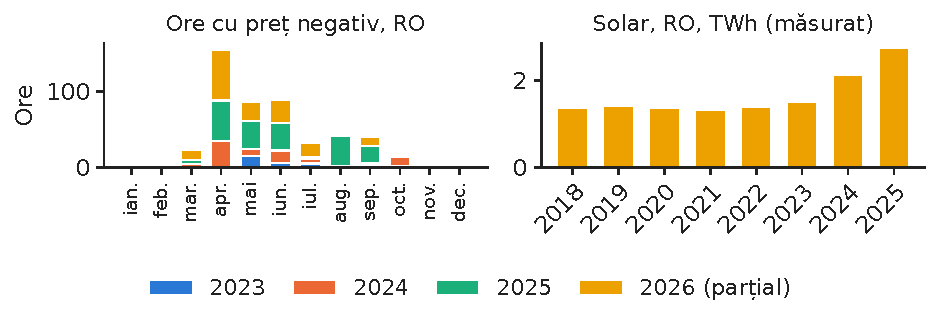
\includegraphics[width=\textwidth,height=0.422\textheight,keepaspectratio]{charts/ro/negative_solar.pdf}\end{center}\vspace{-3mm}
\chartsource{Sursa: energy-charts.info (Fraunhofer ISE); prețurile burselor OPCOM, IBEX, HUPX, EPEX SPOT, prin ENTSO-E. Date: ian. 2023 - 2026-10-31 (stînga); 2018-2025 (dreapta).}
\vspace{0.5mm}
\begin{itemize}\setlength{\itemsep}{0pt}
  \item Din 2023, lunile aprilie și mai concentrează 49{,}6\% din orele cu preț negativ din România (iunie--august: 34{,}0\%)
    \begin{itemize}\setlength{\itemsep}{0pt}
      \item Producția solară măsurată: 1{,}46 TWh (2023) $\to$ 2{,}72 TWh (2025), 4{,}33 TWh în ian.--oct. 2026.
    \end{itemize}
\end{itemize}
\par\vfill\manager{cele mai ieftine ore sînt cele de la amiază, în weekendurile de primăvară
    \begin{itemize}\setlength{\itemsep}{0pt}
      \item Atunci se încarcă bateriile, iar industria își poate programa consumul flexibil.
    \end{itemize}}\par\vspace{0.5mm}
\par\vfill\noindent{\scriptsize\color{FooterGray}(energy-charts.info; sursa datelor: ENTSO-E)}\hfill\qlink{EMQA\_L1\_negative\_solar}{Quantlets/L1/EMQA_L1_negative_solar}\par\vspace{0.5mm}
\end{frame}

\begin{frame}{Studiul de caz (d): factorii asociați zilelor cu prețuri negative}
\footnotesize
\intuition{Descriem condițiile efectiv înregistrate în zilele cu cel puțin un sfert de oră cu preț negativ; modelul descrie condițiile observate, fără a oferi prognoze pentru licitare.}
\begin{columns}[T,onlytextwidth]
\begin{column}{0.61\textwidth}
\[ \Pr(\text{zi negativă})=\Lambda\big(\beta_0+\underbrace{\beta_1R_d}_{\text{consum rezidual}}+\beta_2\mathrm{Hyd}_d+\underbrace{\beta_3\mathrm{Wkd}_d+\gamma_{y}}_{\text{calendar}}\big) \]{\footnotesize\begin{itemize}\setlength{\itemsep}{0pt}
  \item \textbf{\txtwhere}
    \begin{itemize}\setlength{\itemsep}{0pt}
      \item $\Lambda(u)=1/(1+e^{-u})$ (logit)
      \item Consumul rezidual $R_d$ = consum $-$ solar $-$ eolian (medii zilnice, GW), adică cererea rămasă pentru celelalte centrale
      \item $\gamma_y$ = efectele anuale
      \item Eșantionul: 1 ianuarie 2024 -- 31 octombrie 2026, $n=$ 1\,035 de zile, dintre care 108 cu prețuri negative
      \item Tabelul complet: Anexa F.
    \end{itemize}
\end{itemize}\par}
\end{column}
\begin{column}{0.36\textwidth}
\begin{itemize}\setlength{\itemsep}{1pt}
  \item \textbf{Interpretare}
    \begin{itemize}\setlength{\itemsep}{0pt}
      \item Fiecare GW în plus de consum rezidual înmulțește șansele unei zile cu prețuri negative cu 0{,}24
      \item Fiecare GW în plus de producție hidro înmulțește șansele cu 4{,}52
      \item O zi de weekend înmulțește șansele cu 16{,}13
      \item Pseudo-$R^2$ McFadden $=$ 0{,}369
    \end{itemize}
\end{itemize}
\end{column}
\end{columns}
\par\vfill\manager{regenerabilele sînt limitate cel mai probabil în weekendurile de primăvară, cu lacuri pline.}\par\vspace{0.5mm}
\par\vfill\noindent{\scriptsize\color{FooterGray}(estimare proprie, logit; energy-charts.info)}\hfill\tryit{notebook-ul Jupyter \S10d}\par\vspace{0.5mm}
\end{frame}

\subsection{(e) Anul 2026 pînă acum}

\begin{frame}{Studiul de caz (e): prețuri în creștere, saltul prețului țițeiului în martie}
\small
\begin{center}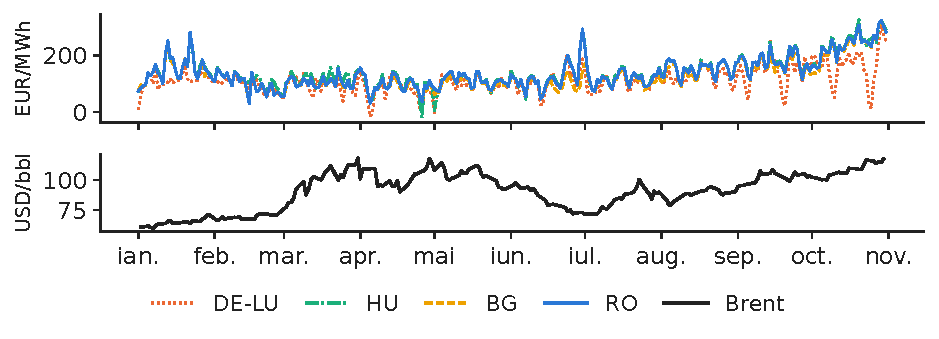
\includegraphics[width=\textwidth,height=0.433\textheight,keepaspectratio]{charts/ro/cy_prices.pdf}\end{center}\vspace{-3mm}
\chartsource{Sursa: energy-charts.info (prețurile burselor, prin ENTSO-E); Yahoo Finance (BZ=F). Date: 2026-01-01 - 2026-10-31, zilnic.}
\vspace{0.5mm}
\begin{itemize}\setlength{\itemsep}{0pt}
  \item ian.--oct. 2026: România 137{,}45 EUR/MWh (\ensuremath{+}29{,}8\%)
    \begin{itemize}\setlength{\itemsep}{0pt}
      \item În octombrie, 239{,}3, față de 121{,}9 cu un an înainte.
    \end{itemize}
  \item Media lunară Brent: 64{,}77 $\to$ 108{,}34 USD/bbl
    \begin{itemize}\setlength{\itemsep}{0pt}
      \item În martie, contractul pentru mai a crescut cu \ensuremath{+}52{,}2\% (presa: Iran, strîmtoarea Ormuz)
      \item \ensuremath{-}14{,}5\% la 1 aprilie: doar trecerea la contractul următor.
    \end{itemize}
\end{itemize}
\par\vfill\manager{bugetele stabilite în ianuarie s-au dovedit mult prea mici.}\par\vspace{0.5mm}
\par\vfill\noindent{\scriptsize\color{FooterGray}(energy-charts.info; Yahoo Finance BZ=F; date pînă la 31 octombrie 2026)}\hfill\qlink{EMQA\_L1\_cy\_prices}{Quantlets/L1/EMQA_L1_cy_prices}\par\vspace{0.5mm}
\end{frame}

\begin{frame}{Studiul de caz (e): Cernavodă oprită de două ori, hidro sub 2025}
\small
\begin{center}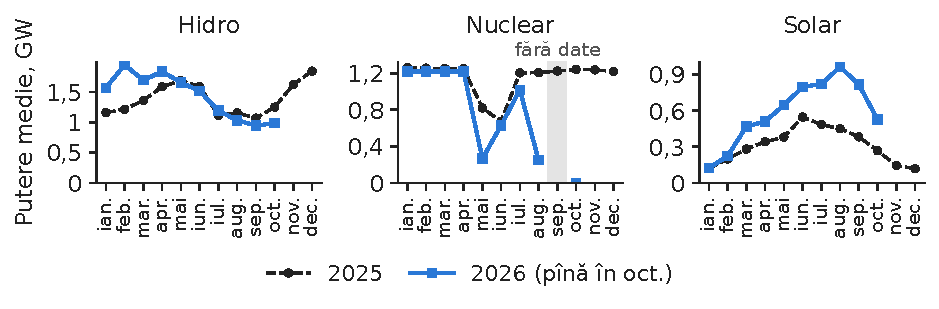
\includegraphics[width=\textwidth,height=0.466\textheight,keepaspectratio]{charts/ro/cy_generation.pdf}\end{center}\vspace{-3mm}
\chartsource{Sursa: energy-charts.info (Fraunhofer ISE); ENTSO-E (date Transelectrica pentru România). Date: medii lunare pe orele raportate, 2025-01 - 2026-10.}
\vspace{0.5mm}
\begin{itemize}\setlength{\itemsep}{0pt}
  \item Nuclear 0 MW în 19 zile din mai și din august (Dunărea scăzută)
    \begin{itemize}\setlength{\itemsep}{0pt}
      \item Ian.--oct.: \ensuremath{-}31{,}3\% pe orele raportate în ambii ani (limită inferioară).
    \end{itemize}
  \item Hidro \ensuremath{-}14{,}7\% în aug.--oct., solar \ensuremath{+}71{,}2\% de la începutul anului.
\end{itemize}
\par\vfill\manager{o singură centrală poate muta prețul național: citiți mesajele REMIT ca pe prognoza meteo.}\par\vspace{0.5mm}
\par\vfill\noindent{\scriptsize\color{FooterGray}(Nuclearelectrica, 29 iul. 2026; World Nuclear News, 30 iul. 2026; CNCAN, 9 sep. 2026)}\hfill\qlink{EMQA\_L1\_cy\_generation}{Quantlets/L1/EMQA_L1_cy_generation}\par\vspace{0.5mm}
\end{frame}

\begin{frame}{Studiul de caz (e): prețuri cu circa 30\% mai mari, ofertă mai mică}
\small
\begin{center}{\small\renewcommand{\arraystretch}{1.08}\setlength{\tabcolsep}{4pt}
\begin{tabular}{@{}lrrr@{}}\toprule
ian.--oct. & 2025 & 2026 & var. \% \\ \midrule
Preț RO, EUR/MWh & 105{,}88 & 137{,}45 & \cellcolor{Crimson!41}\ensuremath{+}29{,}8 \\
Preț DE-LU, EUR/MWh & 87{,}66 & 114{,}01 & \cellcolor{Crimson!41}\ensuremath{+}30{,}1 \\
RO $-$ DE-LU, EUR/MWh & 18{,}2 & 23{,}4 &  \\
Ore cu preț negativ, RO & 196 & 171{,}75 &  \\
Hidro RO, TWh & 9{,}61 & 10{,}44 & \cellcolor{Forest!12}\ensuremath{+}8{,}6 \\
Nuclear RO, TWh$^{*}$ & 7{,}42 & 5{,}10 & \cellcolor{Crimson!43}\ensuremath{-}31{,}3 \\
Solar RO, TWh & 2{,}53 & 4{,}33 & \cellcolor{Forest!55}\ensuremath{+}71{,}2 \\
Import net RO, TWh & 3{,}67 & 2{,}51 &  \\
\bottomrule\end{tabular}}\end{center}
\vspace{-3mm}
\par\vspace{0.5mm}{\scriptsize \begin{itemize}\setlength{\itemsep}{0pt}
  \item Verde = favorabil pentru consumator, roșu = nefavorabil; date pînă la 31 octombrie 2026.
  \item $^{*}$Numai orele raportate în ambii ani (limită inferioară).
\end{itemize}}
\par\vfill\manager{prețul a crescut cu circa 30\%, cu nuclearul, hidro și țițeiul în aceeași direcție, iar acoperirea riscului s-a dovedit rentabilă.}\par\vspace{0.5mm}
\par\vfill\noindent{\scriptsize\color{FooterGray}(calcule proprii; energy-charts.info)}\hfill\tryit{notebook-ul Jupyter \S10e}\par\vspace{0.5mm}
\end{frame}

\begin{frame}{Studiul de caz (e): valorile extreme din 2026, România și Brent}
\small
\begin{center}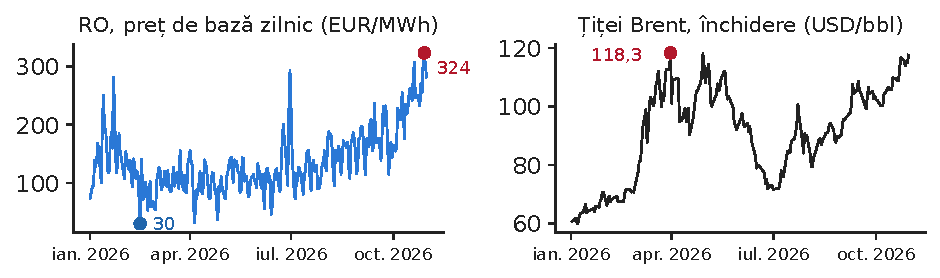
\includegraphics[width=\textwidth,height=0.550\textheight,keepaspectratio]{charts/ro/cy_extremes.pdf}\end{center}\vspace{-3mm}
\chartsource{Sursa: energy-charts.info (prețuri OPCOM); Yahoo Finance (BZ=F). Date: 2026-01-01 - 2026-10-31, zilnic.}
\vspace{0.5mm}
\begin{itemize}\setlength{\itemsep}{0pt}
  \item \textbf{România}
    \begin{itemize}\setlength{\itemsep}{0pt}
      \item Prețul de bază zilnic: maximul, 323{,}76 EUR/MWh, la 29 octombrie 2026; minimul, 29{,}63, la 15 februarie 2026
      \item Sfertul de oră: maximul, 1015{,}65, la 30 iunie 2026, ora 18:45; minimul, \ensuremath{-}99{,}75, la 26 aprilie 2026, ora 13:00 (CET/CEST)
    \end{itemize}
\end{itemize}
\par\vfill\noindent{\scriptsize\color{FooterGray}(calcule proprii; energy-charts.info; Yahoo Finance)}\hfill\qlink{EMQA\_L1\_cy\_extremes}{Quantlets/L1/EMQA_L1_cy_extremes}\par\vspace{0.5mm}
\end{frame}

\begin{frame}{Studiul de caz (e): valorile extreme din 2026, Germania și Brent}
\small
\begin{itemize}\setlength{\itemsep}{1pt}
  \item \textbf{Germania}
    \begin{itemize}\setlength{\itemsep}{0pt}
      \item Minimul pe sfert de oră: \ensuremath{-}499{,}99, la 1 mai 2026, ora 13:15, egal cu pragul de atunci
      \item După 26 aprilie și 1 mai, pragul a coborît la $-600$, din 29 mai 2026
    \end{itemize}
  \item \textbf{Țițeiul Brent}
    \begin{itemize}\setlength{\itemsep}{0pt}
      \item Cel mai mare preț de închidere: 118{,}35 USD/bbl, la 31 martie 2026
      \item Cea mai mare variație zilnică (fără schimbările de contract): \ensuremath{-}13{,}29\%, la 8 aprilie 2026
    \end{itemize}
\end{itemize}
\par\vfill\manager{stabiliți limitele de risc pe baza valorilor extreme, nu a mediilor.}\par\vspace{0.5mm}
\par\vfill\noindent{\scriptsize\color{FooterGray}(calcule proprii; nota SDAC a OPCOM, 7 mai 2026)}\hfill\tryit{notebook-ul Jupyter \S10e}\par\vspace{0.5mm}
\end{frame}

\subsection{(f) România, Bulgaria și bateriile}

\begin{frame}{Studiul de caz (f): din primăvara lui 2026, Bulgaria are prețuri mai mici seara}
\small
\begin{center}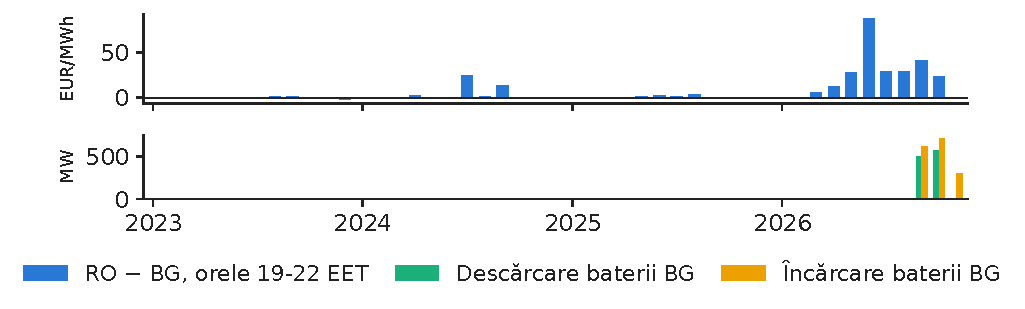
\includegraphics[width=\textwidth,height=0.354\textheight,keepaspectratio]{charts/ro/bg_battery.pdf}\end{center}\vspace{-3mm}
\chartsource{Sursa: energy-charts.info (Fraunhofer ISE); ENTSO-E (date Transelectrica pentru România). Date: 2023-01 - 2026-10, ora locală; seria bateriilor BG raportată din 2026-09-10.}
\vspace{0.5mm}
\begin{itemize}\setlength{\itemsep}{0pt}
  \item Seara, 19:00--22:00 ora locală (EET), apr.--sep., RO față de BG
    \begin{itemize}\setlength{\itemsep}{0pt}
      \item 171{,}1 față de 169{,}7 EUR/MWh (2025), 215{,}5 față de 178{,}0 (2026)
      \item La amiază (11:00--15:00), prețuri apropiate în 2026 (48{,}1 față de 46{,}0).
    \end{itemize}
  \item Datele despre baterii încep abia la 10 septembrie 2026, după apariția diferenței (mai 2026)
    \begin{itemize}\setlength{\itemsep}{0pt}
      \item Este o asociere, nu o dovadă.
    \end{itemize}
\end{itemize}
\par\vfill\manager{un dezvoltator român de stocare concurează pentru aceeași diferență de preț de seară (cursul 6).}\par\vspace{0.5mm}
\par\vfill\noindent{\scriptsize\color{FooterGray}(energy-charts.info; sursa datelor: ENTSO-E; calcule proprii, ora locală EET)}\hfill\qlink{EMQA\_L1\_bg\_battery}{Quantlets/L1/EMQA_L1_bg_battery}\par\vspace{0.5mm}
\end{frame}

\section*{Recapitulare}

\begin{frame}{Test 1: numărarea prețurilor negative}
\small
\begin{itemize}
  \item Într-o lună de după 1 octombrie 2025, 48 de prețuri pe sfert de oră din România au fost negative
    \begin{itemize}\setlength{\itemsep}{0pt}
      \item Un membru al consiliului de administrație vă întreabă cîte ore cu preț negativ au fost
      \item Ce îi răspundeți?
    \end{itemize}
\end{itemize}
\vspace{2mm}
\begin{exampleblock}{R\u{a}spuns}
\begin{itemize}
  \item $48\times15/60=12$ ore echivalente
    \begin{itemize}\setlength{\itemsep}{0pt}
      \item Dacă spuneți „48 de ore”, supraevaluați durata de 4 ori față de anii anteriori, cu intervale orare
      \item Formularea corectă: „48 de sferturi de oră (12 ore)”.
    \end{itemize}
\end{itemize}
\end{exampleblock}
\end{frame}

\begin{frame}{Test 2: citirea unei autocorelații}
\small
\begin{itemize}
  \item Un analist din echipa dumneavoastră afirmă: „autocorelația prețului PZU este 0{,}98 la decalajul 1 și 0{,}90 la decalajul 30, deci prețurile sînt zgomot alb, iar luna trecută nu ne spune nimic”
    \begin{itemize}\setlength{\itemsep}{0pt}
      \item Are dreptate?
    \end{itemize}
\end{itemize}
\vspace{2mm}
\begin{exampleblock}{R\u{a}spuns}
\begin{itemize}
  \item Nu: zgomotul alb are autocorelații apropiate de 0
    \begin{itemize}\setlength{\itemsep}{0pt}
      \item Valorile apropiate de 1 indică o persistență puternică, adică o rădăcină unitară sau o revenire foarte lentă la medie
      \item Aplicați testele ADF și KPSS și examinați autocorelația variațiilor zilnice.
    \end{itemize}
\end{itemize}
\end{exampleblock}
\end{frame}

\begin{frame}{Recapitulare}
\small
\vspace{-2mm}\begin{multicols}{2}\scriptsize\tableofcontents\end{multicols}
\begin{itemize}\setlength{\itemsep}{1pt}
  \item O singură licitație pe zi, cuplată la nivel european, cu 96 de sferturi de oră din oct. 2025
    \begin{itemize}\setlength{\itemsep}{0pt}
      \item Numărați în ore echivalente.
    \end{itemize}
  \item Reperul de depășit: prognoza naivă (România, 2025: MAE 22{,}92 EUR/MWh)
    \begin{itemize}\setlength{\itemsep}{0pt}
      \item Urmează prognoza (cursul 2).
    \end{itemize}
\end{itemize}
\end{frame}

\begin{frame}{Cercetările grupului nostru despre piața din România}
\footnotesize
\begin{itemize}\setlength{\itemsep}{1pt}
  \item \textbf{Criza din vara lui 2024} (studiul de caz c): analiză contrafactuală a crizei prețurilor din România din iunie--iulie 2024, pe date orare ENTSO-E
    \begin{itemize}\setlength{\itemsep}{0pt}
      \item Reducerea cererii cu 10\% este cea mai robustă dintre intervențiile prioritare, iar vîrful de preț s-a produs în ore aproape fără producție solară (Andrei, Pele \& Cramer, 2026, PICBE).
    \end{itemize}
  \item \textbf{Explicarea prognozelor de preț}: ce factori contează la fiecare orizont (de la 0--6 ore pînă la două săptămîni) și în fiecare regim de preț, pentru prețurile orare românești 2018--2024 (Andrei, Pele \& Cramer, 2026, PICBE) --- tema cursului 7.
  \item \textbf{Prognoza consumului național}: modele sezoniere clasice comparate cu rețele neuronale, pe consumul României (Proșcanu, Proșcanu, Pele \& Costea, 2025, Romanian J.\ Economic Forecasting) --- tema cursului 2.
  \item \textbf{Cererea abia reacționează la preț}: consumul din România este inelastic la preț
    \begin{itemize}\setlength{\itemsep}{0pt}
      \item Cauzalitatea în sens Granger merge de la consum la preț, nu invers (Proșcanu, Proșcanu \& Pele, 2025, J.\ Social and Economic Statistics) --- de aceea curba cererii este abruptă.
    \end{itemize}
  \item \textbf{Scade liberalizarea prețurile?} Metodele cauzale de învățare automată aplicate liberalizării piețelor din Statele Unite indică o scădere a prețului de circa 7\% pe termen scurt (Shahar, Lessmann \& Pele, 2025, arXiv 2507.12331).
\end{itemize}
\par\vspace{0.5mm}{\scriptsize \begin{itemize}\setlength{\itemsep}{0pt}
  \item Rezultatele sînt preluate din rezumatele lucrărilor; cifrele de pe celelalte diapozitive provin din datele noastre.
\end{itemize}}
\par\vfill\noindent{\scriptsize\color{FooterGray}(Academia de Studii Economice din București; Academia Română, Institutul de Prognoză Economică)}\par\vspace{0.5mm}
\end{frame}

\begin{frame}{Vreți să aflați mai mult?}
\small
\begin{columns}[T,onlytextwidth]
\begin{column}{0.52\textwidth}
\begin{itemize}\setlength{\itemsep}{1pt}
  \item \textbf{R.\ Weron, IIF Distinguished Lectures despre prognoza prețurilor energiei electrice} (2025): prezentări \href{https://p.wz.pwr.edu.pl/~weron.rafal/assets/PDF/Weron25_IIF_1.pdf}{partea I}, \href{https://p.wz.pwr.edu.pl/~weron.rafal/assets/PDF/Weron25_IIF_2.pdf}{partea a II-a}, \href{https://github.com/lipiecki/energy-analytics-2025}{notebook-uri Jupyter}, \href{https://www.youtube.com/playlist?list=PLUxduCQo6_X2UTvdP9OE8DwfuBClKFNur}{înregistrări video}.
  \item \textbf{epftoolbox}, setul de evaluare cu acces liber realizat de Lago et al.\ (2021): \href{https://github.com/jeslago/epftoolbox}{github.com/jeslago/epftoolbox}.
  \item \textbf{Forecasting: Principles and Practice}, ed.\ a 3-a: \href{https://otexts.com/fpp3/}{otexts.com/fpp3}.
\end{itemize}
\end{column}
\begin{column}{0.45\textwidth}
\begin{itemize}\setlength{\itemsep}{1pt}
  \item \textbf{Acest curs}: cod, date, notebook-uri Jupyter --- \href{https://github.com/danpele/EMQA}{github.com/danpele/EMQA}.
  \item \textbf{Date și reguli}: \href{https://www.energy-charts.info}{energy-charts.info}, \href{https://transparency.entsoe.eu}{platforma de transparență ENTSO-E}, \href{https://www.opcom.ro}{opcom.ro}, \href{https://www.transelectrica.ro}{transelectrica.ro}, \href{https://www.jao.eu}{jao.eu}.
  \item \textbf{Încercați singuri}: notebook-ul Jupyter reproduce fiecare grafic și fiecare cifră din acest curs --- \href{\emqarepo/\emqanb}{notebooks/}.
\end{itemize}
\end{column}
\end{columns}
\end{frame}

\begin{frame}{Bibliografie (1/2)}
\scriptsize
\begin{itemize}\setlength{\itemsep}{0pt}\scriptsize
\item Andrei, A.-V., Pele, D.-T.\ \& Cramer, A.-A.\ (2026). Evaluating intervention effectiveness during extreme price events: A counterfactual analysis of Romania's 2024 energy crisis. \textit{Proceedings of the International Conference on Business Excellence}, 20(1), 84--103. \href{https://doi.org/10.2478/picbe-2026-0013}{doi:10.2478/picbe-2026-0013}
\item Andrei, A.-V., Pele, D.-T.\ \& Cramer, A.-A.\ (2026). Multi-horizon explainability in energy price forecasting: Disentangling market dynamics and renewable intermittency in Romania's liberalized electricity market. \textit{Proceedings of the International Conference on Business Excellence}, 20(1), 104--117. \href{https://doi.org/10.2478/picbe-2026-0014}{doi:10.2478/picbe-2026-0014}
\item Cleveland, R.\,B., Cleveland, W.\,S., McRae, J.\,E.\ \& Terpenning, I.\ (1990). STL: A seasonal-trend decomposition procedure based on loess. \textit{Journal of Official Statistics}, 6(1), 3--73. \href{https://www.scb.se/contentassets/ca21efb41fee47d293bbee5bf7be7fb3/stl-a-seasonal-trend-decomposition-procedure-based-on-loess.pdf}{scb.se}
\item Dickey, D.\,A.\ \& Fuller, W.\,A.\ (1979). Distribution of the estimators for autoregressive time series with a unit root. \textit{Journal of the American Statistical Association}, 74(366), 427--431. \href{https://doi.org/10.1080/01621459.1979.10482531}{doi:10.1080/01621459.1979.10482531}
\item Hyndman, R.\,J.\ \& Athanasopoulos, G.\ (2021). \textit{Forecasting: Principles and Practice}, 3rd ed. OTexts. \href{https://otexts.com/fpp3/}{otexts.com/fpp3}
\item Janczura, J., Trück, S., Weron, R.\ \& Wolff, R.\,C.\ (2013). Identifying spikes and seasonal components in electricity spot price data: A guide to robust modeling. \textit{Energy Economics}, 38, 96--110. \href{https://doi.org/10.1016/j.eneco.2013.03.013}{doi:10.1016/j.eneco.2013.03.013}
\item Jarque, C.\,M.\ \& Bera, A.\,K.\ (1980). Efficient tests for normality, homoscedasticity and serial independence of regression residuals. \textit{Economics Letters}, 6(3), 255--259. \href{https://doi.org/10.1016/0165-1765(80)90024-5}{doi:10.1016/0165-1765(80)90024-5}
\item Kwiatkowski, D., Phillips, P.\,C.\,B., Schmidt, P.\ \& Shin, Y.\ (1992). Testing the null hypothesis of stationarity against the alternative of a unit root. \textit{Journal of Econometrics}, 54(1--3), 159--178. \href{https://doi.org/10.1016/0304-4076(92)90104-Y}{doi:10.1016/0304-4076(92)90104-Y}
\item Lago, J., Marcjasz, G., De Schutter, B.\ \& Weron, R.\ (2021). Forecasting day-ahead electricity prices: A review of state-of-the-art algorithms, best practices and an open-access benchmark. \textit{Applied Energy}, 293, 116983. \href{https://doi.org/10.1016/j.apenergy.2021.116983}{doi:10.1016/j.apenergy.2021.116983}
\item Ljung, G.\,M.\ \& Box, G.\,E.\,P.\ (1978). On a measure of lack of fit in time series models. \textit{Biometrika}, 65(2), 297--303. \href{https://doi.org/10.1093/biomet/65.2.297}{doi:10.1093/biomet/65.2.297}
\item Maciejowska, K., Uniejewski, B.\ \& Weron, R.\ (2023). Forecasting electricity prices. \textit{Oxford Research Encyclopedia of Economics and Finance}. \href{https://doi.org/10.1093/acrefore/9780190625979.013.667}{doi:10.1093/acrefore/9780190625979.013.667}
\end{itemize}
\end{frame}

\begin{frame}{Bibliografie (2/2)}
\scriptsize
\begin{itemize}\setlength{\itemsep}{0pt}\scriptsize
\item MacKinnon, J.\,G.\ (1996). Numerical distribution functions for unit root and cointegration tests. \textit{Journal of Applied Econometrics}, 11(6), 601--618. \href{https://doi.org/10.1002/(SICI)1099-1255(199611)11:6\%3C601::AID-JAE417\%3E3.0.CO;2-T}{doi.org (Wiley)}
\item Nogales, F.\,J., Contreras, J., Conejo, A.\,J.\ \& Espínola, R.\ (2002). Forecasting next-day electricity prices by time series models. \textit{IEEE Transactions on Power Systems}, 17(2), 342--348. \href{https://doi.org/10.1109/TPWRS.2002.1007902}{doi:10.1109/TPWRS.2002.1007902}
\item Proșcanu, C.\,A., Proșcanu, M.\,E., Pele, D.\,T.\ \& Costea, A.\ (2025). Watt's next? Benchmarking time series models on Romania's national electricity consumption. \textit{Romanian Journal of Economic Forecasting}, issue 3, 146--163. \href{https://ipe.ro/ftp/RePEc/rjef3_2025/rjef3_2025p146-163.pdf}{ipe.ro}
\item Proșcanu, C., Proșcanu, M.\ \& Pele, D.\,T.\ (2025). The price elasticity of electricity demand in Romania. \textit{Journal of Social and Economic Statistics}, 14(2), 131--141. \href{https://doi.org/10.2478/jses-2025-0009}{doi:10.2478/jses-2025-0009}
\item Said, S.\,E.\ \& Dickey, D.\,A.\ (1984). Testing for unit roots in autoregressive-moving average models of unknown order. \textit{Biometrika}, 71(3), 599--607. \href{https://doi.org/10.1093/biomet/71.3.599}{doi:10.1093/biomet/71.3.599}
\item Shahar, O., Lessmann, S.\ \& Pele, D.\,T.\ (2025). Causality analysis of electricity market liberalization on electricity price using novel machine learning methods. \href{https://arxiv.org/abs/2507.12331}{arXiv:2507.12331}
\item Uniejewski, B., Weron, R.\ \& Ziel, F.\ (2018). Variance stabilizing transformations for electricity spot price forecasting. \textit{IEEE Transactions on Power Systems}, 33(2), 2219--2229. \href{https://doi.org/10.1109/TPWRS.2017.2734563}{doi:10.1109/TPWRS.2017.2734563}
\item Weron, R.\ (2014). Electricity price forecasting: A review of the state-of-the-art with a look into the future. \textit{International Journal of Forecasting}, 30(4), 1030--1081. \href{https://doi.org/10.1016/j.ijforecast.2014.08.008}{doi:10.1016/j.ijforecast.2014.08.008}
\item Ziel, F.\ \& Weron, R.\ (2018). Day-ahead electricity price forecasting with high-dimensional structures: Univariate vs.\ multivariate modeling frameworks. \textit{Energy Economics}, 70, 396--420. \href{https://doi.org/10.1016/j.eneco.2017.12.016}{doi:10.1016/j.eneco.2017.12.016}
\item Surse pentru piață și evenimente: comunicatele OPCOM \href{https://opcom.ro/uploads/doc/Comunicate/Lansare\%20PI\%20OPCOM\%20in\%20SIDC_19.11.2019_EN.pdf}{19 nov. 2019} (\href{https://gme.mercatoelettrico.org/Portals/0/Documents/it-IT/20191128_Press_release_for_2nd_wave_successful_go-livev1.0.pdf}{comunicat comun SIDC}), \href{https://opcom.ro/uploads/doc/Comunicate/211027\%20PR\%20successful\%20go-live\%20BG-RO\%20border_EN.pdf}{27 oct. 2021} (\href{https://www.ote-cr.cz/en/about-ote/ote-news/inclusion-of-the-bulgarian-romanian-border-to-the-single-day-ahead-coupling-sdac}{comunicat SDAC}), \href{https://www.opcom.ro/uploads/doc/Comunicate/SIDC\%2015\%20Min\%20MTU\%20Go-Live\%205th\%20Wave_EN.pdf}{19 mar. 2025} (\href{https://hupx.hu/2025/03/20/new-milestone-single-intraday-market-coupling}{HUPX}), \href{https://www.nemo-committee.eu/assets/files/15-minute-mtu-in-sdac-was-implemented.pdf}{1 oct. 2025 (SDAC)}; \href{https://www.nemo-committee.eu/assets/files/harmonised-minimum-clearing-price-for-sdac-to-be-set-to-600-eur-per-mwh-starting-from-the-28th-may-2026-(trading-date).pdf}{nota SDAC} (7 mai 2026, preț minim $-600$ pentru livrări din 29 mai 2026); rapoartele curente Nuclearelectrica \href{https://bvb.ro/infocont/infocont26/SNN_20260727190124_RC-SNN-raport-curent-debit-dunare---bvb.pdf}{27 iul. 2026} și \href{https://bvb.ro/infocont/infocont26/SNN_20260729175811_RC-SNN-raport-curent-oprire-u-2---bvb.pdf}{29 iul. 2026}; \href{https://www.world-nuclear-news.org/articles/danubes-record-low-leads-to-hungary-romania-nuclear-shutdowns}{World Nuclear News} (30 iul. 2026); comunicatul Comisiei Naționale pentru Controlul Activităților Nucleare (CNCAN) despre Cernavodă, \href{https://www.cncan.ro/comunicate/cncan-monitorizeaza-situatia-de-la-cne-cernavoda-in-contextul-conditiilor-hidrologice-de-pe-dunare}{9 sep. 2026}; presa despre strîmtoarea Ormuz (\href{https://www.semafor.com/article/03/12/2026/oil-prices-rise-above-100-again-over-strait-of-hormuz-attacks}{Semafor, 12 mar. 2026}).
\end{itemize}
\end{frame}

\appendix

\section*{Anexă}

\begin{frame}{Anexa A: testele ADF și KPSS în detaliu}
\small
\begin{columns}[T,onlytextwidth]
\begin{column}{0.49\textwidth}
\begin{block}{ADF (Said \& Dickey, 1984)}
\[ \Delta x_t=\alpha+\beta t+\gamma x_{t-1}+\sum_{j=1}^{p}\delta_j\Delta x_{t-j}+u_t \]\begin{itemize}\setlength{\itemsep}{1pt}
  \item $H_0:\gamma=0$ față de $H_1:\gamma<0$
    \begin{itemize}\setlength{\itemsep}{0pt}
      \item $\tau=\hat\gamma/\mathrm{se}(\hat\gamma)$ urmează distribuția Dickey--Fuller
      \item Valorile $p$ se calculează după MacKinnon (1996).
    \end{itemize}
  \item Numărul de decalaje: minimizarea AIC, pornind de la $p_{\max}=12(T/100)^{1/4}$.
  \item Termenii determiniști trebuie să corespundă ipotezei alternative
    \begin{itemize}\setlength{\itemsep}{0pt}
      \item Constantă: staționaritate în nivel
      \item Trend: staționaritate în jurul trendului.
    \end{itemize}
\end{itemize}
\end{block}
\end{column}
\begin{column}{0.49\textwidth}
\begin{block}{KPSS (Kwiatkowski et al., 1992)}
\[ \mathrm{KPSS}=\frac{1}{T^2\hat\sigma^2_{\mathrm{LR}}}\sum_{t=1}^T S_t^2,\quad S_t=\sum_{s\le t}e_s \]\[ \hat\sigma^2_{\mathrm{LR}}=\hat\gamma_0+2\sum_{k=1}^{\ell}\Big(1-\frac{k}{\ell+1}\Big)\hat\gamma_k \]\begin{itemize}\setlength{\itemsep}{1pt}
  \item $e_s$ = reziduurile regresiei pe o constantă (și pe trend).
  \item Nucleu Bartlett cu lățimea de bandă $\ell$ (regula Hobijn et al.\ din statsmodels)
    \begin{itemize}\setlength{\itemsep}{0pt}
      \item Valoarea critică 0{,}463 (5\%, nivel).
    \end{itemize}
\end{itemize}
\end{block}
\end{column}
\end{columns}
\end{frame}

\begin{frame}{Anexa B: descompunerea clasică, exemplu de calcul}
\small
\begin{columns}[T,onlytextwidth]
\begin{column}{0.56\textwidth}
\[ \hat T_t=\tfrac{1}{24}x_{t-6}+\tfrac{1}{12}\textstyle\sum_{j=-5}^{5}x_{t+j}+\tfrac{1}{24}x_{t+6} \]\begin{itemize}\setlength{\itemsep}{1pt}
  \item Prima valoare a trendului, iulie 2016: $\hat T=\frac{1}{24}(7{,}424+7{,}870)+\frac{1}{12}\cdot 72{,}503=$ 6{,}679 GW (ian. 2016 și ian. 2017 cu pondere înjumătățită; feb.--dec. 2016 însumate).
  \item Valoarea observată, 6{,}389 GW $\Rightarrow$ abaterea \ensuremath{-}0{,}290.
  \item Indicele sezonier: $\hat S_j=\bar d_j-\frac1{12}\sum_i\bar d_i$ (suma mediilor brute: 0{,}0005).
\end{itemize}
\end{column}
\begin{column}{0.40\textwidth}
{\footnotesize\renewcommand{\arraystretch}{1.2}\setlength{\tabcolsep}{4pt}
\begin{tabular}{@{}lr@{\hspace{6mm}}lr@{}}\toprule
Luna & $\hat S_j$ & Luna & $\hat S_j$ \\ \midrule
ian & 0{,}686 & iul & \ensuremath{-}0{,}143 \\
feb & 0{,}694 & aug & \ensuremath{-}0{,}302 \\
mar & 0{,}237 & sep & \ensuremath{-}0{,}444 \\
apr & \ensuremath{-}0{,}381 & oct & \ensuremath{-}0{,}194 \\
mai & \ensuremath{-}0{,}650 & noi & 0{,}374 \\
iun & \ensuremath{-}0{,}442 & dec & 0{,}565 \\
\bottomrule\end{tabular}}
\par\vspace{0.5mm}{\scriptsize \begin{itemize}\setlength{\itemsep}{0pt}
  \item Consumul României (GW), ianuarie 2016 -- decembrie 2025; rezultate verificate cu statsmodels.
\end{itemize}}
\end{column}
\end{columns}
\end{frame}

\begin{frame}{Anexa C: algoritmul STL}
\small
\begin{itemize}\setlength{\itemsep}{1pt}
  \item \textbf{Bucla interioară} (repetată): (1) eliminarea trendului, $x_t-\hat T_t$
    \begin{itemize}\setlength{\itemsep}{0pt}
      \item (2) netezirea fiecărei subserii lunare (toate lunile ianuarie, toate lunile februarie, \dots) prin loess cu fereastra $n_s$
      \item (3) eliminarea componentei de frecvență joasă $\Rightarrow\hat S_t$
      \item (4) netezirea lui $x_t-\hat S_t$ prin loess cu fereastra $n_t$ $\Rightarrow\hat T_t$.
    \end{itemize}
  \item \textbf{Bucla exterioară}: ponderi de robustețe $\rho_t=B\big(|\hat R_t|/(6\,\mathrm{median}|\hat R|)\big)$, $B(u)=(1-u^2)^2$ pentru $|u|<1$, altfel 0, astfel că valorile extreme cîntăresc mai puțin în bucla următoare.
  \item Aici: perioada 12, $n_s=13$, varianta robustă
    \begin{itemize}\setlength{\itemsep}{0pt}
      \item Intensitatea sezonalității: $1-\Var(R)/\Var(S+R)=$ 0{,}848.
    \end{itemize}
  \item Numai pentru modelul aditiv: în cazul sezonalității multiplicative, aplicați STL seriei transformate prin $\ln x_t$ (sau prin asinh, pentru prețuri).
\end{itemize}
\par\vfill\noindent{\scriptsize\color{FooterGray}(Cleveland, Cleveland, McRae \& Terpenning, 1990, JOS)}\par\vspace{0.5mm}
\end{frame}

\begin{frame}{Anexa D: mixul de producție în cifre}
\small
\begin{center}{\footnotesize\renewcommand{\arraystretch}{1.1}\setlength{\tabcolsep}{4pt}
\begin{tabular}{@{}lrrrrrrr@{}}\toprule
Pondere, \% & 2015 & 2020 & 2023 & 2024 & 2025 & ian.--oct. 2025 & ian.--oct. 2026 \\ \midrule
Hidro & \cellcolor{MainBlue!36}26{,}2 & \cellcolor{MainBlue!39}27{,}8 & \cellcolor{MainBlue!45}\textcolor{white}{32{,}4} & \cellcolor{MainBlue!39}27{,}9 & \cellcolor{MainBlue!36}25{,}6 & \cellcolor{MainBlue!36}25{,}7 & \cellcolor{MainBlue!38}27{,}6 \\
Nuclear & \cellcolor{MainBlue!38}17{,}9 & \cellcolor{MainBlue!44}\textcolor{white}{20{,}7} & \cellcolor{MainBlue!42}\textcolor{white}{19{,}8} & \cellcolor{MainBlue!45}\textcolor{white}{21{,}1} & \cellcolor{MainBlue!45}\textcolor{white}{21{,}3} & \cellcolor{MainBlue!42}\textcolor{white}{19{,}8} & \cellcolor{MainBlue!29}13{,}5 \\
Cărbune & \cellcolor{MainBlue!45}\textcolor{white}{28{,}3} & \cellcolor{MainBlue!28}17{,}4 & \cellcolor{MainBlue!23}14{,}4 & \cellcolor{MainBlue!22}13{,}6 & \cellcolor{MainBlue!22}13{,}8 & \cellcolor{MainBlue!23}14{,}4 & \cellcolor{MainBlue!19}12{,}1 \\
Gaze & \cellcolor{MainBlue!32}14{,}6 & \cellcolor{MainBlue!40}18{,}4 & \cellcolor{MainBlue!37}16{,}9 & \cellcolor{MainBlue!44}\textcolor{white}{20{,}1} & \cellcolor{MainBlue!44}\textcolor{white}{20{,}2} & \cellcolor{MainBlue!43}\textcolor{white}{19{,}8} & \cellcolor{MainBlue!45}\textcolor{white}{20{,}5} \\
Eolian & \cellcolor{MainBlue!33}10{,}3 & \cellcolor{MainBlue!40}12{,}4 & \cellcolor{MainBlue!43}\textcolor{white}{13{,}2} & \cellcolor{MainBlue!40}12{,}4 & \cellcolor{MainBlue!40}12{,}4 & \cellcolor{MainBlue!41}\textcolor{white}{12{,}6} & \cellcolor{MainBlue!45}\textcolor{white}{13{,}9} \\
Solar & \cellcolor{MainBlue!8}1{,}9 & \cellcolor{MainBlue!9}2{,}4 & \cellcolor{MainBlue!10}2{,}6 & \cellcolor{MainBlue!16}4{,}1 & \cellcolor{MainBlue!22}5{,}7 & \cellcolor{MainBlue!27}6{,}8 & \cellcolor{MainBlue!45}\textcolor{white}{11{,}4} \\
Biomasă & \cellcolor{MainBlue!36}0{,}8 & \cellcolor{MainBlue!40}0{,}9 & \cellcolor{MainBlue!31}0{,}7 & \cellcolor{MainBlue!40}0{,}9 & \cellcolor{MainBlue!40}0{,}9 & \cellcolor{MainBlue!40}0{,}9 & \cellcolor{MainBlue!45}\textcolor{white}{1{,}0} \\
\textbf{Total TWh} & 64{,}2 & 55{,}4 & 56{,}6 & 51{,}2 & 47{,}4 & 37{,}4 & 37{,}9 \\
Consum TWh & 57{,}0 & 58{,}1 & 53{,}4 & 54{,}3 & 53{,}6 & 43{,}9 & 42{,}3 \\
Import net TWh & \ensuremath{-}6{,}9 & 1{,}9 & \ensuremath{-}3{,}1 & 3{,}0 & 3{,}8 & 3{,}7 & 2{,}5 \\
\bottomrule\end{tabular}}
\par\vspace{0.5mm}{\scriptsize \begin{itemize}\setlength{\itemsep}{0pt}
  \item Ultimele două coloane: numai orele raportate în ambii ani.
  \item Import net $>0$: energie intrată în România.
\end{itemize}}\end{center}
\par\vfill\noindent{\scriptsize\color{FooterGray}(energy-charts.info; sursa datelor: ENTSO-E)}\par\vspace{0.5mm}
\end{frame}

\begin{frame}{Anexa E: prognoza naivă, toți anii}
\small
\begin{center}{\footnotesize\renewcommand{\arraystretch}{1.1}\setlength{\tabcolsep}{4pt}
\begin{tabular}{@{}lrrrrrrrr@{}}\toprule
MAE & 2019 & 2020 & 2021 & 2022 & 2023 & 2024 & 2025 & 2026 \\ \midrule
RO naiv & \cellcolor{Forest!55}9{,}7 & \cellcolor{Forest!55}7{,}4 & \cellcolor{Forest!55}19{,}9 & \cellcolor{Forest!47}59{,}7 & \cellcolor{Forest!55}26{,}0 & \cellcolor{Forest!55}27{,}7 & \cellcolor{Forest!55}22{,}9 & \cellcolor{Forest!55}29{,}4 \\
RO $d-1$ & \cellcolor{Crimson!19}10{,}7 & \cellcolor{Crimson!14}8{,}1 & \cellcolor{Forest!5}22{,}2 & \cellcolor{Forest!55}58{,}5 & \cellcolor{Forest!27}27{,}3 & \cellcolor{Forest!20}29{,}7 & \cellcolor{Forest!14}24{,}9 & \cellcolor{Forest!29}31{,}1 \\
RO $d-7$ & \cellcolor{Crimson!55}11{,}2 & \cellcolor{Crimson!55}8{,}6 & \cellcolor{Crimson!55}25{,}1 & \cellcolor{Crimson!55}75{,}4 & \cellcolor{Crimson!55}31{,}0 & \cellcolor{Crimson!55}33{,}9 & \cellcolor{Crimson!55}28{,}2 & \cellcolor{Crimson!55}36{,}6 \\
DE-LU naiv & \cellcolor{Forest!15}9{,}8 & \cellcolor{Forest!55}9{,}3 & \cellcolor{Forest!55}24{,}3 & \cellcolor{Forest!25}66{,}2 & \cellcolor{Forest!31}28{,}6 & \cellcolor{Forest!55}27{,}3 & \cellcolor{Forest!31}27{,}5 & \cellcolor{Forest!16}36{,}1 \\
DE-LU $d-1$ & \cellcolor{Forest!55}9{,}5 & \cellcolor{Crimson!20}10{,}0 & \cellcolor{Forest!40}25{,}3 & \cellcolor{Forest!55}58{,}2 & \cellcolor{Forest!55}27{,}2 & \cellcolor{Forest!44}27{,}8 & \cellcolor{Forest!55}26{,}0 & \cellcolor{Forest!55}32{,}8 \\
DE-LU $d-7$ & \cellcolor{Crimson!55}10{,}3 & \cellcolor{Crimson!55}10{,}3 & \cellcolor{Crimson!55}31{,}5 & \cellcolor{Crimson!55}87{,}1 & \cellcolor{Crimson!55}33{,}6 & \cellcolor{Crimson!55}32{,}8 & \cellcolor{Crimson!55}32{,}8 & \cellcolor{Crimson!55}42{,}2 \\
\bottomrule\end{tabular}}\end{center}
\par\vspace{0.5mm}{\scriptsize \begin{itemize}\setlength{\itemsep}{0pt}
  \item MAE în EUR/MWh, pe prețuri orare (din oct. 2025: media orară a prețurilor pe 15 minute).
  \item Verde = cea mai bună dintre cele trei variante, în anul și zona respective.
\end{itemize}}
\par\vfill\noindent{\scriptsize\color{FooterGray}(Nogales et al., 2002, IEEE TPWRS; Weron, 2014, IJF)}\par\vspace{0.5mm}
\end{frame}

\begin{frame}{Anexa F: cozile groase și modelul logit, în detaliu}
\small
\begin{columns}[T,onlytextwidth]
\begin{column}{0.43\textwidth}
\[ \hat S=\frac{\frac1T\sum_t(r_t-\bar r)^3}{\hat\sigma^3},\quad \hat K=\frac{\frac1T\sum_t(r_t-\bar r)^4}{\hat\sigma^4} \]\[ \mathrm{JB}=\frac T6\Big(\hat S^2+\frac{(\hat K-3)^2}{4}\Big)\sim\chi^2_2 \]\begin{itemize}\setlength{\itemsep}{1pt}
  \item Randamentele logaritmice zilnice ale țițeiului Brent (fără zilele de schimbare a contractului): asimetria \ensuremath{-}0{,}94, excesul de aplatizare 13{,}98, JB 23\,500 (valoarea critică: 5{,}99)
    \begin{itemize}\setlength{\itemsep}{0pt}
      \item Distribuția Student-$t$ ajustată are 3{,}21 grade de libertate.
    \end{itemize}
\end{itemize}
\end{column}
\begin{column}{0.54\textwidth}
{\footnotesize\renewcommand{\arraystretch}{1.1}\setlength{\tabcolsep}{4pt}
\begin{tabular}{@{}lrrr@{}}\toprule
 & $\hat\beta$ & raportul șanselor & $z$ \\ \midrule
Constantă & \ensuremath{-}0{,}023 & 0{,}98 & \ensuremath{-}0{,}02 \\
Consum rezidual, GW & \ensuremath{-}1{,}445 & 0{,}24 & \ensuremath{-}7{,}67 \\
Hidro, GW & 1{,}508 & 4{,}52 & 4{,}37 \\
Weekend & 2{,}780 & 16{,}13 & 9{,}24 \\
Anul 2025 & 1{,}337 & 3{,}81 & 3{,}98 \\
Anul 2026 & 0{,}534 & 1{,}71 & 1{,}54 \\
\bottomrule\end{tabular}}
\par\vspace{0.5mm}{\scriptsize \begin{itemize}\setlength{\itemsep}{0pt}
  \item Modelul logit pentru o zi cu cel puțin un sfert de oră cu preț negativ în RO; anul de bază: 2024.
\end{itemize}}
\end{column}
\end{columns}
\par\vfill\noindent{\scriptsize\color{FooterGray}(Jarque \& Bera, 1980; estimare proprie)}\par\vspace{0.5mm}
\end{frame}

\begin{frame}{Anexa G: conversia prețurilor gazelor și țițeiului în EUR/MWh}
\small
\begin{columns}[T,onlytextwidth]
\begin{column}{0.50\textwidth}
\[ P^{\text{EUR/MWh}}=P^{\text{USD/MMBtu}}\times 3{,}412142\,/\,e_m \]{\footnotesize\begin{itemize}\setlength{\itemsep}{0pt}
  \item \textbf{\txtwhere}
    \begin{itemize}\setlength{\itemsep}{0pt}
      \item $1\ \text{MMBtu}=0{,}293071$ MWh, deci $1/0{,}293071=3{,}412142$ MMBtu pe MWh
      \item $e_m$ = cursul mediu lunar USD pe EUR publicat de ECB
      \item Brent: 1 bbl = 159 de litri, cotat în USD/bbl
    \end{itemize}
\end{itemize}\par}
\end{column}
\begin{column}{0.47\textwidth}
\begin{itemize}\setlength{\itemsep}{1pt}
  \item Prețul TTF publicat de Banca Mondială este o medie lunară în USD/MMBtu, convertită cu cursul ECB
    \begin{itemize}\setlength{\itemsep}{0pt}
      \item Nu este o cotație tranzacționată în EUR.
    \end{itemize}
  \item Comparați combustibilii și energia electrică numai în aceeași unitate și monedă
    \begin{itemize}\setlength{\itemsep}{0pt}
      \item Un preț al gazelor în USD/MMBtu și unul al energiei în EUR/MWh diferă printr-un factor de circa 3{,}4, înainte de aplicarea cursului de schimb.
    \end{itemize}
\end{itemize}
\end{column}
\end{columns}
\par\vfill\noindent{\scriptsize\color{FooterGray}(Banca Mondială; cursurile de referință ECB)}\par\vspace{0.5mm}
\end{frame}

\end{document}
